\chapter{Artificial and Natural Language Compared}
\epigraph{Running texts deal necessarily with certain particular subject matter,
and cannot therefore be regarded without further ado as random samples of the
vocabulary of the language. The question therefor arises, what to do in order to
satisfy the condition of a sensible application of statistics also on the vocabulary level.}{Gustav Herdan (1966)}

% conventional and inverse Zipf 
% entropy
% paper: Can Zipf Analyses and Entropy Distinguish Between Artificial and Natural Language Texts?

In this chapter we analyze the statistical properties of natural English language
and three different random types of computer generated texts.
We use the conventional Zipf analysis and the inverse procedure which will be
further explained. We also use the Shannon entropy to characterize the language source.

We have seen that many things that might be measured in Nature have a typical
size or `scale', but other things vary over an enormous dynamic range and
we observe that they follow a behavior that is described by a Zipf law.
Power-law distribution occur in a wide range of different phenomena, for example,
city populations, size of earthquakes, size of moon craters, solar flares,
computer files, number of hits on web pages, and human language, among many
others. Random generated texts also exhibit this Zipfian behavior, and we
shall here analyze and compare with Natural Language in order to establish 
the statistical properties that distinguish them.



\section{Language Patterns}
Language is a complex adaptive system driven by its usage. It is important to understand
how patterns emerge by usage and what are their influence on language evolution over time.
Recent experiments show that it is a human behavior to track patterns and occurrences even on
an artificial grammar \citep{Saffran1996,Saffran1999,Saffran2003}. These observations
support the hypothesis that the patterns in a language cause great influence on the 
cognitive representations of this language.

The idea of a usage-based theory is that use creates patterns and structures. 
This premise is well applied into the emergence of a grammar: 
some patterns become frequently used, turning into conventions,
or fossilized grammatical patterns \citep{givon1979,hopper1980,hopper1984}. 
It is all a process of repetition and ritualization,
what is responsible for the emergence of new structures.
This process of ritualization is also observed in the establishment of grammatical phonotactical patterns.
Speakers make their judgments of the grammaticality of phonotactic patterns based on the frequency of 
co-occurrence of certain consonants and vowels in a language \citep{frisch1996,pierrehumbert1994}. 

There are evidences that words and frequent 
phrases are units of lexical storage and manipulation \citep{bybee2007frequency}. 
As such, there is no reason to treat them
differently from other mental records of a person's experience.
Most psycholinguistic models include word frequency as an important component of speech perception,
learning and usage. Nowadays these models have gone more general and included all sorts of probabilistic
information about words, phrases, and other linguistic structures represented in the mind of a language
user. According to these models, the frequency of usage plays a role in language comprehension, production
and learning \citep{jurafsky1996,MacDonald1993,Gregory99theeffects,Brent1996}.
 
In order to study some patterns in English Language and inquire to what extent the
patterns and structures that emerge are just a result of chance, we propose here
to follow Zipf steps and analyze again the text \textit{Ulysses} by James Joyce and
compare it with different types of artificially random generated texts, ranging from
a white random process to a markov model with transitions probabilities like the
ones presented in \textit{Ulysses}.
 
 
 
 
\section{Zipf Revisited}
\label{sec:zipf_revisited}
``Zipf's law may be one of the most enigmatic and controversial regularities known
in linguistics. It has been alternatively billed as the hallmark of complex systems and
dismissed as a mere artifact of data presentation. Simplicity of its formulation, experimental
universality and robustness starkly contrast with obscurity of its meaning''\citep{manin2008}.

The first analysis made by Zipf was based on the data of James Joyce's \textit{Ulysses}.
The book has 260,430 running words and, considering the work was done in the 40s, 
it already had a large size, creating difficulty on the analysis process.
Dr. M. Joos has carefully extracted quantitative information from these 260,430 running words,
concluding that there are 29,899 different words in it. He did also ranked those words in the
decreasing order of their frequency of occurrence. 

From the Gutenberg database we could download a text-only copy of \textit{Ulysses}
and count the occurrence of words within it. 
% tr 'A-Z' 'a-z' < ulysses.txt | tr -sc 'A-Za-z' '\n' | sort | uniq -c | sort -n -r > ulysses_freq_occ.txt
There were a total of 29,165 different words found in the 271,848 running words.
The slight differences found might be due to different editions used by each analysis
(the Gutenberg's version is based on the pre-1923 print editions), due to different assumptions
used to assign what is a word (in our analysis we don't consider compound words with 
spaces in between, nor compound words with hyphens in between), what explains the
smaller number of observed types and the greater number of tokens in our analysis.
An ordered list of these words follows bellow, presenting the 29 most frequent words in 
Joyce's \textit{Ulysses} and their respective frequency of occurrence:

\begin{footnotesize}
\begin{multicols}{3}
\begin{enumerate}
    \item 15,126 : the
    \item 8,256 : of
    \item 7,284 : and
    \item 6,582 : a
    \item 5,043 : to
    \item 5,004 : in
    \item 4,226 : he
    \item 3,333 : his
    \item 3,009 : i
    \item 2,840 : s
    \item 2,795 : that
    \item 2,560 : with
    \item 2,528 : it
    \item 2,134 : was
    \item 2,126 : on
    \item 2,083 : you
    \item 1,962 : for
    \item 1,786 : her
    \item 1,526 : him
    \item 1,461 : is
    \item 1,341 : all
    \item 1,303 : at
    \item 1,289 : by
    \item 1,208 : said
    \item 1,198 : as
    \item 1,189 : she
    \item 1,103 : from
    \item 1,053 : they
    \item 1,036 : or
    \item[] $\ldots$
\end{enumerate}
\end{multicols}
\end{footnotesize}

A relationship between the rank of words and their frequency of occurrence might be observed:
their product is roughly a constant. This is better visualized in the log-log graphic of
the rank versus frequency of occurrence. Figure \ref{fig:ulysses_compared_words_probabilities}
depicts this relation. The continuous line presents the behavior found in \textit{Ulysses}, where 
an almost straight line appears, showing the intrinsic relation in the data. 


\begin{figure}[h]
\centering  
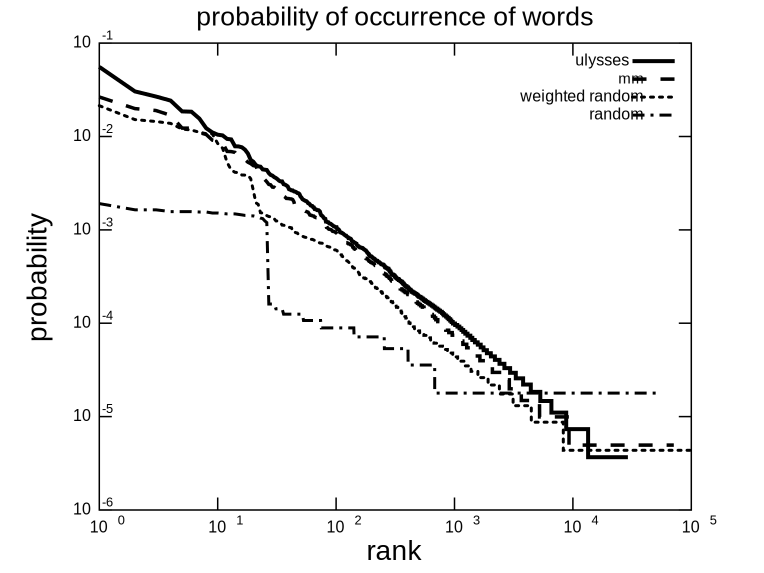
\includegraphics[width=0.8\textwidth]{images/ulysses_compared_words_probabilities.pdf}  
\caption{The rank-frequency distribution of (pseudo-)words in James Joyce's \textit{Ulysses} and random texts using the phones/diphones probabilities. The random curve presents the frequency of occurrence of pseudowords derived by text created by a white process and having the same length as \textit{Ulysses}. The weighted random curve is created by randomly choosing symbols with the same probabilities as the phones in \textit{Ulysses}. The \textit{mm} curve presents the result of a random text derived by a Markov Model where the transition between phones has the same probabilities of the transitions found in \textit{Ulysses}.}
\label{fig:ulysses_compared_words_probabilities}  
\end{figure}  
 
 
Zipf also presents the comparison curve of R. C. Eldridge data, which consists of 
43,989 running words, with 6,002 different words, of combined samples from American
newspapers. The concordance on the curves ``clearly show that the selection and usage
of words is a matter of fundamental regularity of some sort of an underlying governing
principle that is not inconsistent with our theoretical expectations of a vocabulary
balance as a result of the Forces of Unification and Diversification'' \cite{zipf1949}.


The Zipf curves, as presented in Figure \ref{fig:ulysses_compared_words_probabilities}, 
must inherently be a monotonically decreasing curves, since the data is ordered and ranked
according to the frequency of occurrence. \cite{li1992} points that 
``Zipf's law is not a deep law in natural language as
one might first have thought. It is very much related to the particular representation one
chooses, i.e., rank as the independent variable''. 
If Zipf's law arises at randomly generated texts with no linguistic structure, we might conclude
that the law may be a statistical artifact rather than a meaningful linguistic property.

Random generated sequences of letters results in the formation of letter chunks. Those letter chunks
might be sorted according to their frequency of occurrence and, by doing that, chunks of the same
length will present approximately the same frequency, what will create a stair case pattern as presented 
by \citet{li1992}. The decay follows approximately a Zipf's law slope
$(\sim 1/r)$, a power law with exponent $1$ (one). 
The results presented in Figure \ref{fig:ulysses_compared_words_probabilities} shows that
white random text follows clearly a different pattern compared to the natural text,
but as the random generator process assumes certain characteristics, it might have a pattern
closer to the one found in natural texts.

The simple model considered by \citet{li1992} is due to \cite{miller1957,mandelbrot1965}
and it is known as \textit{random typing} or \textit{intermittent silence} model.
It is simply a random generator of characters, where a certain symbol is designed as 
a word-delimiting character. As seen here, the words formed by this approach
show a Zipffian-like frequency behavior, but the number of different words of a certain
length is exponential in length, what diverges from what is observed in a natural language,
since it is in fact not even monotonic.
The \textit{intermittent silence} model might not be used to draw a conclusion that
the Zipf's law is linguistically shallow \citep{mandelbrot1982}, since that model is ``shallow'' itself.


Considering that the probability of occurrence of phones in a random generated text is not uniform,
we experience different results that distance from the white random case and get closer to the natural text.
Figure \ref{fig:ulysses_compared_words_probabilities} presents three different randomly generated texts:
1) equal probability phones, white noise (depicted by dashed-point line); 2) weighted probabilities, using 
the same probabilities of the phones encountered in \textit{Ulysses} (small dashed line); 3) text generated
by a Markov Chain using the states' transitions probabilities equal to the probabilities in \textit{Ulysses} 
(big dashed line).

In a natural language not all combinations of speech structures are possible, and they don't happen
with the same probability. We might observe this when comparing the number of existing words for a given
length. When a random generation process is used, the number of different words (types) will be greater  
then the number of words in a natural language, and that will be valid for every word length.
What we observe is that a natural language presents a higher probability of occurrence for small
words. In our compared example, the highest probability occurs on words of length $4$ and $3$.
This behavior is quite different from the random patter, as we might observe in Figure
\ref{fig:ulysses_compared_word_length_probabilities}.


\begin{figure}[h]
\centering  
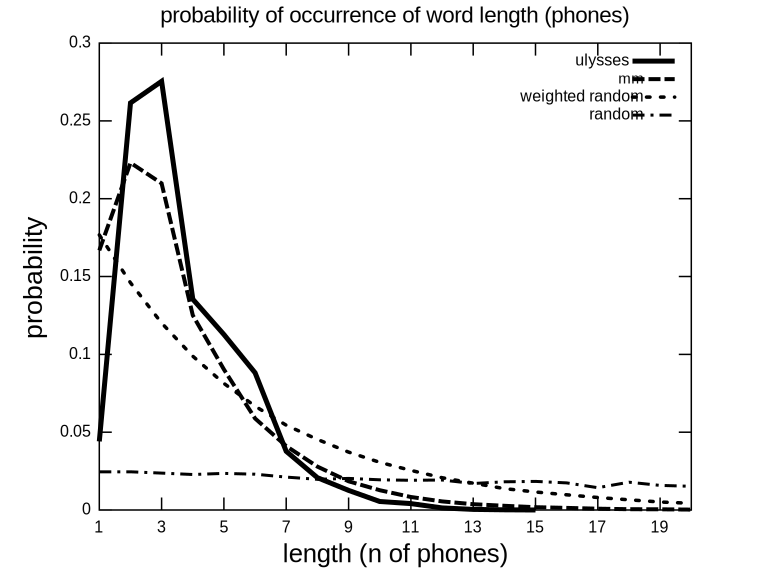
\includegraphics[width=0.8\textwidth]{images/ulysses_compared_word_length_probabilities.pdf}  
\caption{Compared plot of the frequency of occurrence of (pseudo-)words length in \textit{Ulysses} and random texts as described in the text.}
\label{fig:ulysses_compared_word_length_probabilities}  
\end{figure} 

It is important to note that when we consider the random generated texts, we are generating a
string of symbols that we are regarding as phones, and for that reason we consider a set with
the same size of the set of phones. This assumption is made because we are assuming that phones
are our unity of analysis. When we are dealing with natural text, we are using a phonetic
transcription dictionary, as previously stated.

The examples of random generated text in Figure \ref{fig:ulysses_compared_word_length_probabilities}
show that when we consider a weighted probability of occurrence for the randomly generated symbols,
we create the effect of making the shorted pseudo-words more probable, but what we observe in a
natural language is different, we don't see a monotonically decreasing probability, but rather
a peak on words of length $4$. This effect is slightly achieved when we consider a Markov Model with
transitions probabilities equals to the probabilities found in the natural text.
To explain the behavior observed in Figure \ref{fig:ulysses_compared_word_length_probabilities}, we 
might consider the role of three forces: 1) a human cognition ability that makes us assign
shorted codes to more frequent signs, this effect causes a tendency in the probability to 
monotonically decay as the length of words increases; 2) the number of possible symbols chunks that
might be created, regarding that the symbols probabilities are not uniform, this will also 
creates a monotonically decreasing probability patter; 3) there are restrictions imposed on
certain combinations of phones, provoking a greater effect on short words, due to the smaller
amount of possible combinations of symbols. We could also hypothesize that there are restrictions
on the sequence of phones that overcome the immediate vicinity of that phone, and this effect 
would be stronger on phones that are closer, and weaker on phones that are far apart, 
also causesing the smaller probabilities on very
short chunks, where this restriction poses a stronger force, and being overcome on longer ones.







\subsection{The Analysis of Smaller Units}
\label{sec:smaller_units}
In the previous analysis we focused on words as our speech units.
Word is considered the smallest free form that can be uttered or written and carries a meaning.
This is the concept introduced by \citet{bloomfield1926}, but it is doubtful, since some words are not
minimal free forms, like \textit{the} and \textit{of}, which carry no meaning by themselves.
The status of words in a language is still a topic over debate and with not clear answers.
``Words are units at the boundary between morphology and syntax serving important functions as carriers of both semantic and syntactic information and as such are subject to typological variation. In some languages words seem to be more clearly delimited and more stable than in others. The structural make-up of words depends on typological characteristics of languages'' \citep{coulmas}.


The main concern in Phonology is the study of language, as a means of spoken communication, that is built as a system
created by sounds and structures. Under the phonological assumption, 
the concept of sound is not restricted at the physical level of speech
realization, but also extends to symbolic level, where \textit{sounds} are cognitive abstractions
that provide the means for the representation of a language.

The Swiss linguist Ferdinand de Saussure is responsible for
shifting the way linguistic was done and established a break point with his posthumous
publication \textit{Course in General Linguistics} in 1916.
Although many years have passed, the central concept of relating sound to meaning in a structured way 
has remained the same. In Saussure's model, the linguistic sign has three aspects: 
physical (sound waves), physiological (audition and phonation) and psychological (sounds as abstract units,
which he calls `sound images').

The concept of \textit{sound images} was represented by the phoneme, regarded as a linguistic distinctive unity
which groups different sounds into single and not superposed categories.
Each language has its own phoneme inventory, which is created by what are the possible distinctions made between 
speech sounds in each language. For example, English makes no distinction between aspirated and unaspirated sounds,
but in Hindi such distinction exists \citep{ladefoged1996}.
Implicit in the idea of phoneme is that language may be segmented into a sequence of
consecutive symbols in time. %Beno\^it Mandelbrot 
\citet{mandelbrot} showed it is an important requirement
in order to make speech a comprehensible communication process in most situations,
especially under heavy corruption. This discrete aspect of language guarantees the discreteness at all other levels
of the language analysis, what is the basis of our linguistic knowledge.


As pointed out by \citet{capek1983}: ``Saussure did not discover -- or invent -- the phoneme.
He was one of a number of scholars working on comparable ideas. His statements are
important not so much for the accuracy with which they report facts or for their strength
and consistency as for the explanatory power of the inferential network they set up. Suffice
it to say that after Saussure the clumsy terminology used by scholars who preceded him --
that of speech sounds (Sprachlaute) -- came to be replaced by the much more intuitively
satisfactory concept of the phoneme.''


The term \textit{phoneme} was proposed by the linguist Dufriche-Desgenettes
as a substitute for the German \textit{Sprachlaut} (\textit{speech sound}) in the early 1870s \citep{dresher2011}.
It had, by that time, the meaning of what we now call \textit{speech sound} or \textit{phone}.
The concept of \textit{phoneme} changed with Saussure, who used it ``to refer to a hypothesized sound in a 
proto-language together with its reflexes in the daughter languages'' and further the meaning was 
recast by Kruszewski, bringing the synchronic notion, that we have today, of a set of alternating elements 
that were interpreted by Baudouin as an invariant psychophonetic element that may be realized in different forms
and as proposed by Jones, a family of sounds that, for practical purposes, are
accounted as the same \citep{dresher2011}. Today the phoneme no longer holds a central place
in phonology theory, but it has not disappeared from phonological theory nor its demise has come.
Although many evidences have risen questioning the phoneme status \citep{port2007,port2005,port2006}, 
its definition and properties, it seems more as a symptom of a theory of phonology that is not 
completely defined yet.


``The point of concern at present, however, is not to
devise a system of symbols whereby the sequence of sub-gestures constituting a speech-sound 
can be noted, but rather to remark that speech-sounds and phonemes may be
viewed as constellations, or configurations, of articulatory sub-gestures, arranged partly
or completely in sequential order, some sequences running concurrently with others (e.g.
the occlusion is concurrent with the voicing of \textit{d}). Although there is not a single speech-sound, 
or variant form, of a phoneme in any language which cannot be conceived of as a
constellation or configuration of the type envisaged above, yet a complete and accurate
description of even a single speech-sound in terms of sequences is practically impossible.
However, by conceiving phonemes as constellations of this order, we have found a very
useful method of comparing a number of specific phoneme pairs which have essential
sequences in common''\citep{zipf1949}.


The units of language (phonemes, syllables and words) are well represented in a writing system,
for the process of writing requires the dissection of the
speech stream into its constituents distinguishable parts. The process of dissection happens in
different levels, so that the assemblage of its parts creates meaning on the speaker discourse.
``Every writing system maps onto a linguistic system, it embodies and visibly exhibits the 
dissection of units of language and thus linguistic analysis''\citep{coulmas}.
It is reasonable then to investigate the patterns and structures of a language through its
written counterpart.


In order to perform such analysis, we used the text \textit{Ulysses} from
Joyce, and created a transcription from written text to phones sequence. 
The Carnegie Mellon University (CMU) 
Pronouncing Dictionary \citep{cmu2008} was used to get the phonetic transcription of each word in our database,
according to the General American (GA) English, which is
the major accent of American English. 
In the CMU Pronouncing Dictionary, words are coded by the phonetic transcription code \textit{Arpabet},
where each code is a distinct sequence of ASCII characters.
GNU tools, Python and Octave scripts were used to process and analyze the data.


\subsection{Phones, Diphones and Triphones}
\label{sec:phones}
In this section we present the results observed as we draw a Zipf plot of the phones, diphones and
triphones, comparing the natural text with the random generated texts, as previously described.
Figure \ref{fig:ulysses_compared_phones_probabilities} presents the compared probability of occurrence
of phones. As all random texts were generated using the phone probabilities or
transition probabilities from \textit{Ulysses}, they presented the same behavior, only the
white random process shows a different result, since all phones are equiprobable.
There are 39 phones, and from a visual inspection of Figure \ref{fig:ulysses_compared_phones_probabilities}
we might conclude that the Zipf's law does not holds for this very small set of symbols,
%we could conclude that the first 28 phones follow a Zipf relation different from the other 11 phones.
%We observe that it does not follow a Zipfian
%distribution, 
but instead a logarithmic relation exist, as also pointed by \cite{kanter1995}.
As we analyze higher order structures, we shall notice that it will progressively approach 
a Zipf's relation as we go from phones to diphones, then from diphones to triphones, until
we reach the words' level, which clearly presents a Zipf's law.
%There is a clear change in behavior that is not found when we analyze higher level structures,
%such as diphones, triphones, and words.


\begin{figure}
\centering
\begin{tabular}{cc}
  \subfloat[Comparison of phone frequency of occurrence. All three curves present the same pattern.]{\label{fig:ulysses_compared_phones_probabilities}\includegraphics[width=0.45\textwidth]{images/ulysses_compared_phones_probabilities.pdf}} &
  \subfloat[Comparison of diphone frequencies of occurrence. The behaviour of diphone frequencies generated by the white and weighted random text diverges from the others.]{\label{fig:ulysses_compared_diphones_probabilities}\includegraphics[width=0.45\textwidth]{images/ulysses_compared_diphones_probabilities.pdf}} \\
  \subfloat[Comparison of triphone frequencies of occurrence. The behaviour of triphone frequencies generated by the Markov Model does not follow closely the pattern presented in \textit{Ulysses} as was still observed with diphones.]{\label{fig:ulysses_compared_triphones_probabilities}\includegraphics[width=0.45\textwidth]{images/ulysses_compared_triphones_probabilities.pdf}} &
  \subfloat[Frequency of occurrence of syllables in \textit{Ulysses}. The syllabification was done computationally using online dictionaries.]{\label{fig:ulysses_syllables_probabilities}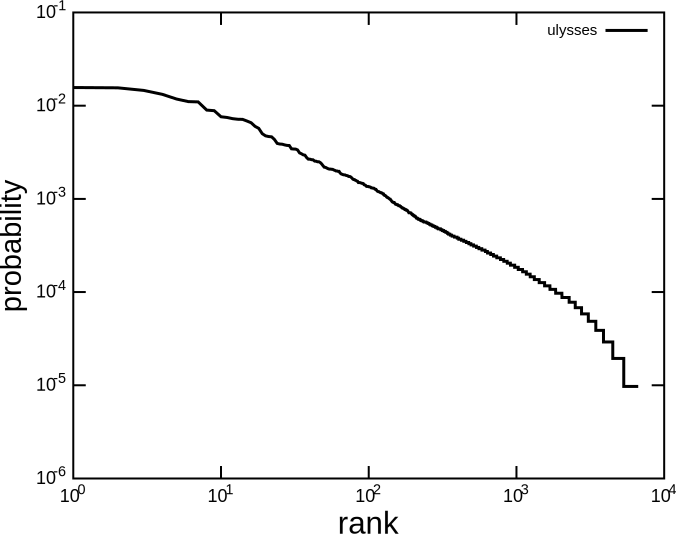
\includegraphics[width=0.45\textwidth]{images/ulysses_syllables_probabilities.pdf}}    
\end{tabular}
\caption{Compared frequency of occurrence plot for phones, diphones and triphones in \textit{Ulysses} and in random texts generated as previously described, a white random source; a weighted random source with phones probabilities equal to the one found in \textit{Ulysses}; and a Markov model with transition probabilities between phones as the probabilities in \textit{Ulysses}.}
\label{fig:ulysses_compared_nphones_probabilities}
\end{figure}


It is interesting to observe how phones occur in a language and the way they relate with one another
creating higher order structures under different constraints. The acquisition of a language is 
based on tracking those multiple regularities in the input stimuli. Only if we analyze long data
it will be possible to observe emergent regularities, and the more complex the regularities under
observation are, the more data will be needed to stablish a distinction among those regular patterns.
Those regularities are known as grammatical structure of a language, and since early ages, 
infants can perceive the difference of grammatical and ungrammatical sentences \citep{Saffran2003}.


The plot in Figure \ref{fig:ulysses_compared_diphones_probabilities} 
shows the probability of occurrence of diphones found in the same texts described before.
The white random process still preserves the equiprobability on the occurrence of diphones.
The Markov Model still follows very closely our reference text, and our zero order model 
does not present the same characteristic as the reference. 
When we take into consideration transition probabilities as our source model, 
we observe that the formation of some diphones is facilitated, while the formation of others 
is hardened. The behavior of phones clearly doesn't agree with a power law relation, but
not, observing the behavior of diphones we start to see a Zipf's law being created, as a result
of the increase on the length of our symbol set.
%The behavior of phones could be thought as two different Zipf laws, now the behavior of
%diphones might be interpreted as two Zipf laws with a smooth transition between them. 

As we move forward from phones, diphones and triphones to larger chunks, 
what we may observe is that the behavior gets closer to
the Zipf law observed when we analyzed words as our structural blocks. 
%It is still not 
%possible to state a single law to describe the observed data, but it grows near the word behavior
%in a Zipf plot. 
Observing the compared plot stated in Figure \ref{fig:ulysses_compared_triphones_probabilities}
we might observe that only the Markov model follows closely the natural behavior of triphones.
The frequency of occurrence, or predictability, of a speech unit is believed to be related to
its complexity when regarding acoustic realization \citep{jurafsky2001}, and the complexity is 
further associated with the duration of the given structure. Using annotated speech corpora,
\citet{jurafsky2001} concluded that when regarding the frequency of occurrence of n-phones as a function of its
duration, the relation is an inverted U-shape curve, so that short n-phones have smaller 
probability of occurring than middle-length n-phones and longer n-phones also have smaller 
probability. Comparing the frequency of occurrence of words for a given length we 
observed different results as we regarded phones or syllables as our building units for the words.
As previously shown in Figure \ref{fig:ulysses_compared_word_length_probabilities},
short words have smaller probabilities than middle length words, and the peak occurred in 3 phone
long words. When the length of a word is regarded as the number of syllables, then we
observed a monotonically decaying curve of probability of occurrence of words versus 
word length. Although there is not a clear straight relation between the number of syllables in a word
and its duration, from our observations in Section \ref{sec:words_length}, 
it seems reasonable to infer that the duration is proportional,
and that would lead again to the conclusion that, on higher order analysis, the 
behavior observed in the frequency of occurrence of words is different from its constituent parts.
The U-shape curve is reshaped into a straight line as syllables or phones are combined to build up
words.

It seems fascinating that languages and other natural phenomena, all of them a result of 
different complex systems, share a certain property which is described by a single simple law.
The same patterns are also observed when analyzing words and n-phones in different languages.
\cite{miller1965} proposes two different approaches to explain the ubiquitous observation of
Zipf's law: ``Faced with this massive statistical regularity, you have two alternatives.
Either you can assume that it reflects some universal property of human
mind, or you can assume that it reflects some necessary consequence of
the laws of probabilities. Zipf chose the synthetic hypothesis and searched
for a principle of least effort that would explain the apparent equilibrium
between uniformity and diversity in our use of words. Most others who
were subsequently attracted to the problems chose the analytic hypothesis
and searched for a probabilistic explanation. Now, thirty years later, it
seems clear that the others were right. Zipf's curves are merely one way
to express a necessary consequence of regarding a message source as a
stochastic process''.

Larger units of speech are used as recognition units to model the coarticulatory effects,
for example, syllables and triphones. The last one is quite often used in phonemic based
speech recognition, for the context of a given phone is established by its preceding and
following neighbors. 
The more features subsequent phonemes share, more easier will be the articulation of this 
sequence, since the transitions tend to be smother. On the other hand, it is important 
to create contrast between adjacent phonemes, so that one phone is distinguishable
enough from the phone next to it, what will enhance discriminability. This tradeoff
might be perceived on the triphones usage profile. 
Figure \ref{fig:ulysses_triphones_intradistances_mesh} presents the probability of occurrence of
triphones given their intradistances. For each triphone, two distances are calculated: the
distance from the second to the first phone; and the distance from the last to the middle phone.
The distance measure used is the number of distinctive features not shared by two phones under comparison,
as is explained in Chapter \ref{cp:featuretheory}. The number of occurrences of each triphone occurring in 
\textit{Ulysses} was added up 
according to its intradistances and the final probability of occurrence for each intradistance pair 
was calculated. We might observe in Figure \ref{fig:ulysses_triphones_intradistances_mesh}
that the most occurring triphones are those with medium intradistances, which appear as
a peak. That makes evident the tradeoff, previously argued, between articulatory ease and contrast.  
Triphones with small and large intradistances are seldom used, and some intradistance pairs
(26 in the total, which represent 11.5\% of the 225 possibilities) are not used at all.


\begin{figure}[h]
\centering  
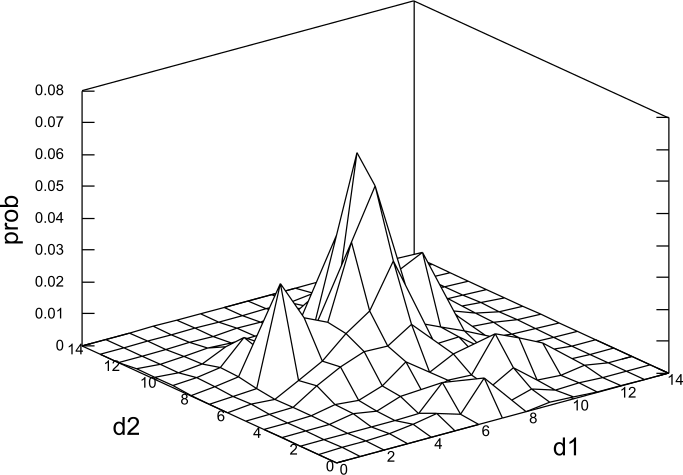
\includegraphics[width=0.8\textwidth]{images/ulysses_triphones_intradistances_mesh.pdf}  
\caption{Given the intradistances in a triphone (the distance from the second to the first phone, $d_1$, and the distance from the third to the second phone, $d_2$), the probability of occurring triphones in \textit{Ulysses} is presented. Triphones privileges medium intradistances, having a peak when the intradistances are around 8. The distance function used the number of non-shared distinctive features.}
\label{fig:ulysses_triphones_intradistances_mesh}  
\end{figure} 


Figure \ref{fig:ulysses_triphones_intradistances_mesh} shows that there is a strong relationship 
between adjacent phones in a triphone structure, where the inter-distance between phones tend to
an average value, and extreme values are not usual. It is natural then to speculate what would be
this kind of relation within words. Figure \ref{fig:ulysses_words_intra_phone_distance_freq_occ_avg_std}
provides an analysis of the inter-phone distances within words. It presents, in a logarithmic scale,
the frequency of occurrence of words for a given relation between the average inter-phone distances and 
the standard deviation of the inter-phone distances. Once again, the distance metric used is the number
of distinctive features not shared by two phones. Among the plotted data, we observe no tendency of increased
occurrence of words for a certain relation between average and standard deviation of inter-phone distances.
The plot of the number of words for a certain relationship of their inter-phone distances present a similar
pattern, and normalizing the frequency of occurrence chart by chart with the number of words, we
conclude that there is no aid making some inter-phone distance relation more probable than others.
What we might observe from our chart and analysis is that there is a relationship between the
average value and the standard deviation value for the inter-phone distances: when the average distance
decreases, the deviation increases as a compensatory effect, for words have to maintain a certain phonemic 
variability within. The correlation coefficients (Pearson product-moment correlation coefficient)
between the mean value and the standard deviation observed in the inter-phone distances within words
is $-0.67$ and p-values for testing the hypothesis of no correlation
(assuming that the true correlation is zero, the p-value is the probability of getting a correlation as large 
as the observed one)
is null.


\begin{figure}[h]
\centering  
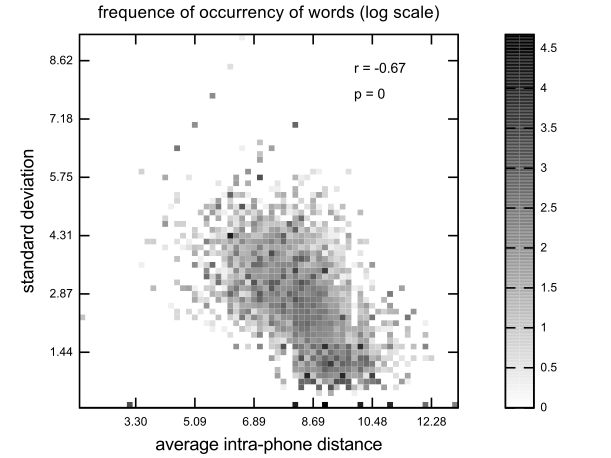
\includegraphics[width=0.8\textwidth]{images/ulysses_words_intra_phone_distance_freq_occ_avg_std.pdf}  
\caption{The words frequency of occurrence  in \textit{Ulysses} is presented in a logarithmic scale as a function
of the average intra-phone distances and the standard deviation of these distances. The relationship
between the number of existing words as a function of average and standard deviation of distances follows
a similar pattern and our analysis doesn't show any effect that frequency has on this pattern. 
What we might observe is the tradeoff between average intra-phone distance and standard deviation, 
as the mean distance value decreases, the deviation increases as a compensatory effect. 
The correlation coefficient observed in this data (with 19,150 samples) is $-0.67$.}
\label{fig:ulysses_words_intra_phone_distance_freq_occ_avg_std}  
\end{figure} 


In order to analyze the variability of triphones that may be formed by a certain phone, 
when regarding the transitions of distinctive features in a triphone, we 
considered the difference of the distinctive feature vectors between the middle phone
(reference) and the first and last phones. As each reference phone occurs in many
triphones combinations, we create a weighted sum of all these difference feature vectors, 
where the weight factor is the probability of occurrence of each triphone. For each
phone we have built two vectors: one from the differences with the previous phone
and the other from the differences with the next phone.
Each of these vectors is represented by a column in the image presented
in Figure \ref{fig:phone_triphone_varialibity_dist_features_sorted2}.
It is presented as shades of gray, when the gray level approaches white,
then there is more variability (the difference is greater) and when it approaches
black, there is less variability (the difference is smaller).
We have ordered the features sorted by the accumulated variability across 
all different triphones for all phones in the set. The cumulative curve is plotted on the right. 
We also ordered the phones
by the variability observed on their triphones. Each pair of columns 
in the image presented in Figure \ref{fig:phone_triphone_varialibity_dist_features_sorted2}
corresponds to one phone that is transcribed in the axis bellow.
The bottom curve in Figure \ref{fig:phone_triphone_varialibity_dist_features_sorted2}
presents the variability for each phone, 
displaying
the differences with the previous phone (left) and the differences with
the next phone (right) in a triphone set.
We might conclude that the features presented are sorted by their distinctiveness 
capabilities, that is: \textit{syllabic}, \textit{consonantal}, \textit{sonorant}, \textit{coronal}, 
\textit{back}, \textit{front}, \textit{continuant acoustic}, \textit{voice}, \textit{high}, 
\textit{strident}, \textit{labial}, \textit{approximant}, \textit{nasal}, \textit{distributed},
\textit{dorsal}, \textit{tense}, \textit{lateral}, \textit{labiodental}, \textit{delayed release}, 
\textit{spread glottis}, \textit{trill}, \textit{tap} and \textit{constricted glottis}.


From the bottom plot in Figure \ref{fig:phone_triphone_varialibity_dist_features_sorted2}
we might conclude that the variability between the first and the middle phones in a triphone
is always greater than the variability between the middle and the last phones.
Since every two side-by-side points corresponds to one certain phone, and they are always arranged 
in the order mentioned before (1st-2nd phones, 2nd-3rd phones), 
we observe that within each pair the curve presents a negative slope,
and for that reason we might conclude that the first phone pair (1st-2nd phones) has a greater distinctive
feature variability in every triphone.
As we analyze larger chunks, we verify that this decreasing behavior on the average distance
between phones does not hold anymore.

\begin{sidewaysfigure}
%\vspace{12cm}
\centering  
\includegraphics[width=0.8\textwidth]{images/phone_triphone_varialibity_dist_features_sorted2.pdf}  
\caption{This picture presents the variability of distinctive features within triphones for a given
middle phone taken as reference. The distinctive features are sorted by their total variability 
(across all triphones) and the reference phones are sorted by the total variability across of its 
features within its set of triphones. The shades of gray represent the variability of a given 
feature within a give triphone. The white color correspond to the greatest variability and the
black color to the smallest variability.}
\label{fig:phone_triphone_varialibity_dist_features_sorted2}  
\end{sidewaysfigure}




Preliminary studies show the existence of consistent frequency distribution patterns in other languages.
These regularities are believed to be a result of language as a stochastic process and a product
of usage and self-organization. If the underlying principle of organization of languages is the same,
we are supposed to observe similar patterns when analyzing language statistics.







\section{Length of Words}
\label{sec:words_length}
The study of language, under a phonological point of view, presupposes
the discretization of the speech stream into unities, which are subject to rules.
Phonological theories are based on the discretization of speech into segments
that assembles themselves according to certain rules to create higher order
structures. 
Words are assumed as discrete entities built over other discrete
units, such as syllables, morphemes and phonemes.

Words are argued to be unities of mental representation,
although the very concept of word is still, in some aspects, unclear.
\cite{bloomfield1926} introduced the concept of words as the 
smallest free form that may be uttered in isolation carrying a semantic 
or pragmatic content of its own, but it is doubtful since some words are not minimal free forms.
It is fair to question whether or not
the definite and indefinite articles, \textit{the} and \textit{a}, are themselves words at all.
Do they carry a meaning of their own? 
There are also those meanings that require two strings of letters to express themselves, like: 
\textit{stock market}, \textit{apple tree}, \textit{carbon dioxide}, \textit{dental floss}, among others. 
What about \textit{compound words}? Is every \textit{compound word}
a word? Or a composition of words as the name suggest? 
There are many examples of \textit{compound words}: \textit{newspaper}, \textit{thumbnail},
\textit{copperhead}, \textit{eyelid}, \textit{bedroom}, among many others;
and there is also a tendency of some to become a \textit{compound word}, for example:
\textit{hot dog} it also written as \textit{hotdog}.
The compound word \textit{blackboard}
is just a combination of the words \textit{black} and \textit{board} that happens to designate
an object that is not black at all. What amount the uncountable examples that an analytical language
as German is capable of creating? The word for \textit{blackboard} in German is \textit{Tafel}, but
it could also be \textit{Wandtafel}, which is just a compound made of \textit{Tafel} and \textit{Wand}
(Wall). The German word \textit{Streichholzschachtel} (matchbook), is made of
\textit{streichen} (scratch), \textit{Holz} (wood), \textit{Schachtel} (box), while the English
word \textit{matchbox} is also a compound but made of \textit{match} (not the Football one) and
\textit{box}. The way they are built is quite different, but make reference to the same object.
That is something that tells about the way languages are structured and used, and it might be
possible that the structures are a bit different in every language. 

\cite{olson1994} stresses the point
that the concept of the word as distinct unit is a by-product of literacy acquisition.
The analysis of antique texts revels that texts were commonly redacted in \textit{scriptura continua},
that means `without word boundaries' \citep{saenger}. The continuous string of characters 
was just a rightful representation of what speech utterances truly are.
According to \citep{saenger1997}, the lack of boundaries between words causes 
two drawbacks in the reading process: it slows down reading and encourages vocal activity.
If the writing is dense and devoid of `distinguishing signs', the decoding process
is considerable longer and rely on vocalization. Silent and rapid reading is an achievement 
of our civilization which resulted from the development of a system of graphic signs in which
the blank space is of prime importance. ``In the sixth century, all manuscripts were still copied
in \textit{scriptura continua}, and it was not until between the sixth and eighth centuries that the
separation of words was progressively introduced into all Latin manuscripts'' \citep{pombo2002}. 
Literacy is indeed an influential ability in our languages skills. As pointed by \cite{hagege1986}
``writing is a linguistic analysis in various degrees of awareness''.

There are many interactions between speech and writing. Lev S. Vygotsky was a
psychologists who took an active interest in the cognitive consequences of writing,
studying how speech affected writing and vice versa. 
``Writing requires deliberate analytic action on the part of the speaker\footnote{Originally Lev S. Vygotsky was talking about \textit{child}, but we made the substitution to comprise a wider context which
we believe is still valid.}.
In speaking, he is hardly conscious of the sounds he produces and quite unconscious of
the mental operations he performs. In writing, he must take cognizance of the
sound structure of each word, dissect it, and reproduce it in alphabetic symbols,
which he must have studied and memorized before''\citep{vygotsky}.
The relationship between writing systems and spoken language is also a theme covered
by \cite{coulmas}. According to him, ``the introduction of writing implies a 
cognitive reorientation and a restructuring of symbolic behaviour. Names of objects
are conceptually dissociated from their denotata, as signs of physical objects are
reinterpreted as signs of linguistic objects, names. In a second step, signs of names
are recognized as potentially meaningless signs of bits of sound, which are then
broken down into smaller components'' \citep{coulmas}.

Considering words as unities of mental processing, it is important to investigate
the aspects involving this hypothesis. \cite{miller1956} suggested that the short-term memory
storage capacity is constant in terms of the number of chunks. If we could consider words as
chunks, then the short-term memory capacity should be the same regarding the size or duration
of words.
\cite{Baddeley1975} explores the relations between the memory span\footnote{Memory span is a common
measure for short-term memory, where it is related to the length of a list of discrete items a person 
is capable of memorize and repeat back in order after presentation with an accuracy equals of superior
to 50\% of all trials. It appears to measure one's capacity to successfully distribute his attention
and organize the incoming stimuli as a working unit.
} and length of words.
They observed that memory span is inversely proportional to word's length. Word's duration
was recognized as an important aspect, since it was recognized that words of short temporal duration were 
better recalled than words of long duration, even when the number of syllables and phonemes 
are held constant. 
The results achieved by \cite{Baddeley1975} have some implications on \cite{miller1956}'s 
suggestions, ``that memory span is limited in terms of number of chunks of information, rather that their
duration. It suggests a limit to the generality of the phenomenon which Miller discusses,
but does not, of course, completely negate it. The question remains as to how much
of the data subsumed under Miller's original generalization can be accounted for in terms
of temporal rather than structural limitations''\citep{Baddeley1975}.

\cite{neath1995} points that ``current explanations of the word-length effect
rely on a time-based decay process within the articulatory loop structure in working memory'',
what does not completely explain one of the observations made by \citep{Baddeley1975}: ``when
articulation is suppressed by requiring the subject to articulate an irrelevant sound, the
word length effect disappears with visual presentation, but remains when presentation is
auditory''. \cite{neath1995} concludes that ``word-length effects do not offer sufficient
justification for including time-based decay components in theories of memory''. He proposes
then a feature model \citep{nairne1988, nairne1990} where the interferences handles 
the explanation of the observed data.
It was designed to account for the major effects observed in immediate memory settings,
what includes the recency effect, the effects of articulatory suppression, temporal grouping, and
phonological similarity, among others. 

In order to better understand the role played by these aspects into the way a language is
structured, organized and used, we propose here a statistical analysis using a corpus. 
It would be time-spending and would require a great amount of work to collect a speech corpus
and make use of it. Instead, we propose the usage of a text corpus, pronunciation dictionary
and speech samples provided by online dictionaries.
The analysis here will concern only the statistical aspects of written and spoken words length,
what is important as length is regarded as an aspect of mental representation, 
among other features \citep{port2007}.

Mendenhall realized that the study of word length, specifically, the analysis of the distribution
of words of different lengths was important to establish comparisons of styles. \cite{mendenhall1887}
investigated the differences in the literary 
styles of Dickens and Thackeray insofar as word-length distribution was concerned. The same approach
was afterwards used \citep{mendenhall1901} to analyze the authorship of Shakespeare's plays\footnote{
The Shakespeare authorship question was first posed in the middle of the 19th century,
when the flattery of Shakespeare as the greatest writer of all time had become widespread.
More than 70 authorship candidates have been proposed, including Francis Bacon.}.
In every Shakespeare's play the count of words of length four was always greater than the count of
words of length three. Comparing with Bacon, the count of words of length three was greater than four, and
Bacon also present a distinctly higher proportion of longer words than Shakespeare.

Mandelbrot \citep{mandelbrot} supposes that words are built of a sequence of elementary unities and the process of 
assembling those unities into a speech stream is an elementary additive process. The cost
assigned to this process is a compound of the number of building blocks used and their characteristics.
The probability of occurrence 
of each word is assigned so that, on a long sequence, the average word-information-content
is maximized, being also subject to the additive costs of building each unity and the sum of
all the relative frequency of occurrence (probabilities) of each word must be one. Making the choice
that leads to such maximization is performing an entropy\footnote{As defined by Shannon, 
the entropy is an additive measure of the amount of available choice 
in the process of selecting one from the allowable messages among many in each unit of
the information transmission process. Entropy is used as a measure of the amount of information
carried by a random variable.} maximization.
The sender should maximize the transmission rate of information and concomitantly minimize
the cost of transmission. This cost was expressed as a function of the length required in the transmission
process, making short words a preferred choice. Mandelbrot demonstrated that a word-by-word encoding
of a message will lead to the observed rank-frequency relation in natural languages.

Using our database we are able to estimate the number of words for a given length and
also how frequently words of this length are used. The Figure \ref{fig:wordsNumVsLength} presents
these results. When the length of a word increases, the number of possible combinations of
building unities increases factorially, but what we observe is an increase as short length words
become longer and a great decrease after a turning point. The usage of shorter words, as expected,
is greater, and the small drop observed for small words is just a consequence of the fewer 
number of possible combination leading to the existing words with short length words. 
When the frequency of occurrence curve is normalized
by the the number of existing words, we get a monotonically decreasing line, as expected 
(Figure \ref{fig:wordslengthfreqnorm_en} and \ref{fig:wordsphoneslengthfreqnorm_en}). 
This is corroborated when we take the average word length across
words rank, as pictured in Figure \ref{fig:averagewordslength_en} and \ref{fig:averagewordsphoneslength_en}
the words with smaller rank are on average also smaller, either in the number of letters, phones
or syllables.

Figures \ref{fig:wordsFreqOccurrenceRange} and \ref{fig:phonesFreqOccurrenceRange}
present how the usage of words and phones is different when analyzing words of different
length (number of letters, number of phones or number of syllables).
It is possible to verify that in the extreme cases, when we analyze words of short length or 
long length, the pattern observed in the rank vs. frequency plot is quite different from the
middle length words. The short and long words experience steeper decay regarding the occurrence
of words or phones.


The relationship between the number of Phones and the number of Letters and 
the number of Phones and the number Syllables may be observed in 
Figure \ref{fig:wordsLettersPhonesSyllablesNumberOfWordsLog}.
Phones and Letters have a straight line relationship, and the majority of the words
have between 3 and 9 letters and 3 and 10 phones.
The relationship between number of phones and syllables is a little more dispersed,
and we may observe that the majority of words have between 1 and 3 syllables, corresponding
to the range of 3 to 9 phones. 

When considering the frequency of usage of words with a certain number of syllables and phones,
or phones and letters, we observe a more diffuse relation that still resembles the relations
regarding the number of words. This might be observed in 
Figure \ref{fig:wordsLettersPhonesSyllablesFreqOccurrenceLog}.

Another way to regard words length is to measure its duration when uttered.
Although each speaker will utter the same word with a different duration at each
trial, on the average, and under normal conditions, we expect to observe the same
duration, what might not differ much from one speaker to another, unless 
one suffer from some sort of aphasia, compromising the speaker elocution capabilities,
or he is under a certain situation in which he is required to speak on a much slower or 
faster rate. The data then here analyzed consists of utterance duration of words
collected from online dictionaries. The samples where collected from each dictionary and
its duration were afterwards normalized within each group. Unfortunately each dictionary has
samples from different speakers and there is no control under the speech rate used.
Although the data don't present
a strong correlation it is not so weak and we might observe, in Figure \ref{fig:dicutterduration},
that the relation between number of syllable and duration of the uttered word is
more diffuse then the previous relations presented before, but still there is a 
straight line tendency.


\begin{sidewaysfigure}
  \centering
  \subfloat[number of letters.]{\label{fig:wordsNumVsLetterLength}\includegraphics[width=0.3\textwidth]{images/wordsNumVsLetterLength.pdf}}                
  \subfloat[number of phones]{\label{fig:wordsNumVsPhoneLength}\includegraphics[width=0.3\textwidth]{images/wordsNumVsPhoneLength.pdf}}    
  \subfloat[number of syllables]{\label{fig:wordsNumVsSyllableLength}\includegraphics[width=0.3\textwidth]{images/wordsNumVsSyllableLength.pdf}}    
  \caption{Number of words in the English with a certain length, measured as the number of letters, phones or syllables.}
  \label{fig:wordsNumVsLength}

  \centering
  \subfloat[number of letters.]{\label{fig:wordsFreqOccurrenceVsLetterLength}\includegraphics[width=0.3\textwidth]{images/wordsFreqOccurrenceVsLetterLength.pdf}}                
  \subfloat[number of phones]{\label{fig:wordsFreqOccurrenceVsPhonesLength}\includegraphics[width=0.3\textwidth]{images/wordsFreqOccurrenceVsPhonesLength.pdf}}    
  \subfloat[number of syllables]{\label{fig:wordsFreqOccurrenceVsSyllableLength}\includegraphics[width=0.3\textwidth]{images/wordsFreqOccurrenceVsSyllableLength.pdf}}    
  \caption{Frequency of occurrence of words in the English with a certain length, measured as the number of letters, phones or syllables.}
  \label{fig:wordsFreqVsLength}
\end{sidewaysfigure}


\begin{sidewaysfigure}
  \centering
  \subfloat[number of letters.]{\label{fig:wordsFreqOccurrence01-09Letters}\includegraphics[width=0.3\textwidth]{images/wordsFreqOccurrence01-09Letters.png}}                
  \subfloat[number of phones]{\label{fig:wordsFreqOccurrence01-09Phones}\includegraphics[width=0.3\textwidth]{images/wordsFreqOccurrence01-09Phones.png}}    
  \subfloat[number of syllables]{\label{fig:wordsFreqOccurrence01-07Syllables2}\includegraphics[width=0.3\textwidth]{images/wordsFreqOccurrence01-07Syllables2.png}}    
  \caption{Frequency of occurrence of words in English with length in a certain range, measured as the number of letters(\ref{fig:wordsFreqOccurrence01-09Letters}), phones(\ref{fig:wordsFreqOccurrence01-09Phones}) or syllables(\ref{fig:wordsFreqOccurrence01-07Syllables2}).}
  \label{fig:wordsFreqOccurrenceRange}


  \centering
  \subfloat[number of letters.]{\label{fig:phonesFreqOccurrence01-09Letters}\includegraphics[width=0.3\textwidth]{images/phonesFreqOccurrence01-09Letters.png}}                
  \subfloat[number of phones]{\label{fig:phonesFreqOccurrence01-09Phones}\includegraphics[width=0.3\textwidth]{images/phonesFreqOccurrence01-09Phones.png}}    
  \subfloat[number of syllables]{\label{fig:phonesFreqOccurrence01-07Syllables}\includegraphics[width=0.3\textwidth]{images/phonesFreqOccurrence01-07Syllables.png}}    
  \caption{Frequency of occurrence of phones in English within words with length in a certain range, measured as the number of letters(\ref{fig:phonesFreqOccurrence01-09Letters}), phones(\ref{fig:phonesFreqOccurrence01-09Phones}) or syllables(\ref{fig:phonesFreqOccurrence01-07Syllables}).}
  \label{fig:phonesFreqOccurrenceRange}
  
\end{sidewaysfigure}


\begin{sidewaysfigure}
  \centering
  \subfloat[Letters and Phones.]{\label{fig:wordsLettersPhonesNumberOfWordsLog}\includegraphics[width=0.3\textwidth]{images/wordsLettersPhonesNumberOfWordsLog.png}}                
  \subfloat[Phones and Syllables.]{\label{fig:wordsPhonesSyllablesNumberOfWordsLog}\includegraphics[width=0.3\textwidth]{images/wordsPhonesSyllablesNumberOfWordsLog.png}}      
  \caption{Number of English words with a certain number of letters, phones and syllables.}
  \label{fig:wordsLettersPhonesSyllablesNumberOfWordsLog}

  \centering
  \subfloat[Letters and Phones.]{\label{fig:wordsLettersPhonesFreqOccurrenceLog}\includegraphics[width=0.3\textwidth]{images/wordsLettersPhonesFreqOccurrenceLog.png}}                
  \subfloat[Phones and Syllables.]{\label{fig:wordsPhonesSyllablesFreqOccurrenceLog}\includegraphics[width=0.3\textwidth]{images/wordsPhonesSyllablesFreqOccurrenceLog.png}}      
  \caption{Frequency of occurrence of words in English with a certain number of letters, phones and syllables.}
  \label{fig:wordsLettersPhonesSyllablesFreqOccurrenceLog}

\end{sidewaysfigure}



\begin{sidewaysfigure}
  \centering
  \subfloat[Scatter plot of words utterance duration from four different dictionaries.]{\label{fig:corrWordsDurationDics}\includegraphics[width=0.3\textwidth]{images/corrWordsDurationDics.png}}                
  \subfloat[Histogram of words mean (across the four different dictionaries) utterance duration.]{\label{fig:histWordsMeanDuration}\includegraphics[width=0.3\textwidth]{images/histWordsMeanDuration.pdf}}
  \subfloat[Number of words with a certain number of syllables and a certain duration.]{\label{fig:numWordsSyllableVsMeanDuration_log}\includegraphics[width=0.3\textwidth]{images/numWordsSyllableVsMeanDuration_log.pdf}} 
  \caption{The data here presented uses the utterances duration of speech samples from the four following on-line dictionaries: Cambridge, Dictionary.com, The free dictionary and Macmillan. The durations were first normalized within each set from each dictionary. Only the words found in all the four dictionaries were used.}
  \label{fig:dicutterduration}
\end{sidewaysfigure}






%
%
%
\section{Menzerath's law}

\cite{menzerath1928} observed the relation between the average syllable length and 
the word length, regarding the number of syllables that build the word, was a
decreasing relationship, as the number of syllables in a word grew, the average length
of the syllables decreased. In general form, this observation would further be formulated as
a linguistic law according to which the increase of a linguistic construct results 
in a decrease of its constituents, and vice-versa. 
Examining the structures of German words, \cite{menzerath1954} stated the hypothesis:
``Je größer das Ganze, desto kleiner die Teile'' (the longer the whole, the smaller the parts).
This hypothesis did not apply solely to Linguistics, but we are here concerned with its implications
on the study of languages. That could imply that there is no uniformity in the units of
a language and the hypothesis could be specified as ``the complexer a linguistics' construct,
the simpler are its constituents''. This hypothesis seems plausible: linguistics's constructs
carry information and are made of specific constituents. The constituents are chosen
so that the construct may be clearly identified and they should have enough redundancy so that, 
even under severe interference, they might be distinctive one from another. For the reasons given,
short construct should be made of longer and more distinctive constituents, while for longer
construct shorter and less distinctive constituents might also be used, and the existence of redundancy
should be adequately secured to properly differentiate one construct from another.

In order to derive the relation between constructs and constituents, we may investigate the length
relationship between them. We may denote by $y$ the length of the constituent and by $x$ the length
of the construct. The change relative rate on the length of the constituent, the first derivative of
$y$ divided by $y$, is inversely proportional to the length of the construct. 
The increase of length of the constituent is also proportional to the length of constituent. 
Mathematically,
$y'/y \sim 1/x$, and we may then state in the following form:
\begin{equation}
\frac{y'}{y} = \frac{b}{x} \textmd{.}
\end{equation}
This differential equation my be solved directly by integration, resulting in
\begin{equation}
\ln y = b \ln x + c \textmd{,}
\end{equation}
From what follows that
\begin{equation}
y = a x^b
\label{eq:yaxb}
\end{equation}
where $a = e^c$, and therefore, this parameter is always greater than zero,
following then that the curve stated by Relation \ref{eq:yaxb} is a rising convex curve
when $b > 1$, it will be a concave rising curve when $0 < b < 1$ and it will be
a convex falling curve when $b < 0$.

\cite{altmann1980}
formulated mathematically the Menzerath's principle.
He considered also a disturbance, making the relation become
\begin{equation}
\frac{y'}{y} = \frac{b}{x} + c \textmd{,}
\label{eq:yybxc}
\end{equation} 
from which the solution is stated as:
\begin{equation}
y = a x^b  e^{c x} \textmd{ .}
\end{equation}
The curve will be monotonically decreasing when $-b/c > x$.
Considering the solution of Relation \ref{eq:yybxc}, we might argue whether
the perturbation arises or not from the parameters $b$ or $c$. Taking 
$b=0$, it will lead us to the third solution, which is
\begin{equation}
y = a e^{cx} \textmd{.}
\end{equation}

If the observed pattern does not agrees with the previous stated relations,
it doesn't necessarily implies a falsification of the Menzerath's law, but 
it could imply that other factors should also be taken into consideration,
for example, the position of a constituent in the construct \cite{altmann1989}.
Let us denote by $z$ the position of the constituent, meaning that it is
the $z$-th constituent inside a construct. The differential equation could 
then be rewritten as
\begin{equation}
\frac{y_x' + y_z'}{y} = - \frac{b}{z} + c \textmd{,}
\end{equation}
and the solution would be
\begin{equation}
y = az^b e^{cx} \textmd{.}
\end{equation}
The more factors are taken in account, the more complete and complex will get out
model.

%where $y$ stands for the constituent size (e.g. phone or syllable length),
%$x$ is the size of the linguistic construct (e.g. number of syllables or phones of a word),
%and the constants $a$, $b$ and $c$ are parameters of the relation. 


We present bellow, in Figure \ref{fig:boxplot_ulysses_words_avg_duration}, the relation
between construct (word) length (considering the number of syllables or phones it is made of), and
the average duration of its constituents (syllables or phones) or the average number of phones per syllables.
The Menzerath model was fitted using a least-mean squares procedure and the parameter obtained are 
presented bellow or in the Figure \ref{fig:boxplot_ulysses_words_avg_duration}, 
with the continuous fitted curve also displayed.

For the relation between words syllable length and average syllable duration the parameter found were:
$a = 743.166$, $b = -0.916$ and $c = 0.072$. For this model, the Pearson's correlation coefficient found
(between the data and the model's prediction) is $0.93$.
For the  relation between words phone length and the average duration 
of phones, the parameter were: $a = 619.87$, $b = -0.901$ and $c = 0.039$.
In this case, the correlation coefficient found was $0.91$.
For the last one, the relation between word syllable length and the average number of phones per syllable, the
parameter found were $a = 3.222$, $b = -0.451$ and $c = 0.067$. The correlation coefficient was $0.49$.
All models show the parameter $c$ close to zero, meaning that the simpler model, depicted
in Equation \ref{eq:yaxb}, would be suitable. For the last case scenario, the correlation between the model
and the data was poor, what leads that the model as proposed did not represent well the intrinsic relation,
and maybe some further considerations should taken, as previously discussed.

\begin{figure}
\centering
\begin{tabular}{cc}
  \subfloat[Average duration of syllables as the number of syllables in a word increases.]{\label{fig:boxplot_ulysses_words_avg_syllable_duration}\includegraphics[width=0.45\textwidth]{images/boxplot_ulysses_words_avg_syllable_duration_ms.pdf}} &
  \subfloat[Average duration of phones as the number of phones in a word increases.]{\label{fig:boxplot_ulysses_words_avg_phone_duration}\includegraphics[width=0.45\textwidth]{images/boxplot_ulysses_words_avg_phone_duration_ms.pdf}} \\
  \subfloat[Average number of phones per syllables as the number of syllables in words increases.]{\label{fig:boxplot_ulysses_words_avg_syllable_phone}\includegraphics[width=0.45\textwidth]{images/boxplot_ulysses_words_avg_syllable_phone.pdf}} 
\end{tabular}
\caption{The pronunciation duration of each word is the average of the speech sample from four different online dictionaries (Cambridge Dictionary, Dictionary Reference, The Free Dictionary and Macmillan Dictionary). The Boxplots display the relation between the words length (number of phones or number of syllables) and the average duration of its constituent parts (phones or syllables). The last Figure also presents the relation between the average number of phones per syllables as a function of the syllable length of words.}
\label{fig:boxplot_ulysses_words_avg_duration}
\end{figure}


%boxplot_ulysses_words_avg_phone_duration_ms_.pdf  boxplot_ulysses_words_avg_syllable_duration_ms_.pdf  %boxplot_ulysses_words_avg_syllable_phone.pdf
%boxplot_ulysses_words_avg_phone_duration.pdf      boxplot_ulysses_words_avg_syllable_duration.pdf


The Menzerath's relationship was previously presented in various levels of language units.
Going towards an upper level of syntactic generalization, we could expect to see that same relationship
on the word-sentence level. As depicted in Figure \ref{fig:ulysses_words_sentence_word_length},
it appears that an intermediate unit must be introduced between words and sentences \citep{kohler2005}.
This intermediate unit might be phrases or clauses, which are regarded as direct constituent of
sentences, as stated by \cite{grzybek2006}. Figure \ref{fig:ulysses_words_sentence_word_length} presents the
relation between words length (average number of characters that words are made of in a given sentence)
and sentence length (number of words in the given sentence). Each dot in this Figure represents 
a sentence in \textit{Ulysses}, by James Joyce. We might observe that, as sentences get longer,
the average word length tends to converge to the value of $4.46$. That could be reasoned as 
the result of two interacting forces, one tending to make words shorter as the sentences grow
longer, and another tending to make words longer. The equilibrium would be found in the
average word length of $4.46$. 

\cite{altmann1983}, interpreting the results related to the Menzerath-Altman Law, pointed out that
the relationship described by the law is more likely to hold true only if we are dealing with
direct constituents of a given construct.
From that observation and from the results observed in Figure \ref{fig:ulysses_words_sentence_word_length}, 
we might conclude that at least one intermediate
unit in the linguistic construct levels is necessary. \cite{buk2007} suggest the usage of clauses
and present results from the analysis of Ukrainian texts.
As a result, words may be considered as a direct constituent of clauses, but not of sentences.

The convergence of the average word length presented in Figure \ref{fig:ulysses_words_sentence_word_length}
might be a result of the low frequency presented in the analyzed text for long senteces,
as might be observed in the frequency vs. sentence length plot in Figure \ref{fig:ulysses_words_sentence_word_length_freq}.
It might also be that what drives this convergence a psycholinguistic motivation rather than an statistical one.
Regarding the human processing limits, as presented by \cite{miller1956}, there is a magical rule of
$7 \pm 2$, what could serve as a limitation on the average length of words in phrases or clauses.
 

% ulysses_words_sentence_word_length.png
\begin{figure}[h!]
\centering
\includegraphics[width=0.75\textwidth]{images/ulysses_words_sentence_word_length.png}
\caption{Average word length (number of letters) versus sentence length (number of words).
The mean word length average value is $4.46$.}
\label{fig:ulysses_words_sentence_word_length}
\end{figure} 


\begin{figure}[h!]
\centering
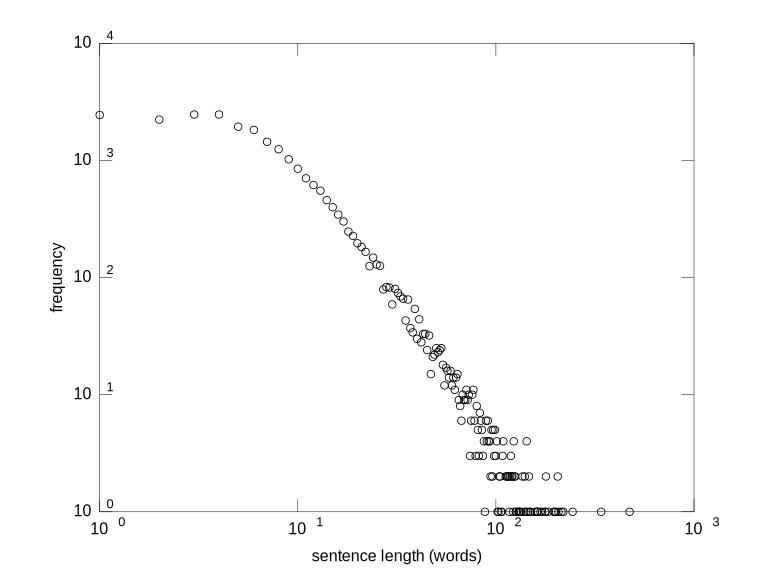
\includegraphics[width=0.75\textwidth]{images/ulysses_words_sentence_word_length_freq.pdf}
\caption{Frequency of occurrence of sentences for a given length.}
\label{fig:ulysses_words_sentence_word_length_freq}
\end{figure} 


Investigating the relation between sentences length and average words length, 
but this time, using the number of syllables as the unit to measure a word length,
we observe quite a different behavior, as it is presented in Figure \ref{fig:ulysses_words_sentence_word_length_syllables_z100}.
The analysis was again based on the text \textit{Ulysses}. Each word, in each sentence,
were transcribed into syllables using online dictionaries, and we considered only the sentences
where every word could be transcribed. The number of words and syllables in each sentence
was drawn, and the result is presented in Figure \ref{fig:ulysses_words_sentence_word_length_syllables_z100}.
The patter presented in that figure suggests a quantization effect of the size of half a syllable.
This might indicate that demi-syllables are actual constituent units of language, what would
corroborate the good achieved results in speech recognition systems using demi-syllables as 
the base unit \citep{yoshida1989}.

In speech recognition it is important to have a unit smaller than a word \citep{Shoup1988}. The demi-syllable is defined
as a half syllable, divided at the center of the syllable nucleus. This unit holds a transitional information,
which is important in the speech recognition task. It implicitly holds phonological constrictions, it is 
also suitable in size and can to take in account the co-articulatory effects.

\begin{figure}[h!]
\centering
\includegraphics[width=0.75\textwidth]{images/ulysses_words_sentence_word_length_syllables_z100.png}
\caption{Relation between sentences length (number of words) and the average word length (number of syllables a word is made of).}
\label{fig:ulysses_words_sentence_word_length_syllables_z100}
\end{figure} 



%
%
%
\section{Zipf Fit}
In the previous Chapter, we saw the Zipf plot of words, phones, diphones, triphones and syllables.
One way to compare the Zipf law for different data sources is to find the Zipf exponent that best
fits the given data. Once we have the model established and the data that we believe might be explained
by such model, we need a procedure to find the parameters that adjusts the best model for the given data.
There are two general methods for parameter estimation: least-squares estimation (LSE) and maximum likelihood 
estimation (MLE). The former is very popular and is tied to some familiar statistical concepts, such as linear
regression. LSE requires no distributional assumption on the data and is very helpful for obtaining a
descriptive model summarizing the observed data, but ``it has no basis for testing hypotheses or constructing
confidence intervals. (...) MLE has many optimal properties in estimation: sufficiency (complete information about 
the parameter of interest contained in its MLE estimator); consistency (true parameter value that generated the
data recovered asymptotically, i.e. for data of sufficiently large samples); efficiency (lowest-possible variance 
of parameter estimates achieved asymptotically); and parameterization invariance (same MLE solution obtained 
independent of the parametrization used). In contrast, no such things can be said about LSE.''\citep{myung2003}.

The Zipf model states that the probability of occurrence of samples is determined by a power law relation
and the rank of the each sample. Having defined the model, we want to find the population, defined
by a corresponding distribution, from which it is most likely that our observed samples would come from.
Associated with each population is a unique parameter for the model assumed. The Zipf model state that the 
probability density function (PDF) is defined by
\begin{equation}
\label{eq:zipf_relation}
f(k | s, N) = \frac{1/k^s}{\sum_{n=1}^{N} n^{-s}} = \frac{1/k^s}{H_{N,s}} ,
\end{equation} 
where $k$ is the rank of the observed samples, $s$ is the model parameter we want to determine,
and $N$ is the number of observations.
If individual observations are statistically independent one from another, then the PDF
of the set of observed data is equals to the product of all individual observations PDFs.
Suppose we have $M$ observations, then we will have the following probability
of experiencing this set of samples
\begin{eqnarray}
f(k=(k_1, k_2, \cdots, k_M) | s, N) &=& \prod_{m=1}^{M} f(k_m | s, N) \nonumber \\
		&=& \prod_{m=1}^{M} \frac{1}{k_m^s} \frac{1}{H_{N,s}} \nonumber \\
		&=& \left( \frac{1}{H_{N,s}} \right)^M \prod_{m=1}^{M} \frac{1}{k_m^s} .
\end{eqnarray}

Given a model and its parameters value, we might show that some data are more probable than others,
we appraise this through the PDF. As we are faced with the data and we want to find the model
that is the most probable to have generated that data, we are dealing with the inverse problem.
A \textit{likelihood function} is then defined by reversing the roles of the data and the parameters
in $f(k | s, N)$, i.e.
\begin{equation}
L(s | k, N) = f(k | s, N) .
\end{equation}
It represents the likelihood of the parameter $s$ given the observed data, and as such it is a function of $s$.

The Figure \ref{fig:zipf_likelihood_k} shows the likelihood function for some observations (some values of $k$, the rank).
As there are many observations, we conclude that the likelihood function which takes in account all
observations is the product of all the likelihood functions
\begin{eqnarray}
L(s|k_1,\cdots,k_M,N) &=& \prod_{m=1}^{M} L(s|k_m,N) \nonumber \\
          &=& \left( \frac{1}{H_{N,s}} \right)^M \prod_{m=1}^{M} \frac{1}{k_m^s} .
\end{eqnarray}
From a simple visual observation of Figure \ref{fig:zipf_likelihood_k} we may guess that the parameter $s$ that
gives the maximal likelihood for a set of observations might be somewhere in the interval $[1,2]$.

\begin{figure}[h!]
\centering
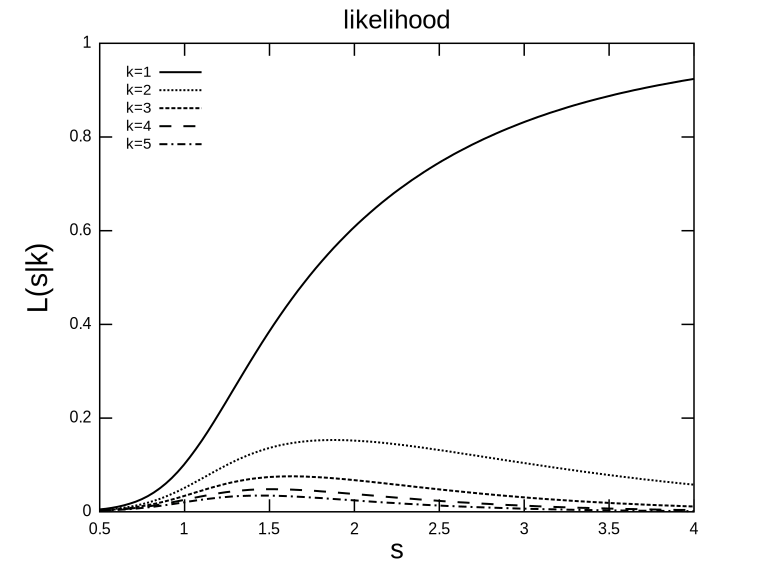
\includegraphics[width=0.75\textwidth]{images/zipf_likelihood_k.pdf}
\caption{Likelihood function for the Zipf model.}
\label{fig:zipf_likelihood_k}
\end{figure} 

The principle of maximum likelihood estimation (MLE) was introduced by \cite{fisher1922}, 
where he states that the desired probability distribution is the one that makes the observed data
most likely. The parameter that maximizes this likelihood function is the MLE estimate \citep{aldrich1997}.


The MLE estimate might not exist or even may not be unique. For computational convenience,
the MLE estimate $s_{\textmd{MLE}}$ is obtained by maximizing the log-likelihood function.
Assuming that $\ln L(s|k,N)$ is differentiable, the maximal value takes place when
\begin{equation}
\label{eq:dervloglikelihood}
\frac{\partial \ln L(s|k,N)}{\partial s} = 0 
\end{equation}
and when the second derivative is negative 
\begin{equation}
\frac{\partial^2 \ln L(s|k,N)}{\partial s^2} < 0 .
\end{equation}
The logarithm of the likelihood function is given by
\begin{equation}
\ln L(s|k_1,\cdots,k_M,N) = -M \ln H_{N,s} - s \sum_{m=1}^{M} \ln k_m .
\end{equation}
We need then to solve the equation \ref{eq:dervloglikelihood}. So we have to solve
\begin{eqnarray}
\label{eq:derivloglikeeqzero}
\frac{\partial \ln L(s|k_1,\cdots,k_M,N)}{\partial s} &=& - M \frac{d}{ds} \ln H_{N,s}  - \sum_{m=1}^{M} \ln k_m  \nonumber \\
	&=& -M \frac{1}{H_{N,s}} \frac{d}{ds} H_{N,s} - \sum_{m=1}^{M} \ln k_m  \nonumber \\
	&=& -M \frac{- \sum_{n=1}^{N} n^{-s} \ln n }{\sum_{n=1}^{N} n^{-s}} - \sum_{m=1}^{M} \ln k_m  \nonumber \\
	&=& -M \frac{G_{N,s}}{H_{N,s}} - \sum_{m=1}^{M} \ln k_m  = 0
\end{eqnarray}

We need to find $s$ that satisfies the equation \ref{eq:derivloglikeeqzero} and for which the second
derivative of the log-likelihood is negative. Taking the second derivative of the log-likelihood, we have
\begin{eqnarray}
\label{eq:d2dsloglike}
\frac{d^2}{ds^2} \ln L(s|k_1,\cdots,k_M,N) &=& \frac{d}{ds} \left( -M \frac{G_{N,s}}{H_{N,s}} \right) \nonumber \\
	&=& -M \frac{ \frac{d G_{N,s}}{ds} H_{N,s} - G_{N,s} \frac{d H_{N,s}}{ds} }{H_{N,s}^2} \nonumber \\
	&=& -M \frac{ \left( \sum_{n=1}^{N} n^{-s} \ln^2 n \right) H_{N,s} - G_{N,s}^2 } {H_{N,s}^2} \nonumber \\
	&=&  M \frac{  G_{N,s}^2 - I_{N,s} H_{N,s}  } {H_{N,s}^2}
\end{eqnarray}

The denominator in Equation \ref{eq:d2dsloglike} is always positive, so we need to verify if $I_{N,s} H_{N,s} \geq G_{N,s}^2$,
in order to make the second derivative negative.

We might then write
\begin{eqnarray}
\label{eq:GNs_cauchy}
G_{N,s}^2 &=&     \left( \sum_{n=1}^{N} n^{-s} \ln n  \right)^2 = \left( \sum_{n=1}^{N} n^{-s/2} (n^{-s/2} \ln n)  \right)^2 \nonumber \\
          &\leq&  \left( \sum_{n=1}^{N} \left( n^{-s/2} \right)^2 \right)    \left( \sum_{n=1}^{N} \left( n^{-s/2} \ln n \right)^2 \right) \nonumber \\
          &=& \left( \sum_{n=1}^{N} n^{-s} \right)    \left( \sum_{n=1}^{N} n^{-s} \ln^2 n \right) \nonumber \\
          &=&  H_{N,s}  I_{N,s} \textmd{ ,} 
\end{eqnarray}
where we have used the Cauchy-Schwarz inequality.


It has been proved that  $I_{N,s} H_{N,s} \geq G_{N,s}^2$ and therefore the second derivative of the likelihood function is always negative.
%As $n$ ranges from $1$ to $N$, only positive numbers, $\ln n$ and $n^{-s}$ will be positive for any $n$
%in the range, and for that reason $H_{N,s}$ , $G_{N,s}$ and $I_{N,s}$ are all positive numbers.
%The second derivative of the likelihood function is then always negative, and for that reason,
Any $s$ that satisfies equation \ref{eq:derivloglikeeqzero} is a maximum likelihood estimation.
We may use any root finding algorithm to find the MLE parameter of the Zipf model.

Figure \ref{fig:ulysses_fittedcurve_probabilities} presents some examples where we might observe that
the value of $s_{MLE}$ for a natural text is close and above $1$. All other random synthetic texts
present a $s_{MLE}$ whose value is bellow $1$. As the source characteristics approach a white random
source, the closer the estimated parameter gets to zero. A similar behavior might be observed 
when analyzing the entropy of the source. We shall see that the entropy increases as the characteristics
of the source approach a white random process.
Another aspect about the distinction on the model coefficient is important to note.
The value of $1$ seems to be a water shed between natural and random processes. 
From the Zipf relation in equation \ref{eq:zipf_relation} we might observe that for large extremely vocabularies
the value of the exponent must be above $1$ so that the normalizing coefficient $H_{N,s}$ converge.
$H_{N,s}$ is a Riemann zeta function which converges when the real part of the exponent $s$ is greater than $1$.

\begin{figure}
\centering
\begin{tabular}{cc}
  \subfloat[Natural text. $s_{MLE} = 1.0738$]{\label{fig:ulysses_fittedcurve_words_probabilities}\includegraphics[width=0.5\textwidth]{images/ulysses_fittedcurve_words_probabilities.png}} &
  \subfloat[Random text created by a Markov Model. $s_{MLE} = 0.95574$]{\label{fig:ulysses_fittedcurve_words_hmm_probabilities}\includegraphics[width=0.5\textwidth]{images/ulysses_fittedcurve_words_hmm_probabilities.png}} \\
  \subfloat[Random text with symbols weighted probabilities. $s_{MLE} = 0.84042$]{\label{fig:ulysses_fittedcurve_words_wrnd_probabilities}\includegraphics[width=0.5\textwidth]{images/ulysses_fittedcurve_words_wrnd_probabilities.png}}  &
  \subfloat[White random text. $s_{MLE} = 0.17076$]{\label{fig:ulysses_fittedcurve_words_rnd_probabilities}\includegraphics[width=0.5\textwidth]{images/ulysses_fittedcurve_words_rnd_probabilities.png}} 
\end{tabular}
\caption{Zipf plot of the frequency of occurrence of (pseudo)words and the fitted model.}\label{fig:ulysses_fittedcurve_probabilities}
\end{figure}








\subsection{Zipf-Mandelbrot Fit}
The same sort of procedure might be used to fit a Zipf-Mandelbrot model, given a set of observed values.
The Zipf-Mandelbrot distribution is given by
\begin{equation}
f(k | s, q, N) = \frac{1/(k+q)^s}{\sum_{n=1}^{N} (n+q)^{-s} } = \frac{1/(k+q)^s}{H_{N,s,q}}
\end{equation}
where $q$ denotes the flattening constant and $H_{N,s,q}$ is similar to the generalized harmonic number.

For a set of $M$ observations, $k_1, k_2, \ldots, k_m$, the likelihood function will be given by
\begin{equation}
L(s|k_1,\cdots,k_M,N) = \left( \frac{1}{H_{N,s,q}} \right)^M \prod_{m=1}^{M} \frac{1}{(k_m+q)^s} .
\end{equation}
and the logarithm of the likelihood is given by
\begin{equation}
\ln L(s|k_1,\cdots,k_M,N) = -M \ln H_{N,s,q} - s \sum_{m=1}^{M} \ln (k_m+q) \textmd{ .} 
\end{equation}
In order to find the maximum likelihood estimates for $s$ and $q$, we need to find 
\doubleequation[eq:dlnLds,eq:d2lnLds2]{\frac{\partial \ln L(s|k_1,\cdots,k_M,N)}{\partial s} = 0}{\frac{\partial^2 \ln L(s|k_1,\cdots,k_M,N)}{\partial s^2} < 0}
and
\doubleequation[eq:dlnLdq,eq:d2lnLdq2]{\frac{\partial \ln L(s|k_1,\cdots,k_M,N)}{\partial q} = 0}{\frac{\partial^2 \ln L(s|k_1,\cdots,k_M,N)}{\partial q^2} < 0 \textmd{ .}}


Lets first consider the parameter $s$. The partial derivative of the log likelihood in relation to $s$ is given  
\begin{eqnarray}
\label{eq:dlnLds1}
\frac{\partial \ln L(s|k_1,\cdots,k_M,N)}{\partial s} &=& -M \frac{1}{H_{N,s,q}} \frac{\partial H_{N,s,q}}{\partial s} - \sum_{m=1}^{M} \ln (k_m + q) \nonumber \\
          &=& -M \frac{1}{H_{N,s,q}} \frac{\partial}{\partial s} \sum_{n=1}^{N} (n+q)^{-s} - \sum_{m=1}^{M} \ln (k_m + q) \nonumber \\
          &=& -M \frac{1}{H_{N,s,q}} \left( -\sum_{n=1}^{N} (n+q)^{-s} \ln (n + q) \right) - \sum_{m=1}^{M} \ln (k_m + q) \nonumber \\
          &=& -M \frac{G_{N,s,q}}{H_{N,s,q}} - \sum_{m=1}^{M} \ln (k_m + q)
\end{eqnarray}
and the second derivative is given by
\begin{eqnarray}
\frac{\partial^2 \ln L(s|k_1,\cdots,k_M,N)}{\partial s^2} &=& -M \frac{\partial}{\partial s} \left( \frac{G_{N,s,q}}{H_{N,s,q}}  \right) \nonumber \\
          &=& -M \frac{\frac{\partial G_{N,s,q}}{\partial s} H_{N,s,q} - G_{N,s,q} \frac{\partial H_{N,s,q}}{\partial s}}{H_{N,s,q}^2} \nonumber \\
          &=& -M \frac{\left( -\sum_{n=1}^{N} (n+q)^{-s} \ln^2(n+q) \right) H_{N,s,q} - G_{N,s,q}^2}{H_{N,s,q}^2} \nonumber \\
          &=& M \frac{G_{N,s,q}^2 - I_{N,s,q} H_{N,s,q}}{H_{N,s,q}^2}
\end{eqnarray}
and it is shown as negative by following the same steps as in Equation \ref{eq:GNs_cauchy}.


Considering now the parameter $q$, we also need to calculate the first and second derivatives of the log likelihood in relation it.
The first derivative is given by
\begin{eqnarray}
\label{eq:dlnLdq1}
\frac{\partial \ln L(s|k_1,\cdots,k_M,N)}{\partial q} &=& -M \frac{1}{H_{N,s,q}} \frac{\partial}{\partial q} H_{N,s,q} - s \sum_{m=1}^{M} \frac{1}{k_m+q} \nonumber \\
          &=& Ms \frac{1}{H_{N,s,q}} \sum_{n=1}^{N} (n+q)^{-s-1} - s H_{N,1,q} \nonumber \\
          &=& sM \frac{H_{N,s+1,q}}{H_{N,s,q}} - s H_{N,1,q}
\end{eqnarray}
and the second derivative is given by
\begin{eqnarray}
\label{eq:dlnLdq21}
\frac{\partial^2 \ln L(s|k_1,\cdots,k_M,N)}{\partial q^2} &=& sM \frac{ \frac{\partial H_{N,s+1,q}}{\partial q} H_{N,s,q} - H_{N,s+1,q} \frac{\partial H_{N,s,q}}{\partial q} }{H_{N,s,q}^2} - s \frac{\partial}{\partial q} \sum_{n=1}^{N} (n+q)^{-1} \nonumber \\
          &=& sM \frac{ \left( \sum_{n=1}^{N} \frac{-s-1}{(n+q)^{s+2}} \right) H_{N,s,q} - H_{N,s+1,q}  \left( \sum_{n=1}^{N} \frac{-s}{(n+q)^{s+1}} \right)   }{H_{N,s,q}^2} + \ldots \nonumber \\ 
          && s \sum_{n=1}^{N} (n+q)^{-2} \nonumber \\
          &=& sM \frac{-(s+1) H_{N,s+2,q} H_{N,s,q} + s H_{N,s+1,q}^2}{H_{N,s,q}^2} + s H_{N,2,q} \nonumber \\
          &=& s^2 M \frac{H_{N,s+1,q}^2}{H_{N,s,q}^2} - s(s+1)M \frac{H_{N,s+2,q}}{H_{N,s,q}} + s H_{N,2,q} \textmd{ .}
\end{eqnarray}
The second derivate in relation to $q$ is also negative\footnote{This was not formally proved, but computation with various values of $s$, $q$ and $N$
indicates that it is indeed negative.}.


We conclude that the parameters that satisfies equations \ref{eq:dlnLds} and \ref{eq:d2lnLds2} for $s$ and 
equations \ref{eq:dlnLds} and \ref{eq:d2lnLds2} for $q$ are the maximum likelihood estimates for the 
Zipf-Mandelbrot model given the observed data. They might be found by any root-finding algorithm.











%
%
%
%
\section{Inverse Zipf}

% [25] G.K. Zipf, Psycho-Biology of Languages, Houghton-Mifflin, Boston, MA, 1935.

\cite{zipf1935} states the inverse law, which relates the number of words for a given frequency
to the frequency of occurrence by a power law function as described by the following equation 
\begin{equation}
N(f) = a f^{-b}
\end{equation}
where $N$ stands for the number of words with a given frequency $f$.
The constants $a$ and $b$ are parameters of the model. In the case of
natural texts, the value of $b$ is usually close to $2$.

% Inverse Zipf law has been used by Cohen et al.
% [26] and Ferrer and Solé [27] to study the properties of natural
% and random texts.
%[26] A. Cohen, R.N. Mantegna, S. Havlin, Numerical analysis of word frequencies in artificial and natural language texts, Fractals 5 (1) (1997) 95–104.
%[27] R. Ferrer i Cancho, R.V. Solé, Zipf’s law and random texts, Adv. Complex Syst. 5 (1) (2002) 1–6.


%
%The obvious estimator of the probability of the pair is r/N. This estimator is in
%fact the maximum likelihood estimator if the occurrence of the pair of interest is a
%random variable with a binomial distribution.
%
%

Imagine we have a large corpus where we might observe the occurrence of $M$ different words $W$.
The lexical described by this corpus is the set $\{W_1, W_2, \ldots, W_M\}$.
In this corpus we verify that each word presents a different frequency of occurrence,
that is described by $f_W$. The hypothetical frequency observed in a near-infinite corpus
is called the ``underlying frequency''. The simplest way to estimate the frequency of occurrence
is to count the number of occurrences and divide by the total counts. This estimator is
in fact the maximum likelihood estimator.
%if the occurrence of a word of interest is a random
%variable with a binomial distribution.
The probability of occurrence of a word is then given by
\begin{equation}
\label{eq:mle_prob}
p_W = \frac{f_W}{N}
\end{equation}
where $f_W$ is the count of occurrence for a given word $W$ and 
$N$ is the total number of words
in the corpus, $N = \sum_{m=1}^{M} f_{W_m}$. That would lead then to the satisfaction of the
relation $\sum p_W = 1$. But this cannot be, since, no matter how large the corpus is, there
will always be words with zero frequency in this corpus.

\begin{figure}[h!]
\centering
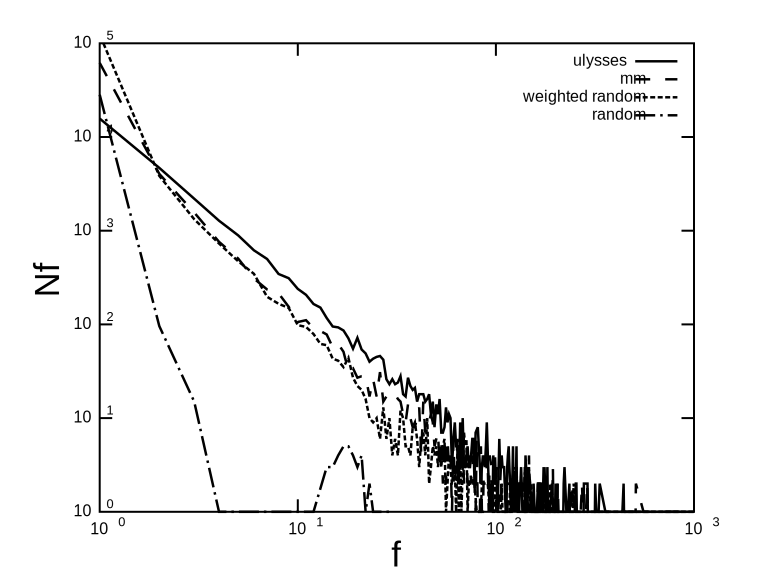
\includegraphics[width=0.75\textwidth]{images/inverse_zipf_ulysses_words.pdf}
\caption{Inverse Zipf plot applied to Ulysses data (words) and random generated words. The random texts
are created using the procedure as described before.}
\label{fig:inverse_zipf_ulysses_words}
\end{figure} 

The Figure \ref{fig:inverse_zipf_ulysses_words} presents the relation between the frequency of occurrence
of words $f$ and the number words which occur with that given frequency. We might observe that
words that happen few times are in a great number, and there are just a few words which are
very frequent. At high frequencies some gaps will emerge, that means there is no word with that
given frequency of occurrence. We might observe these gaps in the list of words and their frequency.
The most frequent word \textit{the} happens 15,126 times in \textit{Ulysses}; the next most frequent
word \textit{of} happens 8,256. There will be no word filling the gap between 15,126 and 8,256.
These gaps are also present in random generated text, but they are far less common.
Analyzing the texts in the example of Figure \ref{fig:inverse_zipf_ulysses_words}, we may
count the percentage of frequencies which present no occurring (pseudo-)words, the result is
50,8\%, 7,1\%, 3,5\% and 0,0\% for the natural text, markov model, weighted random and random generated
texts, respectively. The difference presented in the percentage of gaps is far too great. Another
observable difference is the steeper decay presented by the frequency of frequencies for the very low
frequency region of the random generated texts. For the rest of the frequency domain, we observe that
the frequency of frequencies of the natural text is always above the random text (excluding the gaps), what
might be explained as a compensatory effect of holding a large amount of gaps. 

It is important to note that, strictly when we talk about ``the frequency'', an assumption is made about
the random process which generate the observed data, we assume it does not change with time
nor depend on external events. When describing a language, these conditions are generally not considered,
and for that reason it would be more accurate to say ``the average frequency of occurrence of a word''.
We know that the frequency of occurrence of words change with time, for example, the frequency
of occurrence of \textit{throve} and \textit{thrived} changed in a 200 years gap causing the 
regularization of the verb \textit{thrive}. The change in the frequency of occurrence might also be
occasioned by external factors, for example, the frequency of occurrence the word \textit{influenza}
is influenced by the occurrence of epidemic flues \citep{baptiste2011}.





%%% calculate the exponent for the inverse Zipf
The word frequencies in human communications arrange themselves according to the Zipf's law.
This model has shown suitable for different languages \citep{naranan1996} with no exception found until now.
Although different functions have been proposed for modeling the word frequency relation \citep{tuldava1996},
the Zipf's law model still is argued as the best and most general model.
When we consider the frequency of frequency, we also observed a Zipf's law present in the Natural text.
If $P(f)$ is the probability of words with a given frequency $f$ in a corpus, we will observer a relation
\begin{equation}
\label{eq:freq_espec_prob}
P(f) \propto f^{-\beta}
\end{equation}
This exponent value is characteristic of the process under analysis. 
The relation in Equation \ref{eq:freq_espec_prob} might be interpreted as the frequency spectrum,
the value of $P(f)$ refers to the power spectral density related to the frequency $f$.
The value of $\beta=0$ characterize a white noise process ($1/f^0$); when $\beta=1$ the process is
characterized as a pink noise ($1/f$); and the value of  $\beta=2$ characterize a Brownian noise
or red noise process ($1/f^2$). Usually the value of $\beta$ approaches $1$, characterizing
a pink noise process \citep{mandelbrot1999}.

The Zipf'law relation presented in Equation \ref{eq:zipflaw}, states that $f \propto k^{-s}$, and from
this proportion we may also state that $k \propto f^{-1/s}$. From Equation \ref{eq:freq_espec_prob},
using the approach proposed by \cite{}, we may find another relation between rank and probability of
occurrence of a word. The number of words with a population $f$ in the sample is given by
\begin{equation}
m_f = T P(f)   \textmd{ , }
\end{equation} 
where $T$ is the total number of words in the sample. The rank a words with $f$ observations in the sample
is given by 
\begin{eqnarray}
\label{eq:rankprobfreq}
k(f) &=& \int_f^{\infty} m_{f'} df' \nonumber \\ 
     &=& \int_f^{\infty} T P(f') df' \nonumber \\
     &=& T C_p \int_f^{\infty} f'^{-\beta} df' \nonumber \\
     &=& T C_p f'^{(1-\beta)} \biggr|_f^\infty \textmd{ , }
\end{eqnarray}
where $C_p$ is the proportionality constant between $P(f)$ and $f$.
From Equation \ref{eq:rankprobfreq} we observe that $k \propto f^{(1-\beta)}$ and 
we may conclude that $f^{-1/s} \approx f^{(1-\beta)}$. There is then a relationship between the 
exponents
\begin{equation}
s = \frac{1}{\beta - 1} \quad  \textmd{ or } \quad \beta = \frac{1}{s} + 1 \textmd{ . }
\end{equation}

Natural languages typically present a value of $\beta \approx 2$ (or $s \approx 1$ by the relation above), 
but significant deviations from this typical value have been reported
in different contexts. \cite{piotrovskii} after analyzing various samples of schizophrenic language
have shown that a $\beta > 2$ is found in the fragmented discourse observed in schizophrenia.
The speech is marked by a multitude of topics with no consistent subject, resulting in a varied
and chaotic lexicon. In advanced forms of schizophrenia, \cite{piotrovskii} have found an exponent
$1 < \beta < 2$. The patients that suffer from this advanced form usually present obsessional topics
and the utterance construction is usually filled by words and compounds related to the topic.
Very young children present an exponent $\beta \approx 1.6$ \citep{piotrovskii} and older children conform to 
the typical $\beta \approx 2$ \citep{zipf1942}. \cite{kolguskin1960} showed that military combat texts present 
an exponent of $\beta = 1.7$. According to \cite{piotrovskii}, a larger value of the exponent $\beta \approx 2$
may be obtained as a result of deficient sampling from a text with the typical $\beta \approx 2$.

\cite{ferrer05} hypothesized that the variation observed in the exponent value $\beta$ ``reflects our ability 
to balance the goal of communication, i.e. maximizing the information transfer and the cost of communication, 
imposed by the limitations of the human brain''. The exponent value seems to be related to the 
communication efficiency, increasing the $\beta$ value leads to an increase in communicative efficiency. 
``This positive correlation is not easy to determine, because precise information theory measures, as far
as we know, have not been used for the atypical systems considered here'' \citep{ferrer05}.


\begin{figure}
\centering
\begin{tabular}{cc}
  \subfloat[Semantics: Cumulative frequency of occurrence of words with a given number of meanings.]{\label{fig:ulysses_words_semantic_sum_freq}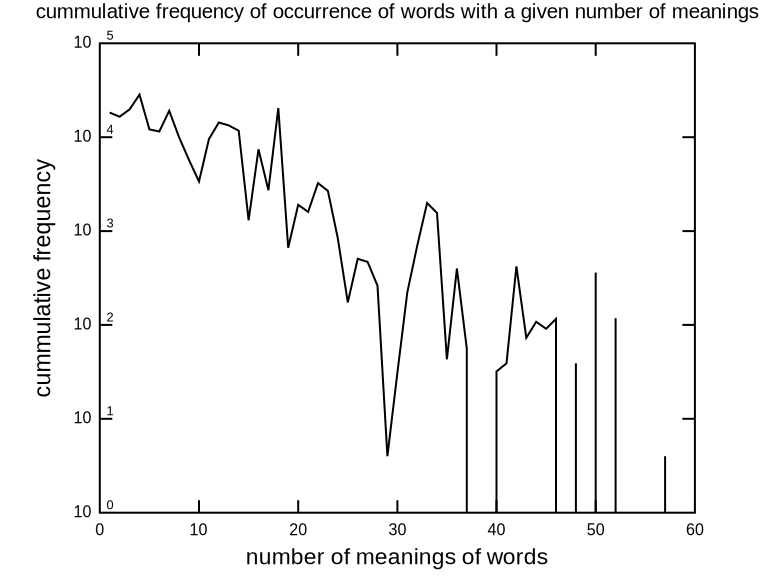
\includegraphics[width=0.45\textwidth]{images/ulysses_words_semantic_sum_freq.pdf}} &
  \subfloat[Syntax: Cumulative frequency of occurrence of words with a given number of syntactic functions.]{\label{fig:ulysses_words_syntatic_sum_freq}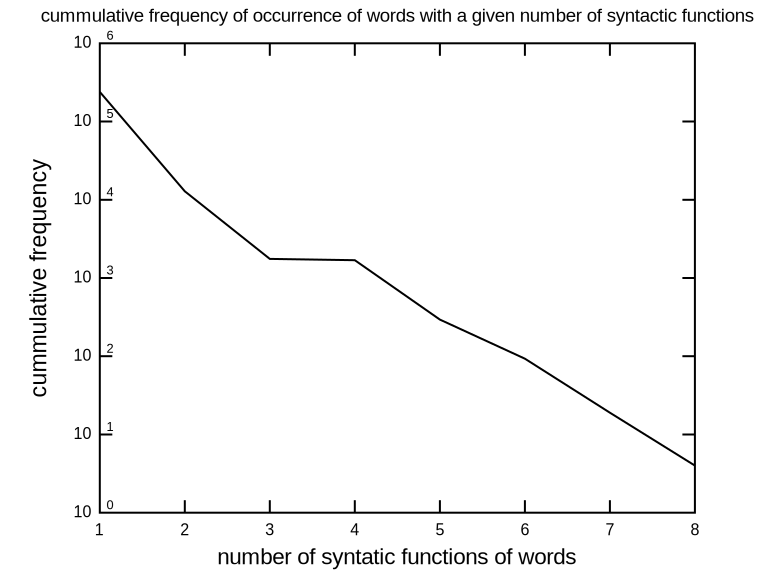
\includegraphics[width=0.45\textwidth]{images/ulysses_words_syntatic_sum_freq.pdf}}
\end{tabular}
\caption{For both pictures the frequency of occurrence data comes from the text \textit{Ulysses}. They present the cumulative frequency of occurrence of words for a certain number of meanings and syntactic functions.}
\label{fig:ulysses_comes}
\end{figure}













\section{Smoothing}
The estimation of the probability of a word given in Equation \ref{eq:mle_prob} is the MLE.
The problem with the MLE is that it predicts that the probability of a word not seen in the corpus
is zero. That might be a problem when trying to use the counts in one corpus to estimate what will
be seen in another corpus. A language with lots of rare words might suffer with this, especially
when the selected corpus does not comprise a fraction of these words. In order to take in account 
the existence of theses words that were not present in the corpus at hand, we need to make some 
considerations. 
A common approach is to add small positive quantities to all events, including the unobserved events. 
This technique was advocated by \cite{Lidstone1920, Johnson1932,jeffreys1939theory}.
When this additive method is applied adding one to every event, is known as the \textit{Add-One} estimator.
This is an obvious and simple approach, which was proposed by \cite{laplace}, 
but it lacks a principled justification and may lead to
inaccurate estimates.
\cite{Gale94} investigated the \textit{Add-One} in detail and concluded that it may give approximately
accurate estimates only for data-set which obey certain quite implausible numerical constraints:
``for Add-One to produce reasonable estimates, it is necessary that the ratio of unseen types to
observed types and the ratio of all types to the training sample size be equal. Since there is no reason for a
relationship between sample size and the population surveyed, this condition is usually invalid'' \citep{Gale94}.


A better approach was worked out by Alan Turing and his statistical assistant 
Irving John Good during their effort in the Second World War to crack the German ciphers for the Enigma machine.
Their approach was theoretically well-founded and are proven to perform well.
The Good-Turing estimator \citep{Good1953} considers that the unseen events
together have a probability equal to the sum of the probabilities of all events that were observed
only once in the corpus, for they are equally rare, and the fact that one was present in the corpus
and the other not is just a mere question of chance.
The method proposed by \cite{Good1953} results from an empirical use of Bayes formalism
and it can be obtained by significantly different statistical methods. Three examples of derivation
of Good's formula are compared by \cite{nadas1985}.


These techniques here analyzed are called \emph{smoothing}. They are used to adjust the maximum 
likelihood estimates of probabilities to achieve a better estimate when there is insufficient data to 
approximate them accurately. ``The name \emph{smoothing} comes from the fact that these techniques
tend to make distributions more uniform, by adjusting low probabilities such as zero probabilities
upward, and high probabilities downward. Not only do smoothing methods generally prevent zero
probabilities, but they also attempt to improve the accuracy of the model as a whole. Whenever
a probability is estimated from few counts, smoothing has the potential to significantly improve
estimation'' \citep{chen98}.
 


Many linguistic phenomena exist in an infinite multitude of different types. Words and sequences of words
are essentially infinite in number, i.e, in any finite amount of text of speech sample, we expect
to see words and sequences that were not seen before. It is important to have a good statistical estimate
of the occurrence of such types in order to increase the performance of systems that perform tasks such as 
spelling correction, sense disambiguation and machine translation. For good operation of those systems 
it is important that the probability of occurrence of unseen events are not estimated as zero.

The frequency of occurrence of words with a given frequency also present a Zipf-like relation.
There are few very frequent words, and their frequency of occurrence differ in great magnitude.
On the other hand, there are a lot of words which happen just once or twice in a language corpus.
If we plot the relation between the number of words that occur with a certain frequency
of occurrence, we shall realize that the relation is given by a power law, that might be 
observed as a straight line in a log-log plot. This type of analysis is also called 
\textit{inverse Zipf}.


When analyzing the frequency of occurrence of frequencies of words in a language, we have not only to 
deal with the zero created by those words that never happened, but also the zeros created by the gaps
that usually exist in the high frequency region. Suppose that in our toy-corpus the most frequent word
\textit{the} has a frequency of occurrence equals to 265,470, and the second most frequent word \textit{of}
has a frequency of occurrence equals to 187,168. If we count the number of words that occurred 265,470 times
in the corpus, it will be only one, \textit{the}. There will be no word which occurred 265,469 times,
nor 265,471 times, we might conclude that the number of words which have a frequency of occurrence 
from 265,469 to 187,169 will be zero, and the same happens for words with a frequency of occurrence above 265,470. 
It seems reasonable to imagine that the word \textit{the} could have
happened 265,471 times or 265,469 times or any other number around the actual value found in the corpus.
It is desired then to consider that the probability of occurrence of words
with frequency 265,471, 265,469, etc. is not zero. On the other extreme, we shall observe a large number of
words that occur only once, and a smaller number of words that occur twice, and so on. 
Observing the number of words for a given frequency of occurrence, we expect to experience a monotonically
decreasing number of words as the frequency of occurrence increases. 

In our toy-corpus example, we might suppose that words like \textit{obliteration}, \textit{freckles} and 
\textit{apotheosis} happen only twice, and words like \textit{headroom}, \textit{smugness} and \textit{hazelwood} 
happen just once. Adding up all words with just one occurrence, we get the total of 4,812. The
observed number of words whose frequency of occurrence is two is 2,345.
We shall use the notation $N_f$ to indicate the number of occurrence of words with a given frequency 
(the frequency of frequency). In our example above, we have $N_{265,470} = 1$, $N_{265,469} = 0$, 
$N_{265,468} = 0$, $N_{187,168} = 1$, 
$N_{2} = 2,345$ and $N_{1} = 4,812$. The total number of tokens observed in our corpus might
be calculated by
\begin{equation}
N = \sum_{f} f N_f
\end{equation}

Good-Turing methodology estimate that the total probability of all unseen events is equal to the 
sum of probabilities of all events that occur only once ($N_0 = N_1$), that gives the following
probability for the unseen events
\begin{equation}
p_0 = \frac{N_1}{N}
\end{equation}
We denote here by $p_f$ the probability of events that are observed $f$ times. 
Using the MLE the estimate, the events not observed have $p_0 = 0$. As we have stated before,
we want methods which give an estimate for $p_0$ which exceeds zero, as is the case for
the Good-Turing estimate, which will give the value $p_0 = N_0 / N > 0$.

The Good-Turing method \citep{Good1953} defines $N_f^\ast$ to be such that $p_f \equiv N_f^\ast / N$.
In the MLE, we have $N_f^\ast = N_f$. The values of $N_f^\ast$ for $f \geq 1$ must
be chosen so that the sum of all probabilities is equals to one: 
\begin{equation}
\label{eq:sum_pro_add_one}
\sum_f p_f = 1
\end{equation}
We must then reduce the probability of the seen events in order to take in account
the probability of the unseen events, in such a form that equation \ref{eq:sum_pro_add_one}
is still true. The Good-Turing method states that
\begin{equation}
\label{eq:goodturingnormnum}
f^\ast = (f + 1) \frac{E[N_{f+1}]}{E[N_f]}
\end{equation}
where $E[\cdot]$ represents the expectation of a random variable.
$f^\ast$ is usually called the ``adjusted number of observations'', that
represents how many words you are expected to see with a given frequency of occurrence.
The probability of the unseen events will be approximated by $E[N_1]/N$.
The value of $N_1$ is the largest value and the best estimate among all others $N_f$.
For that reason, to use the value of $N_1$ is a good approximation to the value of $E[N_1]$.


The Good-Turing estimate is a central procedure for other smoothing techniques. To derive the
estimate proposed in Equation \ref{eq:goodturingnormnum}, let assume there are $s$ different types
$\alpha_1, \alpha_2, \ldots, \alpha_s$ and that their underlying probabilities are respectively
$p_1, p_2, \ldots, p_s$.  We might estimate the probability of a type given we know how many
occurrences of that type exists on our sample. It will be expressed by $E[p_i | c(\alpha_i) = f]$,
where $E[\cdot]$ denotes the expected value and $c(\alpha_i)$ denotes the number of times the
type $\alpha_i$ has occurred on the given data. The expected value given above might
be expanded as
\begin{equation}
\label{eq:Epicif}
E[p_i | c(\alpha_i) = f] = \sum_{j=1}^{s} p(i=j | c(\alpha_i) = f) p_j
\end{equation}
where $p(i=j | c(\alpha_i) = f)$ is the probability that the unknown type $\alpha_i$, with $f$ occurrences
in the sample, actually is the $j$th type with underlying probability $p_j$. The probability
$p(i=j | c(\alpha_i) = f)$ might be written as the probability that the type $\alpha_j$ appears $f$
times in the data divided by the sum of the probabilities for all types.
\begin{eqnarray}
\label{eq:pijcif}
p(i=j | c(\alpha_i) = f) &=& \frac{p(c(\alpha_j) = f)}{\sum_{j=1}^{s} p(c(\alpha_j) = f)} \nonumber \\
         &=& \frac{ {N \choose f} p_j^f (1-p_j)^{N-f} }{ \sum_{j=1}^{s} {N \choose f} p_j^r (1-p_j)^{N-f} }  \nonumber \\
         &=& \frac{ p_j^f (1-p_j)^{N-f} }{ \sum_{j=1}^{s} p_j^f (1-p_j)^{N-f} }
\end{eqnarray}
where $N$ is the total number of counts (tokens) in the sample, what might written as $N = \sum_{j=1}^{s} c(\alpha_j)$.

Substituting the result from Equation \ref{eq:pijcif} in Equation \ref{eq:Epicif} we get
\begin{equation}
\label{eq:Epicif}
E[p_i | c(\alpha_i) = f] = \frac{ \sum_{j=1}^{s} p_j^f (1-p_j)^{N-f} }{ \sum_{j=1}^{s} p_j^f (1-p_j)^{N-f} } \textmd{ .}
\end{equation} 

Consider now $E_N [n_f]$ the expected number of types which present $f$ counts in a sample of size $N$.
This is equal to the sum of the probability that each type has exactly $f$ counts
\begin{equation}
\label{eq:ENnf}
E_N [n_f] = \sum_{j=1}^{s} p( c(\alpha_j) = f ) = \sum_{j=1}^{s} {N \choose f} p_j^f (1-p_j)^{N-f} \textmd{ .}
\end{equation}
Using Equation \ref{eq:ENnf} in Equation \ref{eq:Epicif} we may write
\begin{equation}
\label{eq:Epicif}
E[p_i | c(\alpha_i) = f] = \frac{f+1}{N+1} \frac{E_{N+1} [n_{f+1}]}{E_N [n_f]} \textmd{ .}
\end{equation}
We have just found an estimate for the expected probability of a type $\alpha_i$ with $f$ counts.
The Good-Turing probability based on the correct count value is given by
\begin{equation}
\label{eq:pGT}
p_{GT} (\alpha) = \frac{f^\ast}{N} \textmd{ .}
\end{equation}
Using Equation \ref{eq:pGT} in conjunction with Equation \ref{eq:Epicif} we may write the corrected 
counting value as
\begin{equation}
\label{eq:fastNf1N1}
f^\ast = N \frac{f+1}{N+1} \frac{E_{N+1} [n_{f+1}]}{E_N [n_f]} \approx (f+1) \frac{n_{f+1}}{n_f} \textmd{ ,}
\end{equation}
where we have used the following approximations $N/(N+1) \approx 1$, $E_N [n_f] \approx n_f$ and
$E_{N+1} [n_{f+1}] \approx n_{f+1}$. The empirical values of $n_f$ are used to estimate their expected values.

One problem with the Good-Turing estimation is that it cannot be used when $n_f = 0$, what unfortunately
is really common for high values of $f$. \cite{galesampson95} propose a smoothing method, based on
Good-Turing, which overcomes this difficulty.


\subsection{Simple Good-Turing}

A simple way to do a Good-Turing estimation \citep{galesampson95} is to choose a $E[\cdot]$ so that
\begin{equation}
\label{eq:goodturingestimator}
E[N_{f+1}] = E[N_f] \left( \frac{f}{f+1} \right) \left( 1 - \frac{E[N_1]}{N} \right)
\end{equation}
Using the relation \ref{eq:goodturingestimator} and \ref{eq:goodturingnormnum}, 
the probability of occurrence of words with a given frequency $f$
will be given by
\begin{eqnarray}
p^\ast_f &=& \frac{f^\ast N_f^\ast}{N} \nonumber \\
    &=& \frac{(f+1) N_f E[N_{f+1}]}{N E[N_f]} \nonumber \\
    &=& \frac{(f+1) N_f E[N_f] \frac{f}{f+1} \left( 1 - \frac{E[N_1]}{N} \right)}{N E[N_f]} \nonumber \\
    &=& \frac{f N_f}{N} \left( 1 - \frac{E[N_1]}{N} \right) \nonumber \\
    &=& p_f \left( 1 - \frac{E[N_1]}{N} \right)
\end{eqnarray}
It means that the new estimated probability of a given type, if the sample were
perfectly representative of the population, is given by the previous probability,
which regards only the observed samples, multiplied by a factor to take in account 
the unseen types.
This relation means to scale down the maximum likelihood estimator $f N_f/N$ by a factor of $(1 - E[N_1]/N)$.
If we sum all $p^\ast_f$ for every seen word in the corpus we get
\begin{eqnarray}
\sum_f p^\ast_f &=& \sum_f \frac{f N_f}{N} \left( 1 - \frac{E[N_1]}{N} \right) \nonumber \\
           &=& \frac{1}{N} \left( 1 - \frac{E[N_1]}{N} \right) \sum_f f N_f \nonumber \\
           &=& \left( 1 - \frac{E[N_1]}{N} \right)
\end{eqnarray}
since $\sum_f N_f$ for the seen words is exactly $N$. The result given above agrees with
what we have specified before, that the probability of unseen words would be $E_1/N$,
adding the probability of all words (seen and unseen) we get $1$ as result. 

In the method propose in Equation \ref{eq:goodturingestimator}, we need the value of 
$f+1$ to make the new estimation $E[N_{f+1}]$. Unfortunately, as we move forward
increasing the value of $f$ we are going to find some gaps, and large gaps
in the region of high values of $f$. Those gaps are zeros, and for that reason
the equation \ref{eq:goodturingestimator} should not be applied to estate those estimates.
A modified version of the presented method, called the Simple Good-Turing method (SGT) \citep{gale1994},
states that, for these point where zeros were found, we should use instead the best fit power law
to approximate these values of $f$.

In order to do so, a new variable $Z_f$ is defined as 
\begin{equation}
Z_f = \frac{2 N_f}{f'' - f'}
\end{equation}
where $f'$ is the nearest lower sample frequency and $f''$ is the nearest higher sample frequency
such that $N_{f'}$ and $N_{f''}$ are both nonzero.
The log-log plot of $f$ and $Z_f$ typically shows a linear trend, and for that reason a straight line
is used as the simplest possible smoothing. A least squared error method is then used to fit the best
line. A criteria is used to select whether to use the new approximation $f^\ast$ or the liner fit
approximation. This criteria is based on the standard deviation on the estimate based on $N_f$.
The pair of $f^\ast$ estimates may be considered significantly different if their difference exceeds
1.96 times the standard deviation (the square root of the variance). 
``Assuming a Gaussian distribution of the estimate, the probability of
such a difference occurring by chance is less than the accepted .05 significance criteria. (...)
It is the adoption of a rule for switching between smoothed and raw frequencies of frequencies which
allows the SGT method to use such a simple smoothing technique. Good-Turing methods described previously
have relied on smoothed proxies for all values of $f$, and this has forced them to use smoothing calculations
which are far more daunting than that of SGT'' \citep{galesampson95}.
The variance for the Turing estimate is approximately
\begin{equation}
Var(f^\ast_T) \approx (f+1)^2 \frac{N_{f+1}}{N_f^2} \left( 1 + \frac{N_{f+1}}{N_f} \right)
\end{equation}



Any method of smoothing data must satisfy certain prior expectations about $f^\ast$. First we expect that
$f^\ast$ will be less than $f$, for all nonzero values of $f$; and second, we expect the ratio $f^\ast/f$
to approach unity as $f$ increases. An example is shown in Figure \ref{fig:simplegoodturing_ulysses_words} where the corpus used was the 
text \textit{Ulysses} by James Joyce. In this example $f$ is the frequency of occurrence of words
and $N_f$ is the number of words (types) that present $f$ occurrences (tokens) in the corpus.
We might observe that the smoothed version present a smaller value of $f^\ast$ and the ration
$f^\ast/f$ approaches unity as $f$ increases, since the larger $f$ is, the better it is measured,
and for that reason $f^\ast$ should be closer to $f$, compared to lower values of $f$.


%\begin{figure}[h!]
%\centering
%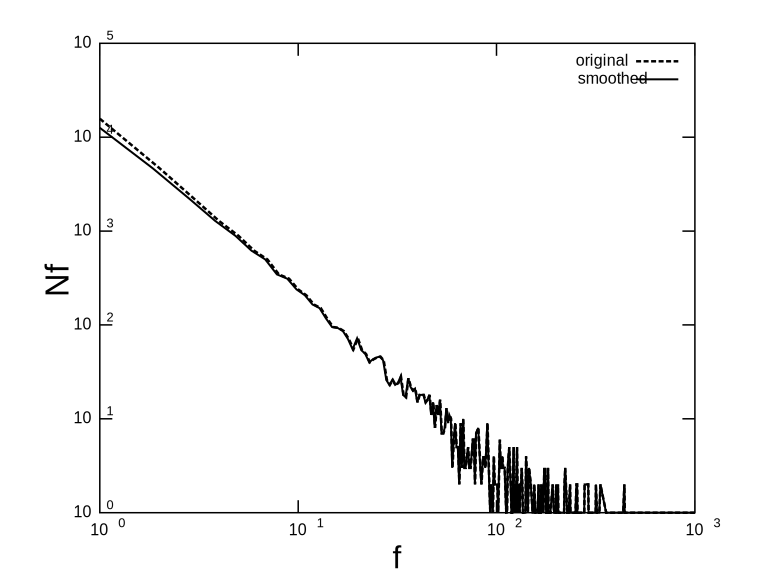
\includegraphics[width=0.75\textwidth]{images/simplegoodturing_ulysses_words.pdf}
%\caption{Simple Good-Turing Smoothing applied to Ulysses data (words).}
%\label{fig:simplegoodturing_ulysses_words}
%\end{figure} 

\begin{figure}
\centering
\begin{tabular}{cc}
  \subfloat[Zipf plot]{\label{fig:zipfplot_original_sgt}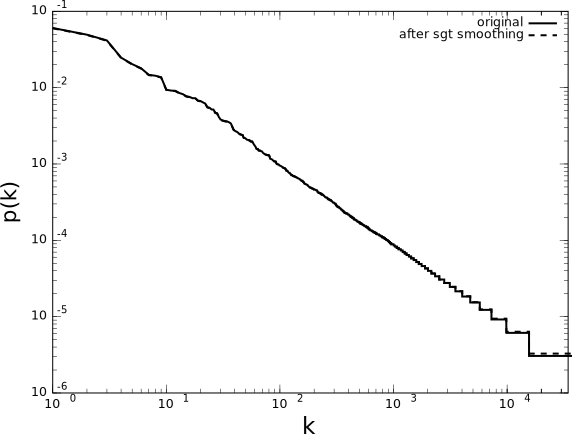
\includegraphics[width=0.45\textwidth]{images/zipfplot_original_sgt.pdf}} &
  \subfloat[Inverse Zipf plot]{\label{fig:inverseZipfplot_original_sgt}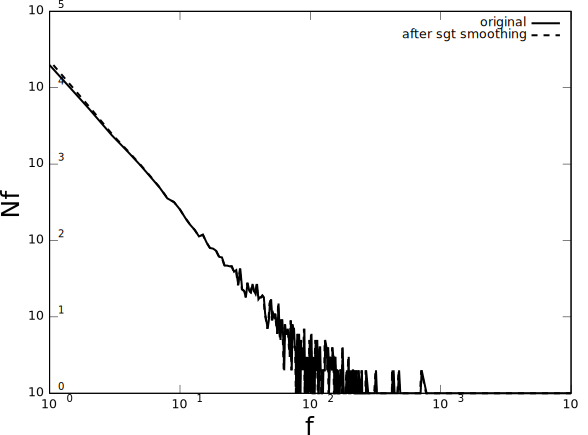
\includegraphics[width=0.45\textwidth]{images/inverseZipfplot_original_sgt.pdf}}
\end{tabular}
\caption{Simple Good-Turing Smoothing applied to Ulysses data (words).}
\label{fig:simplegoodturing_ulysses_words}
\end{figure}



The smoothing procedure defined by the SGT method presuppose that all unseen objects
together amount a frequency of occurrence of those objects seen once.
If we decide to divide this probability equally amount the unseen objects,
it requires to rely on an assumption over the structure of the objects, and that
decision might depend on the application at hand.
\cite{gale1991} show one example using bigram of pair of words where they use 
two alternative methods, one of them is an enhanced version of the Good-Turing method
using ``the modest assumption that the distribution of each bigram is binomial''\citep{gale1991}.
The methods analyzed use a second predictor of the probability in addition to the observed
frequency, making it possible to estimate different probabilities for bigrams with the
same frequency (that is the reason the method is known as an \textit{enhanced} Good-Turing method).

\cite{samuelsson1996} presents the relation between Turing's smoothing formula
and Zipf's law, using an asymptotic approximation for population frequencies
derived from Turing's formula and a local reestimation formula derived from 
Zipf's law. The two are shown to be instances from a common class of reestimation-formula,
although they are qualitatively different. The Turing's formula is shown to ``smooths
the frequency estimates towards a geometric distribution. (...) Although the two equations  
are similar, Turing's formula shifts the frequency mass towards more frequent species.''. 











\section{Information}
The main concern in communication is delivering a message containing information.
This process involves always a sender and a receiver, and it requires certain agreements 
between the parts. If the message is misunderstood at the receiving end, the communication process failures.
In every communication the transmitted information is \textit{a prior} unknown, and therefore there might
always be doubt if the information extracted from the received message corresponds to the correct 
information the sender meant to send. The study of the communication process and the effective transmission
of information is the main motivation in Information Theory.

In a communication process there are at least two participants which are physically apart. 
The information must somehow pass through the surrounding medium to achieve its goal. For that reason
it must be modulated appropriately. The modulation used is intrinsically linked to the medium 
and its properties.
The modulated message is an representation of the primary information into another form which is
suitable to the communication process across the surround medium.
In a speech communication process, the speaker is the source that produces a message which is 
intended to be received by a listener. The information to be sent is modulated into an utterance
which travels through the air medium as a acoustic wave and is further perceived by the listener.
To achieve communication successfully, it is necessary that both speaker and listener share
the same code.

\begin{figure}[htbp]
\centering
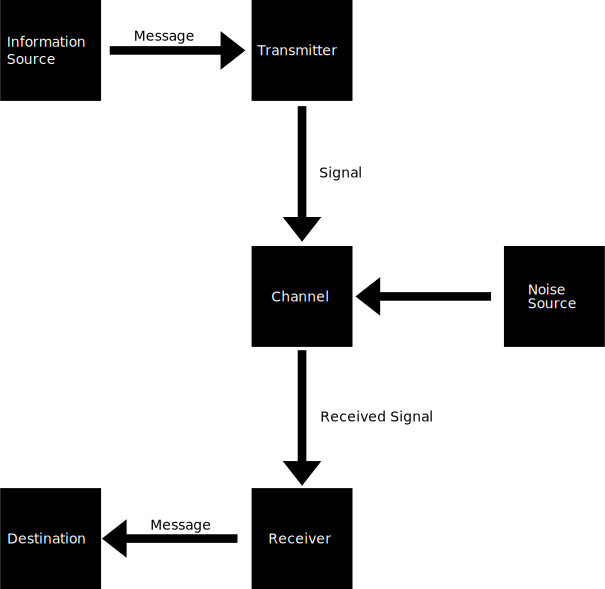
\includegraphics[width=0.5\textwidth]{images/communication_system.pdf}
\caption{Schematics of a Communication System}
\label{fig:communication_system}
\end{figure}  

The information is coded through signs, which are representations of symbols. The study of 
information by the \textit{Information Theory} has a postulate that it might be represented
by a set or sequence of symbols, and symbols are discrete in nature. What is perceived
by the receptor are just signs of the coded information. The discreteness feature is very important,
it makes the whole system operates in a discrete set 
%built upon also discrete 
and that makes it possible to undertake corrections 
when a signal is distorted. The communication is always degraded by environmental noise, so distortion 
is inevitable. To achieve good communication it is desired a that system has correction capabilities.

If the set of symbols is finite, and also the duration of any message, we may conclude that each message may
be represented by a finite subset of symbols, and coded in a finite time. 
The cardinality of the set is determined
by the coding process, the symbols used and the complexity of the information conveyed.

One coded message to be transmitted through a communication system is one 
selected from a set of many possible combinations of symbols. 
%One significant aspect is that one certain coded message to be transmitted through a communication system is,
%in fact, one selected from a set of possible combination of symbols, regarding to the many restrictions
%that might be imposed to the creation of such messages. 
Concerning a measure of the information in a message, 
Shannon pointed out: ``If the number of messages in the set is finite then this number or any monotonic function
of this number can be regarded as a measure of the information produced when one message is chosen from the set,
all choices being equally likely''\citep{shannon1948}. 
The use of a logarithmic function for measuring information
was proposed by Hartley \citep{hartley1928} in 1928 and is more convenient for various reasons: 
linear variation with the logarithm of the number of possibilities; 
resemblance to our intuitive feeling of a measure of information 
(two memory cards have twice the capacity of information storage of one memory card; and 
two communication channels have twice the capacity of transmitting information compared to one single channel); 
it is mathematically more suitable.

Figure \ref{fig:communication_system} depicts a schematics of a generic communication system. 
This representation comprises 6 basic blocks. 
The `information source' is the one which produces a message to be transmitted. 
This message, which conveys information, may be of many sorts, according to the problem at hand. 
If we are analyzing a telegraph system, we consider a sequence of letters as the message 
%with the information 
to be transmitted; 
in a speech conversation, we may consider 
%the message to be transmitted as 
a sequence of words, 
representing the message that conveys information; 
in a radio transmission, the message is a function of time $f(t)$
which express the acoustic signal that carries music or speech content. 
%Of course, we are considering a part of the whole problem, we are taking in assumption that this function 
%in time is our source of information, we have no concern how it was generated, what sort of information 
%does it carry and how it all works, because in this example we are analyzing the radio broadcasting as 
%the communication system, and not the human being speaking or singing in the microphone, nor the guitarist 
%pulling the strings on his guitar. 
The second block is the `transmitter', which is responsible for coding the input message 
into some sort of signal that will be suitable for transmission over the channel. 
In the telegraphic example, the transmitter is responsible in converting the letters sequence 
into a sequence of dots, dashes and spaces. In the speech communication, the transmitter is responsible 
for coding and producing a signal by means of articulation of the oral tract. 
In the radio transmission example, the transmitter performs the FM modulation on the signal, so that the information 
of $f(t)$ will now be represented by a modulation in frequency of a carrier. 
The next stage in the communication system is the channel. 
At this stage we may not control all the pertaining conditions as desired to a successful communication. 
The channel is indeed the medium where the signal will be transmitted. It may be a pair of wires, 
as in the telegraphic example, or the free air, as in the speech communication example and the radio broadcast example. 
The channel is then susceptible to noise, that means the signal may be corrupted by other undesirable sources. 
The pair of wires is susceptible to induced electrical field from other sources in the surrounding, 
it is susceptible to thermal noise, caused by natural random movements of the free electrons in a conductor. 
The free air is susceptible to climatic variations and also to many other sources that also use this medium for 
communication, in the speech communication example we have the popular `cocktail party' example. 
The transmitted signal travels all the medium from the transmitter until reaching the `receiver', as a final destination. 
The receiver has to do exactly the opposite done by the transmitter. The receiver attempts to reconstruct the transmitted
message, performing the decoding process and corrections when necessary. In the `cocktail party' example, we know from 
experience that corrections do actually occur. In such loud conditions, we may understand everything someone says although 
the signal received is heavily corrupted. Finally, the message reaches the destination, where the information received will 
be interpreted, and the communication process is then finished.


\subsection{The Measurement of Information}
A quantitative measure of information was proposed by \citep{hartley1928}, contrasting physical aspects with 
psychological considerations. The term information is very elastic and it is necessary to define a specific 
meaning of it. Weather dealing with transmission or storage of information, in our discussion we may consider 
it in terms of a selection from a group of physical symbols, such as words, phonemes, dots and dashes, 
which under certain agreement convey certain messages to the communicating parties.

During the communication process, the sender, according to the message (s)he is willing to transmit, 
selects symbols successively from the symbols inventory. The realization of those symbols is transmitted and 
received at the other side. The receiver, by means of the receiving signal and through successive selections, 
has brought to attention a set of symbols, eliminating many other possibilities of what could be the ordered 
set of symbols received. As the communication process proceeds, more symbols are received, and more possible 
ordered set of symbols are eliminated, making information more precise.

The precision of information depends not only on what was the set of symbols transmitted, 
but also on what it could be. For example, consider two sentences and their respective informations: 
`I bought a red car' and `I bought a red apple'. The information conveyed by the word `red' in both sentences 
is complete disparate. On the first sentence `red' specify a quality among a great set of possibilities. 
On the second sentence, there are only two possibilities (`red' or `green'), so the information added 
by the word `red' does not convey as much information as in the first example. 
Of course, this statement is true only when the communication parties share the same knowledge that 
apples can only be red or green. We may conclude that the degree of information depends also on the 
previous understanding on available symbols existing between the communicating parties.

In every communication system, the receiving signal can differ many degrees from the transmitted signal. 
The corruption of signals is a natural phenomena every communication system is susceptible to. 
The traveling signal may be weakened and degraded by noise. When this signal arrives at the receiver it 
may not be recognized at all or miss-recognized. The ability of the receiver to detect and correct errors 
in the incoming signal is of great importance to the effective characterization of information.

Considering a system where there are $7$ symbols available, the selection of two symbols makes 
possible $7^2$ (or $49$) different permutations, the selection of three makes $7^3$ (or $343$) possibilities 
and the selection of $n$ makes $7^n$. If we have a system with $s$ different symbols available to selection, 
it makes a total of $s^n$ permutation possibilities when considering a process of $n$ choices in this system.
If we consider now an example where we have two system with different symbol repertories. 
The first system has $s_1$ symbols and the second system $s_2$ on their repertories, respectively. 
The second system's work is to gather $n_1$ symbols emitted by the first system and assign to each set of symbols 
a new symbol from the second system's repertory. We may conclude that the size of the second system's repertory 
must be at least the total number of possible permutations of $n_1$ symbols from the first system, 
and we may chose the lowest available value, because it has no sense to keep unused symbols in our repertory. 
The number of symbols in the second system's repertory is $s_2 = s_1^{n_1}$. After a communication process proceeds 
that the second system has transmitted $n_2$ symbols, leading to $s_2^{n_2}$ choices in that system. 
If we consider the system that works on the primary symbols, the number of observed symbols will be $n_2 n_1$ symbols. 
An amount of $n_2 n_1$ symbols is capable of creating $s_1^{n_2 n_1}$ permutations, when working with the first symbol
repertory, what must be equivalent to the number of choices of the system using the second repertory: 
$s_1^{n_1 n_2} = s_2^{n_2}$.

A system with a repertory of $s$ symbols is capable of creating $s^n$ different sequences of symbols when faced 
with $n$ choices. If we consider the number of different permutations as a measure of information, 
we would have a exponentially increasing number. Each new symbols added to a sequence would add much more information 
than the previous ones. That seems contra-intuitive. It would be a more reasonable measure of information, 
some sort of measure that is proportional to the number of choices and not to the number of possible permutations. 
The information associated with $n$ selections is given then by
\begin{equation}
H = K n \textmd{ .}
\label{eq:HKn}
\end{equation}
The constant $K$ depends on the number of symbols $s$, because the information conveyed by a single choice is a 
function of the number of possibilities in this choice.

Comparing two system with $s_1$ and $s_2$ number of symbols in inventory, and constants $K_1$ and $K_2$, 
respectively associated with them, we may define both constants in such a way that the amount of information on 
both system is the same, $H=K_1 n_1 = K_2 n_2$, when the number of selections associated with each one is the same,
$s_1^{n_1} = s_2^{n_2}$. Taking this assumption we conclude that
\begin{equation}
\frac{K_1}{\log s_1} = \frac{K_2}{\log s_2} \textmd{ .}
\end{equation}
This relation will hold for all values of $s$ only if it is related to $K$ by 
\begin{equation}
K = K_0 \log s \textmd{ ,}
\label{eq:KK0}
\end{equation}
where $K_0$ is the same for every systems and arbitrary. Using (\ref{eq:KK0}) in (\ref{eq:HKn}) we get
\begin{equation}
H = n \log s = \log s^n \textmd{ .}
\end{equation}

This logarithmic measure of information is quite convenient for many aspects. 
It is simple and mathematically easily tractable. This view of informations is also in consonance with 
the law of Weber and Fechner\footnote{The law postulated by Weber and Fechner says that, in human perception 
of physical stimuli, the perceptions are proportional to the logarithm of their stimuli. Consider, for example, 
the perception of sound of different pitches. The difference of one musical half-tone is given by the increase 
of $2^{1/12}$ times its frequency (approximately 6\%). Another example is the perception of loudness of sounds. 
The perception of loudness follows a relation of the form $L = 10 \log_{10} S$, where $L$ stands for loudness 
and $S$ for sound pressure level ($W/m^2$).}. 

The information associated with a single selection ($n=1$) is the logarithm of the number of available symbols. 
If the process involves $n$ selections, the information associated will be $n$ times greater than 
the information associated with a single section. The numerical value of information will depend on 
the base chosen for the logarithm. Considering the logarithm in base 2 and the process of one selection 
from an inventory of only two symbols, the information associated will be $\log_2 2 = 1$, and we say 
the information associated is 1 bit (bit is used when working with a base 2). The increase of the number of 
selections from $n$ to $2n$ will lead to an increase of $\frac{2n \log s}{n \log s} = 2$ times the information 
associated, and this results holds whatever the logarithm based is used. Using the same reasoning, 
an increase in the number of symbols in the inventory for a factor of two, from $s$ to $2s$, 
will lead to an increase of $\frac{n \log 2s}{n \log s} = \frac{\log 2 + \log s}{\log s} = \frac{\log 2}{\log s}+1$ 
times the information associated. In this last situation, the degree of increase in the information depends on 
the number of symbols in the inventory. Considering the situation where $s = 2$, the increase of information 
would be of $2$ times; considering $s = 4$, the increase would be of $1.5$ times. 
It will lead to the same $2$ times increase in information only when the number of symbols in the repertory is $2$, 
for all other situation, it will lead to a smaller increase in information.




\subsection{Information and Entropy}
The concept of information is rather diffuse and broad to be stated by a single definition. 
For random variables, governed by probability distribution, a quantity called \textit{entropy} 
attains many properties of what are considered to be a intuitive notion of what information should be. 
The entropy of one random variable is also called \textit{self-information} of that random variable. 
A more general definition of entropy is created, the so called \textit{relative entropy}, 
what is taken as a measure of mutual information between two random variables. 
The \textit{relative entropy} is in fact a measure of the distance between two probability distributions.

Entropy is a measure of the uncertainty associated with a random variable. 
The more uncertain a random variable is, the greater entropy it has; and the more certain, the less entropy. 
Entropy is then a measure based on the probability distribution $p(x)$ (or $p_X(x)$, for a more rigorous notation) 
of a random variable $X$. If we are dealing with a discrete random variable $X$, that means, 
the values $x$ of $X$ are taken from a alphabet $\mathcal{X}$, we may say then $x \in \mathcal{X}$. 
The entropy $H(.)$ of the random variable $X$ is defined by
\begin{equation}
H(X) = - \sum_{x \in \mathcal{X}} p(x) \log p(x) \textmd{ .}
\label{eq:entropy}
\end{equation}
Note that the measure of entropy is a function of the distribution of $X$, 
it does not depend on the actual values taken by $X$.

The entropy of $X$ as defined in (\ref{eq:entropy}) may be seen as the expectation 
of another random variable defined as a function of first, $g(X) = \log \frac{1}{p(X)}$. 
The entropy is then
\begin{equation}
H(X) = E\left[ \log \frac{1}{p(X)} \right] = \sum_{x \in \mathcal{X}} p(x) \log \frac{1}{p(x)}
\end{equation}

Considering a finite alphabet $\mathcal{X}_n = \{x_1, x_2, \ldots, x_n \}$ with respective discrete 
probability distribution $P = \{p_1, p_2, \ldots, p_n\}$, where $p_i$ is probability associated to 
$x_i$ ($p_i = p(x_i)$). The entropy of the discrete random variable $X$ is
\begin{equation}
H_n(X) = \mathbb{E}_{X} [I(x)] = - \sum_{x = 1}^n p(x_i) \log p(x_i) \textmd{ .}
\end{equation}
We might also write it as $H_n(p_1, p_2, \ldots, p_n)$.
$I(x)$ is the self-information, which is the entropy contribution of an individual message.


From the definition of entropy we can easily show some of its properties:
\begin{description}
\item[Continuity]
As a measure, it is required to have continuity, so that small variations in the values of probabilities 
leads to small changes in the measure of entropy. By the definition of entropy it is easily seen that it is 
continuous in relation to the probabilities.
\begin{equation}
H_n(p_1, p_2 + \delta, \ldots, p_n) = H_n(p_1, p_2, \ldots, p_n) + \Delta \textmd{ .}
\label{eq:entropy-continuity}
\end{equation}

\item[Symmetry]
It is required that a measure does not change when the probabilities are reordered
\begin{equation}
H_n(p_1, p_2, \ldots, p_n) = H_n(p_2, p_1, \ldots, p_n) \textmd{ .}
\label{eq:entropy-symmetry}
\end{equation}

\item[Extremal Property]
The maximum entropy happens when the events are equally likely, what is the highest uncertainty situation.
\begin{equation}
H_n(p_1, p_2, \ldots, p_n) \leq H_n\left(\frac{1}{n}, \frac{1}{n}, \ldots, \frac{1}{n}\right)  \textmd{ .}
\label{eq:maximum-entropy}
\end{equation}
Conversely, once we know which specific event among a number of n equally likely events has occurred, 
we have acquired the largest average amount of information relevant to the occurrence of events of a 
universe consisting of n complete events.

Considering equiprobable random variables, the entropy should increase with the number of possible outcomes
\begin{equation}
H_n\bigg(\underbrace{\frac{1}{n}, \ldots, \frac{1}{n}}_{n}\bigg)
<
H_{n+1}\bigg(\underbrace{\frac{1}{n+1}, \ldots, \frac{1}{n+1}}_{n+1}\bigg) \textmd{ .}
\label{eq:maximum-entropy-equiprobable}
\end{equation}

\item[Additivity]
Regarded as how a process is divided into parts, the amount of entropy should be independent of it. 
That means, if we consider a system divided into subsystems, the entropy of the system as a whole 
can be calculated from the entropies of its subsystems. 

Suppose we have a uniform random variable $X$, which outcomes are taken from $\mathcal{X}$ with cardinality $n$. 
This random variable is input to a system which divides the excursion range of $X$ into $k$ intervals. 
At each i-th interval, there will be $b_i$ outcomes of $X$ in this interval, then we have $b_1 + \ldots + b_k = n$. 
The entropy of the whole system should be equal to the sum of the entropy of the system of intervals, 
added by the sum of the individual entropies of each interval weighted by the probability of that particular interval.
\begin{equation}
H_n\left(\frac{1}{n}, \ldots, \frac{1}{n}\right) = H_k\left(\frac{b_1}{n}, \ldots, \frac{b_k}{n}\right) + \sum_{i=1}^k \frac{b_i}{n} \, H_{b_i}\left(\frac{1}{b_i}, \ldots, \frac{1}{b_i}\right) \textmd{ .}
\label{eq:entropy-additivity}
\end{equation}

\item[Non Negativity]
The entropy, as a measure, should have a positive or null value, that means
\begin{equation}
H(X) \geq 0 \textmd{ .}
\label{eq:entropy-non-negativity}
\end{equation}
For the Shannon's definition in (\ref{eq:entropy}), since $0 \leq p(x) \leq 1$, 
it implies that $\frac{1}{p(x)} \geq 1$, and then $H(X) = - \log p(x) \geq 0$.

\item[Event of Null Probability]
The events of null probability do not contribute to the entropy.
\begin{equation}
H_{n+1}\left(p_1, p_2, \ldots, p_n, 0 \right) = H_{n}\left(p_1, p_2, \ldots, p_n \right) \textmd{ .}
\label{eq:entropy-null-event}
\end{equation}

\item[Jensen Inequality]
The entropy of a random variable $X$ is bounded to the logarithm of the cardinality $n$ of 
the inventory set of the random variable.
\begin{equation}
H(X) = E \left[ \log \left( \frac{1}{p(X)} \right) \right] \leq 
\log \left[ E \left( \frac{1}{p(X)} \right) \right] = \log (n) \textmd{ .}
\label{eq:entropy-jensen}
\end{equation}

\end{description}



\subsection{Mutual Information}
Mutual information is defined as a measure of the amount of information that may be obtained from one random
variable when another is observed. In communication it is important to maximize the amount the amount
of information shared between sent and received signals. The mutual information between two
random variables $X$ and $Y$ is defined by
\begin{equation}
I(X;Y) = \mathbb{E}_{X,Y} [SI(x,y)] = \sum_{x,y} p(x,y) \log \frac{p(x,y)}{p(x)\, p(y)}
\end{equation}

A basic property of the mutual information is that 
\begin{equation}
I(X;Y) = H(X) - H(X|Y),
\end{equation}
meaning that the mutual information of $X$ and $Y$ is equals to the difference between the
self-information of $X$ and the amount of uncertainty on $X$ given that $Y$ is known.


\subsection{Data-Processing Inequality}
An important theorem in information theory is the theorem of data processing. 
This theorem states that it is impossible to perform any data processing that will 
leads to improvement on the inferences possible to be made over this data. 

\begin{theorem}
\emph{(Data-Processing Inequality)}
\label{data-processing-inequality}
If the random variables $X$, $Y$ and $Z$ make a Markov chain in this order, 
$X \rightarrow Y \rightarrow Z$, then $I(X;Y) \geq I(X;Z)$. 
\end{theorem}

\begin{proof}
If the random variables create a Markov chain in this order, that means the conditional 
distribution of $Z$ is dependent only on $Y$ and conditionally independent of $X$. 
The joint probability density function may be written as follows
\begin{equation}
p(x,y,z) = p(x)p(y|x)p(z|y) \textmd{.}
\end{equation}
A Markov chain holds and is possible only if $X$ and $Z$ are independents given $Y$.
\begin{eqnarray}
p(x,z|y) &=& p(x,y,z) / p(y) \nonumber \\
&=& p(x,y)p(z|y) / p(y) \nonumber \\
&=& p(x|y)p(z|y) \textmd{.}
\end{eqnarray}
Markov chain implies conditional independence.

Considering now the mutual information
\begin{eqnarray}
I(X;Y,Z) &=& I(X;Z) + I(X;Y|Z) \nonumber \\
&=& I(X;Y) + I(X;Z|Y) \textmd{,}
\end{eqnarray}
and the fact that $I(X;Z|Y) = 0$, since a Markov chain implies that $X$ and $Z$ are conditionally 
independent given $Y$; and as $I(X;Y|Z) \geq 0$, we have
\begin{equation}
I(X;Y) \geq I(X;Z) \textmd{.}
\end{equation}
The equality holds only if $I(X;Y|Z) = 0$, what means that $X \rightarrow Z \rightarrow Y$ is also a Markov chain.
In a similar way, we conclude that $I(Y;Z) \geq I(X;Z)$.

If we consider $Z = g(Y)$, we have a Markov chain as $X \rightarrow Y \rightarrow g(Y)$, then $I(X;Y) \geq I(X;g(Y))$. 
A function over the data $Y$ is not able to increase the information over $X$. \qed
\end{proof}
\begin{remark}
If $X$ is transmitted signal and $Y$ the received signal. If we want to make inferences over $X$ 
using the known outcomes of $Y$, it is of no use to make a processing over the data $Y$ creating $Z=g(Y)$, 
because the resultant $Z$ has a mutual information with $X$ that is equal or less then the mutual information 
between $Y$ and $X$.
\end{remark}



\subsection{Conditioning and Entropy}
If we consider a set of symbols, it is intuitive to think that the knowledge of many symbols reduces the entropy 
over one unknown symbol. The context may be used to bring incite on what may be the missing symbol. 
Considering the coding of a sequence of symbols, the entropy of the next symbol may be reduced by the knowledge of the previous ones.

\begin{theorem}
\emph{(conditioning reduces entropy)}
\label{conditioning-entropy}
For two random variables $X$ and $Y$, $H(X|Y) \leq H(X)$ and the equality holds only if $X$ and $Y$ are independents. 
\end{theorem}
\begin{proof}
The proof of this theorem is using the Jensen’s inequality.
\begin{eqnarray}
H(X|Y) - H(X) &=& \sum_{x \in X, y \in Y} p(x,y) \log \frac{1}{p(x,y)} - \sum_{x \in X} p(x) \log \frac{1}{p(x)} \nonumber \\
&=& \sum_{x \in X, y \in Y} p(x,y) \left(  \log \frac{p(y)}{p(x,y)} + \log p(x) \right) \nonumber \\
&=& \sum_{x \in X, y \in Y} p(x,y) \left( \log \frac{p(y)p(x)}{p(x,y)} \right) \nonumber \\
&\leq& \log \sum_{x \in X, y \in Y} p(x,y) \frac{p(y)p(x)}{p(x,y)} \textmd{ \ \ (by Jensen’s inequality)}\nonumber \\
&=& 0 \textmd{.}
\end{eqnarray}
And we have then $H(X|Y) \leq H(X)$. \qed
\end{proof}

\begin{remark}
It is important to note that what this theorem means is that \textit{on average} if we know the value of $Y$ then our
uncertainty about $X$ is reduced. For a specific value $Y=y$, it is not possible to tell whether $H(X|Y=y)$ is greater, 
equal or smaller then $H(X)$. That means that the knowledge of one new evidence $Y=y$ may increase the uncertainty over
a variable, but on average it will lead to a reduction on the uncertainty.

\begin{equation}
H(X|Y) = \sum_y p(y)H(X|Y=y) \leq H(X) \textmd{.}
\end{equation} 
\end{remark}




%%%
%%%
%%%
%%%
%%%
%%%
\subsection{Language and Entropy}
Several features, present in every language, suggest the existence of
a fundamental principle of language organization. The Zipf law, as
evidenced previously, is the best known and attested in several languages.
Language, as a communication system, is bounded by the physical and biological
apparatus and also by the communication system requirements. Our spoken communication
process is bounded by the speaker trying to encode a message, and by a listener
trying to decode the received signal. A trade-off exists between the sender and
the receiver. The speaker wants to minimize articulatory effort, creating
a tendency for brevity and phonological reduction. On the other side, the
hearer want to minimize the understanding effort, desiring explicitness and clarity.
The hearer wants to avoid ambiguities and prefer the most dissimilar sound clusters.
The availability of words is positively correlated with their frequency of occurrence
and, for the speaker, it is preferable to use the most frequent words, tending to
choose the most ambiguous words. 


The study of Language Statistical Structure under the point of view of Information Theory
was dealt by \cite{mandelbrot1953}, who pointed that ``this problem is an inverse of the
classical problem of C. E. Shannon, that is to say, of the \textit{direct} problem of
constructing the least costly coding for a given message''. When analyzing language under
the informational theory point of view, we shall assume that every communication assumes
the existence of two participants, a speaker and a hear.
%, that are better visualized as the
%same person, presuming that one encodes the message in the way one wishes to receive.

The Shannon information entropy for a given source with a set with $R$ distinct symbols
will have its entropy defined by
\begin{equation}
\label{eq:entropydef}
H_R = - \sum_{i=0}^{R-1} p_i log_R p_i
\end{equation}
where $p_i$ stands for the probability of the $i$-th symbol in the set and
$R$ is the set length, which is chosen for the base of the logarithm function
because in that manner we may normalize the entropy in the range $(0,1)$
what is useful since we want to compare sources with different symbol sets.

Natural languages are expressed as a symbolic sequence that shows a balance between
order and disorder, what is determined by the interplay of diversity of symbols
and structural constraints in the way they may be organized. Both aspects
are important to achieve a language purpose: to convey meaning and communicate.
Since the work of \cite{shannon1948} the problem of assigning an entropy for languages
has been of interest for several researches. It is important to bear in mind that
linguistics structures are present in various levels on the organization and
elaboration of languages. As we consider an entropy measure, whether taking 
words as our symbolic unities, whether using phones, diphones, triphones or syllables,
%it is impossible to discriminate 
the contributions of each level of organization to 
the final entropy measured is already embedded.

Using the definition on equation \ref{eq:entropydef}, we might calculate the word entropy
on natural and random generated texts. Those data present different repertories, with
different length (number of elements), and for that reason we need to normalize the
entropy measure in order to make it possible to establish comparisons. As it is
proposed in equation \ref{eq:entropydef}, the base $R$ of the logarithm function is
the number of elements in the set. The entropy measure obtained for the natural text,
the random text using Markov model, the random text with weighted probability of 
occurrence of the symbols and the white random text are respectively as follows:
0.71089, 0.78346, 0.85418, 0.99509. Unities are omitted due to the normalization
into the interval $(0,1)$. As the entropy approaches $1$, it approaches the maximal
entropy, an the source model approaches the ideal white random model. As we might
observe by the calculated entropy numbers is that deeper consideration on the 
statistical models of language, leads to an entropy closer to the natural language entropy.

%octave:110> H_ulysses_words
%H_ulysses_words =  0.71089
%octave:111> H_ulysses_words_hmm
%H_ulysses_words_hmm =  0.78346
%octave:112> H_ulysses_words_wrnd
%H_ulysses_words_wrnd =  0.85418
%octave:113> H_ulysses_words_rnd
%H_ulysses_words_rnd =  0.99509

Zipf frequency-rank and entropy relation doesn't regard any information about the way the symbols
are ordered in an utterance or in a written text. You shall scramble the observed data
and still the Zipf and entropy relations will hold exactly the same.
There is then a certain organization in language that is regarded by the order in
which the symbols succeed one another. 
Language has a long-range correlation making it not possible to accurately compute 
the entropy of the source by estimating block probabilities directly.
The compression algorithm proposed by \cite{lempelziv1978} is known to compress
any stationary and ergodic source to the entropy rate of the source per symbol,
provided the input sequence is sufficiently long cite{coverthomas1991}.
\cite{montemurro2011} used the efficient entropy
estimator derived from the Lempel-Ziv compression algorithm
and compares the entropy estimation of a natural text with a randomly sorted version 
of the original text. They compare the results in different language, from
different language families and conclude that ``beyond the apparent
diversity found between languages, the impact of word ordering
stands as a robust universal statistical feature across linguistic
families''\citep{montemurro2011}.





\subsection{Data Information Content}
The information content in a certain data might be defined in terms of the extent
to which each new symbol in a data stream removes uncertainty on the receiver of
the given message. The information content is therefore dependent on the receiver's
prior knowledge and on the received message itself. The information content $H$ 
must be a decreasing function of the priori probability $p$ with which the receiver 
could predict the message. If the receiver is able to predict the received message
with certainty, than we have $p=1$ and the message carries no information at all.
If the probability $p$ is reduced, the receiver's a priori uncertainty is increased.
In the extreme situation, when $p=0$, the receiver's a priori ignorance may be regarded
as infinitely large, and therefore the received message provides the receiver with
an infinite amount of information content. 

If we consider that the sequence of symbols in a message is a sequence of independent
events, it is desirable to have an information content measure that assign an information
value to the sequence of symbols equals to the sum of information provided by each
symbol independently. That means we seek an information measure $H$ such that
\begin{equation}
\label{eq:entropytwosymbols}
H(p_1 p_2) = H(p_1) + H(p_2) \textmd{ .}
\end{equation} 
We are looking for a decreasing function of $p$, that satisfies Equation 
\ref{eq:entropytwosymbols} and $H(1) = 0$. $H$ should also be continuous on $p$,
for small variations on the value of $p$ should lead to small variations on the 
value of $H(p)$. It is shown \citep{shannon1948} that the only solution to these restrictions is the
logarithmic function
\begin{equation}
H(p) = - \log p \textmd{ .}
\end{equation} 
Each symbol in a message with probability $p$ will be said to reduce the
receiver's uncertainty, or entropy, by $-\log p$. The base of the logarithm 
usually used is $2$ and therefore the unity of information content used is bits.

Suppose in a communication process we have a vocabulary of $N$ symbols
with given probabilities $p_i$ for each $i$-th symbol in the set.
The expected information content to be gained as a new symbol arrives
at the receiver is given by
\begin{equation}
\label{eq:expinf}
\overline{H} = - \sum_{i=1}^{N} p_i \log p_i \textmd{ .}
\end{equation}

Given the expected information content above, we might wonder what are the
probabilities of symbols occurrence that leads to the maximum expected information
content. The probabilities must satisfy 
\begin{equation}
\label{eq:sumpis}
\sum_{i=1}^N p_i = 1
\end{equation}  
and we might rewrite Equation \ref{eq:expinf} taking one term out of the sum,
for example, the last one, only for notational simplicity,
\begin{equation}
\label{eq:entmn}
\overline{H} = - \sum_{i=1}^{N-1} p_i \log p_i - p_N \log p_N
\end{equation}
In the same way, we may express $p_N$ as follows, using Equation \ref{eq:sumpis},
\begin{equation}
\label{eq:pNsumps}
p_N = 1 - \sum_{i=1}^{N-1} p_i
\end{equation}
$\overline{H}$ is regarded as a function of the $N-1$ probabilities $p_i$
and its maximum value will be when the following condition is satisfied
\begin{equation}
\label{eq:condmaxent}
\frac{\partial \overline{H}}{ \partial p_k } = 0 \textmd{ \ for \ } k = 1, \ldots, N-1 \textmd{ .}
\end{equation}

In order to simplify our mathematical notation, lets rewrite Equation \ref{eq:entmn}
in the natural logarithm base
\begin{equation}
\label{eq:entmne}
\overline{H} = - \left( \frac{1}{\ln 2} \right) \left[ \sum_{i=1}^{N-1} p_i \ln p_i + p_N \ln p_N \right]
\end{equation}
% 1/ln 2 = 1.4427
We might write Equation \ref{eq:condmaxent} as
\begin{eqnarray}
\label{ea:dHeqz}
0 = \frac{\partial \overline{H}}{ \partial p_k } &=&  - \left( \frac{1}{\ln 2} \right) \frac{\partial}{ \partial p_k } \left[ \sum_{i=1}^{N-1} p_i \ln p_i  + p_N \ln p_N \right] \nonumber \\
   &=& - \left( \frac{1}{\ln 2} \right) \left[ \ln p_k + 1 + (\ln p_N + 1) \frac{\partial p_N}{ \partial p_k }  \right] \nonumber \\
   &=& - \left( \frac{1}{\ln 2} \right) \left[ \ln p_k + 1 - (\ln p_N + 1) \right] 
\end{eqnarray}
since, from Equation \ref{eq:pNsumps}, we have $\partial p_N / \partial p_k = -1$.  
Therefore, Equation \ref{ea:dHeqz} tells we want to find 
\begin{equation}
\ln p_k = \ln p_N
\end{equation}
for each $k$. All those $N-1$ equations will be satisfied when all $p_k$ are equal
to $1/N$. 

The maximum entropy will be found when each symbol has the same \emph{a priori} probability 
of occurrence. When a receiver makes no assumption on the characteristics of the
message generating source, it must consider equal probabilities among its symbols,
since any other assumption implies less uncertainty.

\cite{shannon1951} has investigated the information content of written English.
According to his studies, the average entropy of each letter is 
$H_1 = - \sum_{i=1}^{26} p_i \log p_i = 4.14$ bits, which
is smaller then the maximum entropy given by the uniform distributed probabilities,
that would give us an average entropy of $H_0 = -\log (1/26) = 4.70$ bits.
If the receiver knows a priori the distribution of letters in the written language,
we might conclude that the information content of each letter is reduced by
$4.70 - 4.14 = 0.56$ bits.

In a continuous text, we know that the probability of occurrence of a given letter
might be different regarding its previous letter. If the probabilities of occurrence
of a character pairs are known $p_{ij}$, we might estimate the uncertainty involved
in the prediction of the $j$-th character, given the previous $i$-th character
\begin{equation}
- \log (p_{ij} / p_i) = -\log p_{ij} + \log p_i
\end{equation}
Using this result we might estimate the average entropy associated with a single
prediction
\begin{equation}
\overline{H_p} = - \sum_{i,j} p_{ij} \log p_{ij} + \sum_i p_i \log p_i \textmd{ .}
\end{equation}
When computed, it will lead to a smaller value compared to the average entropy 
based only on the probability of occurrence of letters, since we have added
the information of bigram statistics, reducing uncertainty in each prediction.
\cite{shannon1951} concluded that by using bigram information the average 
entropy will be reduced to $3.56$ bits, the inclusion of the information
on trigrams will reduce even further the uncertainty to $3.3$ bits,
and it might be reduced bellow  $1$ bit per character if we consider the
statistics of longer strings of text.

\cite{shannon1951} used the known fact that words are distributed according to 
a Zipfian distribution and estimated the average entropy in words of written English
to be $11.82$ bits per word, leading to an average $11.82/4.5=2.62$ bits per letter.
\cite{grignetti} points some inconsistencies in the results derived by \cite{shannon1951}
and recalculated the entropy and found it to be $9.83$ bits per word in printed English.

Following the procedure proposed by \cite{grignetti}, we might generalize the result to
any Zipfian distribution and find what are the limits on the entropy on a language.
The entropy of a system using $N$ symbols is written by
\begin{equation}
\overline{H} = - \sum_{k=1}^N p_{k} \log p_{k} \textmd{ ,}
\end{equation}
using the natural logarithm it might be rewritten as
\begin{equation}
\overline{H} = -\frac{1}{\ln 2} \sum_{k=1}^N p_{k} \ln p_{k} \textmd{ .}
\end{equation}
Considering the symbols to be Zipfianly distributed, we shall consider $p_k=Ck^{-s}$,
where the constant $1/C$ is the generalized harmonic number, $C^{-1}=\sum_{n=1}^N n^{-s}$.
Using it, the entropy might be written as
\begin{eqnarray}
\label{eq:ent_zipfian_source}
\overline{H} &=& -\frac{1}{\ln 2} \sum_{k=1}^N Ck^{-s} \ln (Ck^{-s}) \nonumber \\
             &=& -\frac{C}{\ln 2} \sum_{k=1}^N k^{-s} (\ln C - s\ln k) \nonumber \\
             &=& -\frac{C}{\ln 2} \ln C \sum_{k=1}^N k^{-s} + \frac{sC}{\ln 2} \sum_{k=1}^N k^{-s} \ln k \nonumber \\
             &=& \frac{sC}{\ln 2} \sum_{k=1}^N \frac{\ln k}{k^s} - \frac{\ln C}{\ln 2}
\end{eqnarray} 

The summation expressed in Equation \ref{eq:ent_zipfian_source} might be calculated following
the same steps given by \cite{grignetti}. The function $f(x)=\frac{\ln x}{x^s}$ is plotted
in Figure \ref{fig:logk_ks} for some values of $s$ greater than one, what is usually found
in natural languages. Taking the first derivative of $f$,
\begin{equation}
f'(x) = \frac{x^{s-1} (1 - s \ln x)}{x^{2s}} = \frac{1-s\ln x}{x^{s+1}}
\end{equation}
we might conclude that $f$ is a decreasing function of $x$ for $x > e^{1/s}$, what
might be verified in the Figure \ref{fig:logk_ks}.


\begin{figure}[htbp]
\centering
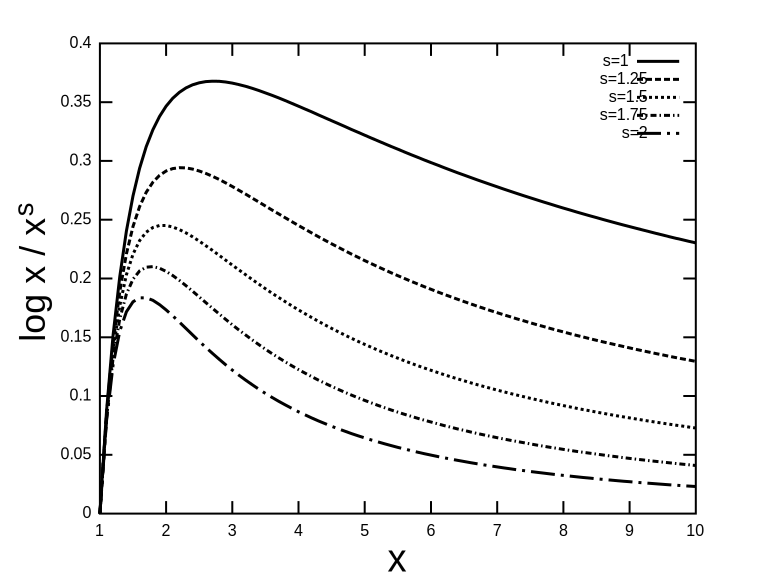
\includegraphics[width=0.75\textwidth]{images/logk_ks.pdf}
\caption{Behaviour of the function $f(x)=\frac{\ln x}{x^s}$ for different values of $s$.}
\label{fig:logk_ks}
\end{figure}

The summation in Equation \ref{eq:ent_zipfian_source}, for $x > 3$ is over a decreasing
function, regardless which $s$ we are considering. For that reason, we might approximate
using the Riemann sum approximation of an integral. This idea is illustrated in 
Figure \ref{fig:logk_k_integral}. As we have a decreasing function, the left Riemann sum
is a over estimate and the right Riemann sum is a under estimate.
\begin{equation}
\label{eq:riemmansumestimate}
\textmd{right Riemann sum} \leq \int_{a}^{b} f(x) dx \leq \textmd{left Riemann sum}
\end{equation} 
From Equation \ref{eq:riemmansumestimate} we might write
\begin{equation}
\label{eq:riemmansume1}
\sum_{n=4}^{N-1} \frac{\ln n}{n^s} \leq \int_{3}^{N-1} \frac{\ln x}{x^s} dx \leq \sum_{n=3}^{N-2} \frac{\ln n}{n^s}
\end{equation}
and
\begin{equation}
\label{eq:riemmansume2}
\sum_{n=4}^{N} \frac{\ln n}{n^s} \leq \int_{3}^{N} \frac{\ln x}{x^s} dx \leq \sum_{n=3}^{N-1} \frac{\ln n}{n^s}
\end{equation}
Using both Equations \ref{eq:riemmansume1} and \ref{eq:riemmansume2} we conclude that
\begin{equation}
\label{eq:riemmansume12}
\int_{3}^{N} \frac{\ln x}{x^s} dx \leq \sum_{n=3}^{N-1} \frac{\ln n}{n^s} \leq \int_{3}^{N-1} \frac{\ln x}{x^s} dx + \frac{\ln 3}{3^s}
\end{equation}
and by adding the two remaining terms to the summation, we get
\begin{equation}
\label{eq:riemmansume12f}
\int_{3}^{N} \frac{\ln x}{x^s} dx + \frac{\ln 2}{2^s} + \frac{\ln N}{N^s} \leq \sum_{n=1}^{N} \frac{\ln n}{n^s} \leq \int_{3}^{N-1} \frac{\ln x}{x^s} dx + \frac{\ln 3}{3^s} + \frac{\ln 2}{2^s} + \frac{\ln N}{N^s}
\end{equation}


\begin{figure}[htbp]
\centering
\includegraphics[width=0.75\textwidth]{images/logk_k_integral.pdf}
\caption{Riemann sum approximation of the integral.}
\label{fig:logk_k_integral}
\end{figure}

The integral in Equation \ref{eq:riemmansume12f} might be solved using an
integration by parts procedure. 
\begin{equation}
\label{eq:intparts}
\int \frac{\ln x}{x^s} dx = \int u dv = uv - \int v du
\end{equation}
We shall choose 
\begin{eqnarray}
\label{eq:intpartsuv}
u = \ln x           & \quad & dv = \frac{1}{x^s} dx \nonumber \\
du = \frac{1}{x} dx & \quad & v = \frac{x^{-s+1}}{1-s} 
\end{eqnarray}
Solving the integral, for $s \neq 1$, we have
\begin{eqnarray}
\label{eq:intpartsol}
\int \frac{\ln x}{x^s} dx &=& \frac{x^{1-s}}{1-s} \ln x - \int \frac{x^{1-s}}{1-s} \frac{1}{x} dx \nonumber \\
        &=& \frac{x^{1-s}}{1-s} \ln x - \frac{1}{1-s} \int x^{-s} dx \nonumber \\
        &=& \frac{x^{1-s}}{1-s} \ln x - \frac{x^{1-s}}{(1-s)^2} + c \nonumber \\
        &=& \frac{x^{1-s}}{1-s} \left( \ln x - \frac{1}{1-s} \right) - c \textmd{.}
\end{eqnarray}
When $s=1$ the integral will
result in
\begin{equation}
\label{eq:intpartss1}
\int \frac{\ln x}{x} dx = \frac{(\ln x)^2}{2} + c \textmd{ .}
\end{equation}

 
Using Equations \ref{eq:ent_zipfian_source}, \ref{eq:riemmansume12f} and \ref{eq:intpartsol}
we are able to calculate the bounds of the entropy of a Zipfian distributed source
for given $s$ and $N$. Figure \ref{fig:entropy_N_s} presents some results, where
the value of the entropy is given by the average of the upper and lower bounds given
by Equation \ref{eq:riemmansume12f} in conjunction with Equation \ref{eq:ent_zipfian_source}.
The lowe graph in Figure \ref{fig:entropy_N_s} presents the width of the interval to which
the estimated entropy is bouned. We might observe
that the entropy decreases with $s$, increases with $N$ and saturates as $s$ decreases towards zero.


\begin{figure}[htbp]
\centering
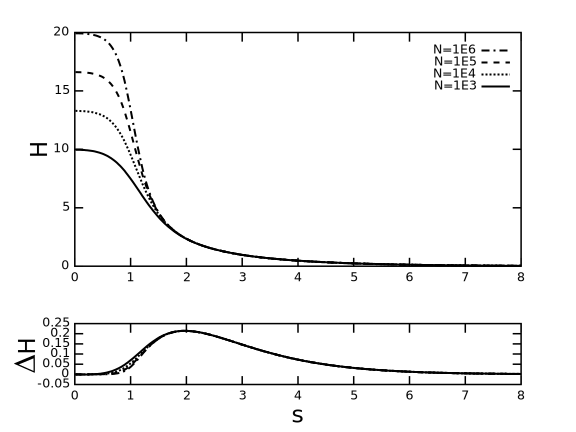
\includegraphics[width=0.75\textwidth]{images/entropy_N_s_limits_fulldh_pb.pdf}
\caption{Entropy $H$ (given in bits) as a function of the Zipf exponent $s$ and the number of types $N$. 
The upper plot presents the average Entropy given by the estimated presented and the lower plot gives
the difference between the lower and upper bounds in the estimation.}
\label{fig:entropy_N_s}
\end{figure}




\subsubsection{Entropy of Real Texts}
In this section we compare the results from the estimation proposed above with values
of entropy computed from real texts. In order to state such comparisons we are going 
to use a few text corpora: the top 100 most downloaded books in the Gutenberg database;
the complete work of William Shakespeare; and Ulysses by James Joice. 
We used GNU utilities to parse and transform these texts and then count the
frequency of occurrence of words in each corpus, creating a word-frequency
data-table. This data is afterwards used to compute the entropy of texts, which
are going to be compared to the estimated values in Table \ref{tab:entropytexts} bellow.

\begin{table}[h!]
\centering
\caption{Entropy of real texts (bits) compared with the estimated entropy (bits) using the parameter $N$ (number of types) found in the text and parameter $s$ (Zipf exponent) found by a Maximum Likelihood Estimation (MLE).}
\label{tab:entropytexts}
\begin{tabular}{| c | c | c | c | c |}
  \hline
  source & real entropy & $N$ & $s_{MLE}$ & estimated entropy \\
  \hline
  gutenberg     & 10.45 & 142515 & 1.14 & 9.17 \\
  shakespeare   & 10.02 & 27172  & 1.12 & 8.68 \\
  ulysses       & 10.63 & 29994  & 1.07 & 9.46 \\
  \hline
\end{tabular}
\end{table}

We might observe there is a significant deviation from the value estimated from the theoretical
procedures and the read value found in the corpora observed. Notice that the estimated value is consistently 
smaller. This deviation might be explained by a conjunction of discrepancies from our model and
the distribution of types found in each corpus. First, we know that in a real rank-frequency plot
there is a flattening in the low rank region. This flattening partially responsible for increasing
the entropy in the real data. This will we analyzed in the next section when we consider the 
generalized Zipf-Mandelbrot law \citep{mandelbrot1965}. Another aspect responsible for a higher 
entropy in our corpus is the staircase pattern in high rank region. The existence of many types
with the same frequency of occurrence proportionates a higher entropy in comparison with
a scenario where these types have distinct probability values. One third aspect that leads to
a higher entropy on our corpus is the fact that the probabilities estimated were based on
the maximum likelihood. As we pointed out before, it is necessary to perform a smoothing
in order to take in account these types which were not present in our sample. 
A Simple-Good Turing \citep{galesampson95} could be performed, what would  
shift the probability mass, decreasing the entropy value.



\subsection{Zipf-Mandelbrot's Entropy}
In order to take in account the flattening observed on low rank region of a Zipf plot, \cite{mandelbrot1965}
introduced a modification on the Zipf's law, adding a constant $q$ to the rank $k$, resulting in the Zipf-Mandelbrot's
law: $p_k(s,q,N) = C(k+q)^{-s}$, where the new normalizing constant (a generalization of a harmonic number)
is given by $C^{-1}=\sum_{n=1}^{N}(n+q)^{-s}$.

Applying the same steps to this generalized formulation, the entropy will be given by
\begin{equation}
\label{eq:ent_zipfmand_source}
\overline{H} = \frac{sC}{\ln 2} \sum_{k=1}^N \frac{\ln (k+q)}{(k+q)^s} - \frac{\ln C}{\ln 2} \textmd{ .}
\end{equation}
The new function $f(x)=(x+q)^{-s} \ln (x+q)$ will be decreasing for $x>e^{1/s}-q$. 
%The constant $q$ is a real value in the interval $[0;\infty)$, and $x \in \{1,2, \ldots, N\}$.
We shall then define an integer constant $K = \max(\lceil e^{1/s}-q \rceil,1)$ which guarantees that
the function $f(x)$ for $x>K \geq 1$.

Using the left and right Riemann sum again we find the inequalities bellow, which are
respectively equivalent to equations \ref{eq:riemmansume1} and \ref{eq:riemmansume2}:
\begin{equation}
\label{eq:riemmansummandel1}
\sum_{n=K+1}^{N-1} \frac{\ln (n+q)}{(n+q)^s} \leq \int_{K}^{N-1} \frac{\ln (x+q)}{(x+q)^s} dx \leq \sum_{n=K}^{N-2} \frac{\ln (n+q)}{(n+q)^s}
\end{equation}
\begin{equation}
\label{eq:riemmansummandel2}
\sum_{n=K+1}^{N} \frac{\ln (n+q)}{(n+q)^s} \leq \int_{K}^{N} \frac{\ln (x+q)}{(x+q)^s} dx \leq \sum_{n=K}^{N-1} \frac{\ln (n+q)}{(n+q)^s} \textmd{ .}
\end{equation}
From the above equations we conclude that
\begin{equation}
\label{eq:riemmansummandel12}
\int_{K}^{N} \frac{\ln (x+q)}{(x+q)^s} dx \leq \sum_{n=K}^{N-1} \frac{\ln (n+q)}{(n+q)^s} \leq \int_{K}^{N-1} \frac{\ln (x+q)}{(x+q)^s} dx + \frac{\ln (K+q)}{(K+q)^s}
\end{equation}
what is the equivalent to Equation \ref{eq:riemmansume12}. By adding the remaining terms we get the following boundaries
\begin{eqnarray}
\label{eq:riemmansumeboundsfinalmandelbrot}
B_l &=& \int_{K}^{N} \frac{\ln (x+q)}{(x+q)^s} dx + \sum_{n=1}^{K-1} \frac{\ln (n+q)}{(n+q)^s} + \frac{\ln (N+q)}{(N+q)^s} \nonumber \\ 
    &\leq& \sum_{n=1}^{N} \frac{\ln (n+q)}{(n+q)^s} \nonumber \\
    &\leq& \int_{K}^{N-1} \frac{\ln (x+q)}{(x+q)^s} dx + \sum_{n=1}^{K} \frac{\ln (n+q)}{(n+q)^s} + \frac{\ln (N+q)}{(N+q)^s} = B_u \textmd{ .}
\end{eqnarray}
The integral in Equation \ref{eq:riemmansumeboundsfinalmandelbrot} is solved by parts,
giving the same results as presented by equations \ref{eq:intparts} and \ref{eq:intpartss1},
considering that we have $x+q$ instead of $x$. By adding the parameter $q$, the distribution
suffers a flattening on the low rank values and consequently the entropy
of the source increases, what might be observed in Figure \ref{fig:entropy_H_q}, where
it is shown the effect of an increasing $q$ on distributions where $s$ and $N$ are kept constants.

%\begin{figure}[htbp]
%\centering
%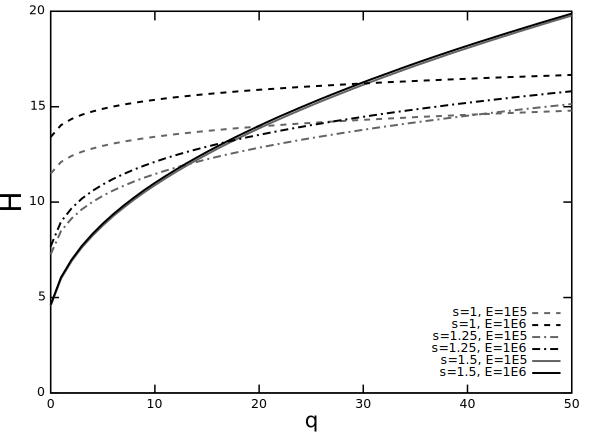
\includegraphics[width=0.8\textwidth]{images/zipfmandelbrotentropy_q.pdf}
%\caption{Effect of the parameter $q$ on the entropy $H$ (in bits) for a Zipf-Mandelbrot distribution.}
%\label{fig:entropy_H_q}
%\end{figure}

\begin{figure}
\centering
\begin{tabular}{cc}
  \subfloat[Effect of the parameter $q$ on the entropy $H$ (in bits) for a Zipf-Mandelbrot distribution.]{\label{fig:entropy_H_q}\includegraphics[width=0.45\textwidth]{images/zipfmandelbrotentropy_q.pdf}} &
  \subfloat[Compared effect of the parameter $s$ and $q$ when $N$ is fixed at $1E6$.]{\label{fig:zipfmandelbrot_entropy_sq_surface}\includegraphics[width=0.45\textwidth]{images/zipfmandelbrot_entropy_sq_surface.pdf}}
\end{tabular}
\caption{Those two plots illustrate the effect of the parameter $q$ on the entropy. A greater value of $q$ increases the entropy and the increase step is larger when the value of $s$ is bigger.}
\label{fig:entropy_q_s_effect}
\end{figure}




Table \ref{tab:entropytexts2} presents a new comparison between the entropy estimates and the
entropy found in real text data. We might observe that the usage of the Zipf-Mandelbrot model
improved the estimation of the entropy of real data. In order to achieve
a better approximation, we believe it is necessary to take in account 
the other aspects mentioned previously. 

\begin{table}[h!]
\centering
\caption{Entropy of real texts (bits) compared with the estimated entropy (bits) using the parameter $N$ (number of types) found in the text, parameter $s$ (Zipf exponent) found by a Maximum Likelihood Estimation (MLE) and the parameter $q$ found empirically.}
\label{tab:entropytexts2}
\begin{tabular}{| c | c | c | c | c | c |}
  \hline
  source & real entropy & $N$ & $s_{MLE}$ & q & estimated entropy \\
  \hline
  gutenberg     & 10.45 & 142515 & 1.14 & 3 & 11.07 \\
  shakespeare   & 10.02 & 27172  & 1.12 & 3 & 10.92 \\
  ulysses       & 10.63 & 29994  & 1.07 & 2 & 10.64 \\
  \hline
\end{tabular}
\end{table}


% python simplegoodturing_txt_entropy.py carroll-alice.txt
%        tokens      N (types)        entropy     gt entropy    sgt entropy   katz entropy
%  3.411000e+04   3.016000e+03   8.486082e+00   4.817249e+00   8.521606e+00   8.502261e+00
%
% python simplegoodturing_txt_entropy.py shakespeare-hamlet.txt
%        tokens      N (types)        entropy     gt entropy    sgt entropy   katz entropy
%  3.736000e+04   5.447000e+03   9.045087e+00   4.772809e+00   9.077038e+00   9.064729e+00
%
% python simplegoodturing_txt_entropy.py shakespeare-macbeth.txt
%        tokens      N (types)        entropy     gt entropy    sgt entropy   katz entropy
%  2.314000e+04   4.017000e+03   9.003743e+00   5.075033e+00   8.996533e+00   8.986618e+00
%
% python simplegoodturing_txt_entropy.py shakespeare-completeworks.txt
%        tokens      N (types)        entropy     gt entropy    sgt entropy   katz entropy
%  1.173902e+06   2.984700e+04   9.522252e+00   4.503280e+00   9.556085e+00   9.533598e+00
%
%python simplegoodturing_txt_entropy.py ulysses.txt
%        tokens      N (types)        entropy     gt entropy    sgt entropy   katz entropy
%  3.258310e+05   3.439100e+04   1.019018e+01   5.532290e+00   1.025373e+01   1.023023e+01

% file = carroll-alice.num, s = 1.120 	 s_sgt = 1.119
% file = shakespeare-completeworks.num, s = 1.149 	 s_sgt = 1.148
% file = shakespeare-hamlet.num, s = 1.090 	 s_sgt = 1.089
% file = shakespeare-macbeth.num, s = 1.073 	 s_sgt = 1.073
% file = ulysses.num, s = 1.097 	 s_sgt = 1.096


\begin{table}[h!]
\centering
\caption{This table presents the entropy of real texts (bits) with a Simple Good-Turing smoothing applied. They are compared to the estimated entropy (bits) using the parameter $N$ (number of types) found in the text, parameter $s$ (Zipf exponent) found by a Maximum Likelihood Estimation (MLE) and the parameter $q$ found by visual inspection.}
\label{tab:entropytexts2}
\begin{tabular}{| c | c | c | c | c | c | c |}
  \hline
  source & entropy & after sgt & $N$ & $s_{MLE}$ & q & estimated \\
  \hline
  carroll alice        & 8.49  & 8.79  & 3016  & 1.12 & 2.5 & 8.78  \\
  shakespeare hamlet   & 9.04  & 9.08  & 5447  & 1.09 & 1.5 & 9.07  \\
  shakespeare macbeth  & 9.00  & 8.76  & 4017  & 1.07 & 1   & 8.76  \\
  shakespeare complete & 9.52  & 9.56  & 29847 & 1.15 & 1.5 & 9.56  \\
  joyce ulysses        & 10.19 & 10.25 & 34391 & 1.10 & 1.5 & 10.24 \\
  \hline
\end{tabular}
\end{table}



In real texts, rare words appear in a staircase pattern in the end of the long tail of the distribution. 
It is said to be caused by the undersample these words suffer. In order to investigate the effect of this
staircase pattern on the entropy measure we make a substitution on the types with rank over $10E3$ by
the corresponding ideal Zipfian model. Figure \ref{fig:entropy_estimation_error_N_zipf_staircase_removal_ideal} 
the new probability-rank plot after the substitution. In Figure \ref{fig:entropy_estimation_error_N3}
we compare the value of the entropy for the data up to a specific range of rank and the entropy estimated 
by the method here proposed. We are taking in account the coherence in Zipf (see Section \ref{sec:coherencezipf})
and of that reason, a subset of the types up to a certain rank also constitute a set in which the same Zipf's law holds.


\begin{figure}
\centering
\begin{tabular}{cc}
  \subfloat[Frequency-rank plot where the types with rank over $10E3$ were substituted by an ideal Zipf model to remove the staircase pattern.]{\label{fig:entropy_estimation_error_N_zipf_staircase_removal_ideal}\includegraphics[width=0.45\textwidth]{images/entropy_estimation_error_N_zipf_staircase_removal_ideal.pdf}} &
  \subfloat[Difference between the real entropy and the estimated entropy as a function of $N$ (the number of types).]{\label{fig:entropy_estimation_error_N3}\includegraphics[width=0.45\textwidth]{images/entropy_estimation_error_N3.pdf}} 
\end{tabular}
\caption{The frequencies of Ulysses types are used to investigate the effect of the staircase pattern on difference between the real entropy and the estimated entropy proposed here.}
\label{fig:stpatt_entropy}
\end{figure}





\subsection{Emergence of Zipf's Law}
Zipf’s law for word frequencies could be the manifestation of a complex system 
operating between order and disorder. \cite{ramon2003,cancho2005} proposes a model to attest the
emergence of the Zipf's law in the balance in communication between information
transfer and the cost necessary to achieve communication. It take into compromise the principle of the least 
effort applied on the listener and speaker, creating a cost function.

Every language use symbolic references and signals to carry information.
We might, for example, consider words as our signals, and each one of them
make reference to one or more meaning or object in the real world.
The model proposed by \cite{ramon2003,cancho2005} assumes there are two finite sets:
the set of signals (words) $S = \{ s_1, s_2, \ldots , s_n \}$ and the set of 
stimuli (meanings) $R = \{ r_1, r_2, \ldots , r_n \}$. Signals are connected
to stimuli and that connections are defined by a binary $n \times m$ matrix
$A = \{ a_{ij} \}$ where $a_{ij} = 1$ if $s_i$ and $r_j$ are linked and
$a_{ij} = 0$ otherwise. The presented links in matrix $A$ don't claim that certain
words in $S$ refer to stimuli in $R$. When an element $a_{ij}$ is equals to one,
there is no imposed reference from the $i$-th word in the set $S$ and the
$j$-th stimuli in the set $R$, but it is stated that only an association between them exists.
Words create activation in different areas in the brain \citep{pulvermuller2003}. 
Nouns tend to activate
visual areas, verbs usually activate motor areas if the action can be performed by
the individual and visual areas otherwise. The activation of different areas is
a result of the associations created with different types of stimuli experienced with
the word. The word \textit{write}, for example, is associated with the motor stimuli
of the action of writing and the visual stimuli of the objects used in writing.
The definition of the meaning of a word is still an open problem, and the complexity
in the definition arises from the interaction between different stimuli.
It is reasonable to assume that a factor that influences a word frequency of usage
is the number of associations with different stimuli. The more stimuli a word is
associated to, the highest is its probability of occurrence. The fact that some 
words have no apparent meaning, such as prepositions, conjunctions and articles, 
does not imply that they don't have associations with stimuli. Words that apparently
don't carry meaning are the words with the highest frequencies, for example,
`the', `of', `of', `to' and `a'. These words are going to present the more connection
 with stimuli, which are merely associative and referential links.

The probability that a signal (word) $s_i$ is associated with a stimulus (meaning) $r_j$,
in a given communication system, is given by
\begin{equation}
p(s_i, r_j) = \frac{a_{ij}}{\Vert A \Vert}
\label{eq:prob_sr}
\end{equation}
where $\Vert A \Vert$ is the normalization factor 
\begin{equation}
\Vert A \Vert = \sum_i \sum_j a_{ij} \textmd{ .}
\end{equation}

The number of stimuli associated to a given signal $s_i$ is defined as
$\mu_i = \sum_{k=1}^m a_{ik}$. The probability of the signal $s_i$ is 
$p(s_i) = \sum_{j=1}^m p(s_i, r_j)$. Using this last definition and
substituting Equation \ref{eq:prob_sr} into it, we get
\begin{equation}
p(s_i) = \frac{\mu_i}{\Vert A \Vert} \textmd{ .}
\label{eq:prob_s}
\end{equation} 
Similarly, we define the number of signals associated to a certain stimulus
by $\omega_j = \sum_{k=1}^m a_{kj}$ and the probability of a given stimulus
is given by $p(r_j) = \sum_{k=1}^m p(s_k , r_j)$ and using the same substitution
with Equation \ref{eq:prob_sr} we get
\begin{equation}
p(r_j) = \frac{\omega_j}{\Vert A \Vert} \textmd{ .}
\label{eq:prob_r}
\end{equation}

What Equation \ref{eq:prob_s} states is that a word is used with a probability 
proportional to the number of stimuli it is associated to. This assumption is
supported by the fact that word frequency and number of meanings are positively
correlated \citep{manning1999}. This probability is dependent on the internal
organization of the communication system, on the other hand, the Equation
\ref{eq:prob_r} is related to the frequency of what we talk about, which is
dedicated to the outside world. The previous one seems really important
in the language communication model, but communication in human language
is ofter detached from the here and now \citep{hockett1960}.
``It is hard to establish from the state of the art of cognitive science
whether displaced speech acts are entirely controlled by the internal structure
of the communication system or not'' \citep{cancho2006}.

The signal entropy is given by
\begin{equation}
H(S) = - \sum_{i=1}^{n} p(s_i) \log p(s_i)
\end{equation}
and the mutual information between the signal and stimulus is expressed by
\begin{equation}
I(S,R) = \sum_{\substack{i=1\\ j=1}}^{n,m} p(s_i, r_j) \frac{\log p(s_i, r_j)}{p(s_i) p(r_j)} \textmd{ .}
\end{equation}
\cite{cancho2005} proposes to define a function $\Omega$ that a communication system must
minimize. ``The function is a combination of the goal of communication, that is, maximizing the 
information transfer between the set of signals and the set of stimuli, $I(S, R)$, and the constrains 
imposed by the biology of the communication system, which tend to minimize $H(S)$, the entropy associated 
to signals. $H(S)$ is the cost of the communication'' \citep{cancho2005}. The function $\Omega$ is
defined as a linear combination of the factors involved,
\begin{equation}
\Omega(\lambda) = - \lambda I(S,R) + (1-\lambda) H(S) \textmd{ ,}
\end{equation}
where the parameter $\lambda$ is such that $0 \leq \lambda \leq 1$ and controls the balance between 
the information transference and cost. When $\lambda < 1/2$, the cost of word use is prioritized over
the cost of information transfer. The extremes values $\lambda = 0$ and $\lambda = 1$ happen when just 
one factor is considered, word use and information transfer, respectively.

In order to minimize $\Omega(\lambda)$, \cite{cancho2005} uses a Monte Carlo algorithm.
The results for different values of $\lambda$ (compromise between word use and information transfer) 
are presented in the Figure \ref{fig:cancho_figA}. It shows an abrupt jump in the information transfer
which takes place at a critical value of $\lambda = \lambda^\ast = 1/2 - \epsilon$, where $\epsilon$
is a small positive value ($\epsilon \approx 0.002$ in Figure \ref{fig:cancho_figA}). The frequency versus rank
relation is presented in Figure \ref{fig:cancho_figB}. We observe that Zipf's law is found at the sharp increase in
$I(S,r)$ at $\lambda \approx 1/$.


\begin{figure}
\centering
\begin{tabular}{cc}
  \subfloat[$I(S, R)$, the information transfer between words and meanings, versus $\lambda$, the parameter regulating the balance between maximizing $I(S, R)$ and minimizing the entropy of words.]{\label{fig:cancho_figA}\includegraphics[width=0.45\textwidth]{images/cancho_figA.pdf}} &
  \subfloat[$P(i)$, the probability of the $i$-th most likely word in the system for $\lambda  = 0.49$ (circles), $\lambda = 0.498$ (squares) and $\lambda = 0.5$ (diamonds). The dashed line contains the theoretical curve for $\lambda = 0.498$.]{\label{fig:cancho_figB}\includegraphics[width=0.45\textwidth]{images/cancho_figB.pdf}}  
\end{tabular}
\caption{Some computational results on the model where meaning probabilities are governed by the internal structure of the communication system. The size of the system is $n = m = 400$ (i.e. 400 words and meanings). Figure reproduced from \cite{cancho2005}.}
\label{fig:cancho}
\end{figure}

From the results presented in Figure \ref{fig:cancho} and comparing with the frequency-rank relations
for phones, diphons, triphones, syllables and words presented Figure \ref{fig:ulysses_compared_nphones_probabilities}
and \ref{fig:ulysses_compared_words_probabilities}, we conclude that the smaller unities of speech 
behave as a system whose parameter $\lambda < \lambda^\ast$, a system in which the cost of use of symbols
is prioritized over the cost of information transfer. That result would be expected, since phones, diphones,
triphones and syllables don't carry any meaning, or are quite inefficient in matters concerning transmission of information. 
Among the examples presented here, only a system that use words as its symbols happen to have a balance between 
signal use and information transfer, and for that reason the Zipf's law is observed in frequency-rank relation
on words. We might conclude that words hold a very special position on the language structuring, being 
responsible to balance information transfer and use.






\section{Coherence in Zipf}
\label{sec:coherencezipf}
\cite{cristelli2012} proposes the idea that a Zipfian distribution is observed in group 
depending on the number of events and also ``requires a fundamental property of the sample
distribution which we call `coherence' and it corresponds to a `screening' between various
elements of the set'' \cite{cristelli2012}. They present the classical example of city sizes, 
where the data from each European country alone has a Zipf law in it, but the data from
all European country combined does not produce this power law pattern anymore. Another
interesting example present is the evolution of the Gross domestic product (GDP) of the 
countries of the world. The data from 1900 to 2008 shows a progressive approach to a
Zipf law, what is hypothesized to be caused by globalization, creating a coherence among
world's economies.

A question arises, whether a subset of the original Zipfan distributed set would also
present the same power law pattern. The answer to this question is not straightforward,
and is seems reasonable to assume that different types cause different contributions 
to the structure of the group. It is intuitive that, a subset of the original set, 
made of the group of most frequent types, will also present the same power law pattern,
since the ratio of two subsequent types will still be the same. Consider the Zipf's equation,
rewritten here for convenience,
\begin{equation} 
f(k; s, N) = \frac{1/k^s}{\sum_{n=1}^{N} 1/n^s} = C / k^s \textmd{ .}
\end{equation}
Discarding the $M$ least frequent types will only produce a change in the constant $C$,
and therefore the relation among the remaining types will be preserved.

Consider now the situation where the most frequent types are withdrawn. This will lead 
to a change in the relationship among the remaining items. Lets suppose the first $k^\ast$
most frequent items are removed. We rewrite the Zipf's equation using a new rank
variable $k' = k - k^\ast$. As we remove the most frequent items, the total number of
tokens in out dataset will be reduced to $N'$ and we want now to attest what is the 
new relation between rank and frequency of occurrence, if their product is roughly 
a constant, then we will find again a Zipf law. Since the dataset, regarding the
maintained items, has not changed, their frequencies of occurrence have also not changed.
The product between rank and frequency is given by
\begin{eqnarray}
k'^s f(k; s, N) &=& (k-k^\ast)^s f(k; s, N) \nonumber \\
                &=& k^s \left( 1 - \frac{k^\ast}{k} \right)^s f(k; s, N) \nonumber \\
                &=& \left( 1 - \frac{k^\ast}{k} \right)^s C \textmd{ .}
%                &=& (k^\ast)^s (-1)^s \sum_{n=0}^{\infty} {s \choose n} \left( \frac{k}{k^\ast} \right)^n (-1)^n
\end{eqnarray}
In order to investigate whether that value is a constant or not, we need
to evaluate $(1-k^\ast/k)^s$. As we are considering the case when $k > k^\ast$, 
we will have $0 < (1-k^\ast/k)^s < 1$.
If $k >> k^\ast$, we will have $(1-k^\ast/k)^s \approx 1$, and the relation between
rank and frequency will be approximately a constant. The smallest $k$ we are considering
is $k=k^\ast+1$, in which case, we shall have $(1-k^\ast/k)^s = (k^\ast+1)^{-s}$, 
what will lead to the strongest deviation from Zipf law. These remarks might
be observed in Figure \ref{fig:newrelarion_s1_1}, where we present the effect of
drawing the $k^\ast$ most frequent types for $k^\ast = 1,10 , 100, \ldots$. 
The value of $(1-k^\ast/k)^s$ as a function of $k$ is presented in Figure \ref{fig:zipf_distortion_factor}
for some values of $s$ and $k^\ast$.


% For values of $k$ that are slightly greater than $k^\ast$, 
% we might calculate it using the generalization of the binomial formula
% \begin{equation}
% (1+X)^\alpha = \sum_{k=0}^\infty {\alpha \choose k} X^k
% \end{equation}
% and the generalized binomial coefficient is given by
% \begin{equation}
% \binom \alpha k = \frac{\alpha^{\underline k}}{k!} = \frac{\alpha(\alpha-1)(\alpha-2)\cdots(\alpha-k+1)}{k(k-1)(k-2)\cdots 1}
%   \quad\textmd{for } k\in \mathbb{N} \textmd{ and arbitrary } \alpha.
% \end{equation}


The new relation between rank and frequency, as we remove the $k^\ast$ most frequent
types is displayed in Figure \ref{fig:newrelarion_s1_1} for different values of
$k\ast$. The Zipf law doesn't hold anymore as the most frequent types are removed.
In fact, it is enough to remove the most frequent type, to make the Zipf law not 
valid anymore. This is know as the New York's effect, ``we cannot draw two or more 
`New York’s', for we would destroy the coherence of the set if we did'' \citep{cristelli2012}.


\begin{figure}[htbp]
\centering
\includegraphics[width=0.75\textwidth]{images/newrelarion_s1_1.pdf}
\caption{New relation between rank and frequency as the $k^\ast$ most frequent types are removed. Results obtained using an exponent $s=1.1$.}
\label{fig:newrelarion_s1_1}
\end{figure}

\begin{figure}[htbp]
\centering
\includegraphics[width=0.75\textwidth]{images/zipf_distortion_factor.pdf}
\caption{Distortion factor as a result of withdrawing the $k^\ast$ most frequent types.}
\label{fig:zipf_distortion_factor}
\end{figure}


Another possibility is to remove types from within the Zipf plot, and we want to investigate 
what will be the results on the new created data, whether it will hold a power law relation or not.
As previously argued, the highest frequency types, will suffer no distortion on the relation they
have among them, holding the same Zipf law. The types less frequent then the removed data will suffer
a distortion. Consider the removal of some middle frequency types, as explained in figure
\ref{fig:remove_kast_kastast}. The types with rank between $k^\ast$ and $k^{\ast\ast}$ will be removed
and the data originally ranked above $k^{\ast\ast}$ will have a new frequency-rank relation, as might
be expressed by 
\begin{eqnarray}
k'^s f(k; s, N) &=& (k-k^{\ast\ast}+k^\ast)^s f(k; s, N) \nonumber \\
                &=& (k-\Delta k^\ast)^s f(k; s, N) \nonumber \\
                &=& \left(1 - \frac{\Delta k^\ast}{k} \right)^s k^s f(k; s, N) \nonumber \\
                &=& \left(1 - \frac{\Delta k^\ast}{k} \right)^s C
\end{eqnarray}
From this relation we might observe that types with $k >> \Delta k^\ast$ will suffer a small distortion 
on the relation between frequency and rank. The distortion will be the same as the previously considered
in Figure \ref{fig:zipf_distortion_factor}, but changing $k^\ast$ by $\Delta k^\ast$ in the distortion factor 
equation. 


\begin{figure}[htbp]
\centering
\includegraphics[width=0.75\textwidth]{images/remove_kast_kastast.pdf}
\caption{Removal procedure of middle frequency types: the types ranked between $k^\ast$ and $k^{\ast\ast}$ (gray area) are removed.}
\label{fig:remove_kast_kastast}
\end{figure}



\cite{cristelli2012} suggest that the aggregation of different data, that present alone a Zipf law, will not present
the same frequency-rank behaviour, since these data come from different distributions and might not have coherence among
them. In order to verify this supposition we have generated random texts using different symbol probabilities. 
Each one of them present a Zipf like behaviour, in accordance with \cite{miller1957} and \cite{li1992}. 
The random texts created have 6 symbols and one word-break symbol. Symbols were randomly drawn, according
to a different set of probabilities for each text, until the text length reached $8 \times 10^4$ symbols.
Figure \ref{fig:freq_rank_random_data_cat_pb} present the Zipf relation observed in each random generated data
and also in the large data created by the concatenation of the previous seven, which also presents a Zipf law.
This could contradict what was expected by \cite{cristelli2012} or could corroborate that random text
don't present a truly Zipfian distribution pattern, the exponential decreasing frequency is just again
a mere byproduct of selecting rank as the independent variable.

\begin{figure}[htbp]
\centering
\includegraphics[width=0.75\textwidth]{images/freq_rank_random_data_cat_pb.pdf}
\caption{Frequency-rank relation of seven random generated texts, with different symbols probabilities, and the frequency-rank relation in the concatenation of those seven random texts.}
\label{fig:freq_rank_random_data_cat_pb}
\end{figure}




\section{Generalized Zipf}
The frequency rank relation suffer observable deviations from the power-law on the high- and low-rank regions.
The former one is usually explained as an effect of under-sampling of rare words in the corpus,
what create the stair case pattern. The last one is observed as a flattering in the upper part 
of the Zipf curve. To account for that behavior on the low-rank region, \cite{mandelbrot1965}
proposed a modified formula, given a generalized relation between rank and frequency of occurrence
\begin{equation}
\label{eq:zipfmandelbrot}
f(k;s,N,q) = C (k+q)^{-s} \textmd{ , }
\end{equation}
where the new parameter $q$ also characterize the distribution at hand and
the constant $C$ is now given by
\begin{equation}
C = \frac{1}{\sum_{n=1}^{N} (n+q)^{-s}} \textmd{ .}
\end{equation}
Note that this generalization becomes the previous Zipf's Law when $q=0$.
Asymptotically, the relation \ref{eq:zipfmandelbrot}, also known as
Zipf-Mandelbrot Formula, is equivalent to the power law \ref{eq:zipf_relation}, when $k >> q$.
The constant $C$ is the inverse of the generalized harmonic number, which has a limit
as $N$ tends to infinity only if $s>1$. It might also be called as the Riemann zeta function,
when $N\rightarrow\infty$: $\zeta(s) = \sum_{n=1}^\infty n^{-s}$. When $s=1$ we have the harmonic
series: $\zeta(1) = 1 + \frac{1}{2} + \frac{1}{3} + \cdots = \infty$; when $s=2$ the 
we get $\zeta(2) = 1 + \frac{1}{2^2} + \frac{1}{3^2} + \cdots = \frac{\pi^2}{6}$, 
which demonstration is known as the \textit{Basel problem}, first posed by Pietro Mengoli in 1644 
and solved by Leonhard Euler in 1735.
As our constant $C$ tends to the inverse of the Riemann zeta function in the limit, it might be
also seen as Dirichlet series over the M\"obius function $\mu (n)$, that means
\begin{equation}
\lim_{N \rightarrow \infty} C = \frac{1}{\zeta(s)} = \sum_{n=1}^{\infty} \frac{\mu(n)}{n^s} \textmd{ .}
\end{equation}

\cite{miller1957,mandelbrot1965} propose the model of \textit{intermittent silence} to
study the statistical properties of languages. Mandelbrot proposes 
that the cost of producing a word is proportional to its length in characters,
and defined the information content of a word as the Shannon entropy.
Minimizing the average cost per unit of information, he showed that the
random placement of spaces leads to Zipf's rule, which is actually the optimal
solution, which might be achieved as a result of language evolution.
The use of \textit{space} as a word-delimiter 
would cause an exponential increase in the number of words regarding
its length, and that would hold even if the characters used don't
are not equiprobable \citep{li1992}. That behavior, on the contrary, is not
observed, and the relation relation between the number of existing words
and their length is not even monotonically increasing, as we observed 
in the results presented in Figure \ref{fig:wordsNumVsLength}.

The generalization proposed in \ref{eq:zipfmandelbrot}, is more suited to
follow the empirical observations. According to \cite{mandelbrot1965},
the flatness presented in the low-rank regions depends on the `wealth 
of vocabulary' of the subject, and the parameters $C$, $q$ and $s$
are dependent on the subject, and they ``do not characterize a language,
although it may well be that different languages favor different ranges
of values for the parameters''.

\cite{manin2009} present a minimization procedure of the cost ratio
$C^\ast = C/H$, where $C$ is the average cost of producing words 
and $H$ is the entropy per word. \cite{manin2009} shows that there is one
Ansatz that leads to the Zipf's law or the Zipf-Mandelbrot's law. 
If we consider that each word $w_k$ happens with probability $p_k$,
we assign an unspecified value $C_k$ to the cost of producing the word $w_k$.
The word's information content is given by $H_k = - \log_2 p_k$. 
The average cost per word is then calculated by
\begin{equation}
C = \sum_k p_k C_k
\end{equation}
and the average entropy per word by
\begin{equation}
H = - \sum_k p_k \log_2 p_k \textmd{ .}
\end{equation}

The probabilities of the words are such that $\sum_k p_k = 1$ must hold.
We wish to minimize the cost ratio $C^\ast = C/H$, so the Lagrange 
multipliers are used, defining the Lagrange function 
\begin{equation}
\Lambda(p_k, \lambda) = C/H + \lambda \cdot \Big(\sum_k p_k - 1 \Big) \textmd{ .}
\end{equation}
Finding the minimum of the cost ration is equivalent to find the 
stationary point for the Lagrange function, which correspond
to those points where the partial derivatives of $\Lambda$ are zero, i.e. 
$\nabla \Lambda = 0$. That means we seek for
\begin{equation}
\frac{\partial}{\partial p_k} \left( C^\ast + \lambda \sum_j p_j \right) = 0 \textmd{ .}
\end{equation}
Performing the differentiation, we obtain
\begin{equation}
\frac{C_k}{H} + \frac{C}{H^2} \left( \log_2 p_k + \frac{1}{\ln 2}\right) + \lambda = 0 \quad , \forall k \textmd{ .}
\end{equation}
The frequency $p_k$ is given by
\begin{equation}
p_k = 2^{-\lambda H^2/C} 2^{- 1/ \ln_2} 2^{-C_k H /C} \textmd{ .}
\end{equation}
A power law for frequencies could only result from the Ansatz
\begin{equation}
\label{eq:ansatz}
C_k = C_0 \log_2 k \textmd{ ,}
\end{equation}
what leads to 
\begin{equation}
p_k = 2^{-\lambda H^2/C} 2^{- 1/ \ln_2} k^{-C_0 H/C} \textmd{ ,}
\end{equation}
that might be rewritten in the Zipf form by $p_k = C' k^{-s}$, where the constant are defined by 
$C' = 2^{-\lambda H^2/C} 2^{- 1/ \ln_2}$ and $s = C_0 H/C$.

According to \cite{manin2009}, the relation \ref{eq:ansatz} ``is a much more plausible argument
(...) which does not depend on any assumptions about word length at all.
Suppose words are stored in some kind of an
addressable memory. For simplicity, one can imagine a linear array of
memory cells, each containing one word. Then, the cost of retrieving the
word in the $k$th cell can be assumed to be proportional to the length of its
address, that is to the minimum number of bits (or neuron firings, say)
needed to specify the address. And this is precisely $\log_2 k$''\citep{manin2009}.

Using a different Ansatz
\begin{equation}
\label{eq:ansatz2}
C_k = C_0 \log_2 ( k + q) \textmd{ ,}
\end{equation}
that would lead to the Zipf-Mandelbrot's law.
This law is ``obtained from a model optimizing the information/cost ratio
with no assumptions about word lengths. This model is not equivalent to the random typing model, and
allows the optimum to be achieved via local dynamics, i.e. in a causal,
rather than teleological manner. However, the two parameters of the
resulting distribution, $s$ and $q$, are not independent, and as a result, it
does not provide a reasonable fit to the empirical data''\citep{manin2009}.


%Moreover, a
%theorem of Shannon (1948) (Section 7, Theorem 3) suggests that even the
%condition of independence between characters can be relaxed and
%replaced with ergodicity of the source.
%
%language is optimal in the sense that it minimizes the average ratio of
%production cost to information content.





\section{Heaps' Law}
Zipf's law is perhaps the best evidence of an universal physical law, which
has drawn a considerable attention on the academia. Many different explanations
of Zipf's law has been given: as a result of a random process \citep{miller1957,li1992},
or due to the principle of least effort \citep{zipf1949, ramon2003}, or 
a Boltzmann-type approach \citep{during2008}, or avalanche dynamics in a
critical system \citep{bak1999}.

Power laws are referred to have a scale invariance behaviour, making it impossible
to define a characteristic scale. Language statistics present more that one
dimension, we might consider the frequency of occurrence as a independent variable,
or the text (or utterance) length $T$ (the number of tokens in a sample), 
or even the vocabulary size $V_T$ (the number of types present in a sample).
The relation between text length $T$ and vocabulary size $V_T$ is known as
Heap's law (also called Herdan's law), which states that the vocabulary
$V_L$ grows in a sublinear form with the text length $T$,
\begin{equation}
\label{eq:heaps}
V_T \propto T^\alpha \textmd{ , \ \ } \alpha < 1 \textmd{ .}
\end{equation}

\cite{vanLeijenhorst} shows that Heaps' law and the generalized Zipf's law are related.
Assuming a Mandelbrot distribution, it is possible to mathematically derive Heaps' law.
If both Zipf's law and Heaps' law hold, than their exponents are related by $\alpha = 1/s$.
It means that the Zipf's exponential coefficient must be greater then one, in order
to make $\alpha < 1$, a plausible value. As we observed previously, the Zipf exponent 
for natural phenomena always presented an exponent greater than one, what differed from 
the random generated texts. In fact, \cite{linyua2010} shows that the relation
$\alpha = 1/s$ is only an asymptotic solution that every large-size system holds
when $s > 1$. 

A formal derivation of Heaps' law is given by \cite{vanLeijenhorst} and we present it here.
For that purpose we are going to call $\mathcal{W}$ the set of words in a text
(the set of tokens in a sample) and $\mathcal{D}$ is the set of different words in
a text (the set of types in a sample). For simplicity reason, we shall consider that
the occurrence of each word is independent one from another. We are characterizing 
a text as a random process of independently drawing words from a set with replacement.
After $n$ words were drawn, we will end up with a set $\mathcal{W}_n$ with length $n$
and a set $\mathcal{D}_n$ with length $m_n \leq n$. The Heaps' law states a relation
between $m_n$ and $n$, and we are particularly interested in the behaviour as $n \rightarrow \infty$.
In that case, we shall deal with $\mathcal{D}$ as the underlying lexicon of a language,
the set of all possible types. In order to know what is the expected number of different
words in sequence of independently tokens drawn from a set, we shall analyze the
$n$-th draw in detail. 

As the $n$-th token is drawn, there might be two possibilities: 1) the $n$-th token
is a new type, and therefore is not present in $\mathcal{D}_{n-1}$; or 2) the $n$-th token
is already in $\mathcal{D}_{n-1}$, and therefore the length of $\mathcal{D}_{n}$ 
is equal to the length of $\mathcal{D}_{n-1}$. After $n$ draws were made, we shall consider
$w_n$ as the $n$-th token in the sequence, and we want to
find what is the probability that there are $a$ different types, $\Pr (m_n = a)$.
There may not be more types then tokens, so $\Pr (m_n = a) = 0$ if $a>n$. 
If $a \leq n$ we shall have
\begin{eqnarray}
\Pr(m_n = a) &=& \Pr(m_{n-1} = a-1 \wedge w_n \notin \mathcal{D}_{n-1}) + 
                 \Pr(m_{n-1} = a \wedge w_n \in \mathcal{D}_{n-1}) \nonumber \\
             &=& \Pr(m_{n-1} = a-1) \Pr(w_n \notin \mathcal{D}_{n-1}) + \nonumber \\
             &&  \Pr(m_{n-1} = a) \Pr(w_n \in \mathcal{D}_{n-1})
\end{eqnarray}
We know that $\Pr(w_n \notin \mathcal{D}_{n-1}) = 1 - \Pr(w_n \in \mathcal{D}_{n-1})$, and the 
former one might be given by the sum of the probabilities of every word in the underlying lexicon
not belonging to the set $\mathcal{D}_{n-1}$
\begin{eqnarray}
\Pr(w_n \notin \mathcal{D}_{n-1}) &=& \sum_{i\in\mathcal{D}} \Pr(w_n = i \wedge i \notin \mathcal{D}_{n-1}) \nonumber \\
                                 &=& \sum_{i\in\mathcal{D}} \Pr(w_n = i) \Pr(i \notin \mathcal{D}_{n-1}) \nonumber \\
                                 &=& \sum_{i\in\mathcal{D}} p_i (1-p_i)^{n-1}
\end{eqnarray}
where $p_i$ stands for the underlying probability of the $i$-th word in the lexicon, and
$\Pr(i \notin \mathcal{D}_{n-1})$ is the probability that the $i$-th word has not happened
after $n-1$ draws, so it must be equals to $(1-p_i)^{n-1}$.

For convenience, We are going to use the same notation as \cite{vanLeijenhorst}
\begin{equation}
S_n = \sum_{i\in\mathcal{D}} p_i (1-p_i)^{n-1}
\end{equation}
\begin{equation}
M_n = \sum_{i\in\mathcal{D}} (1-p_i)^{n}
\end{equation}
from which we might find the relation bellow
\begin{eqnarray}
M_{n-1} - M_n &=& \sum_{i\in\mathcal{D}} (1-p_i)^{n-1} - \sum_{i\in\mathcal{D}} (1-p_i)^{n} \nonumber \\
              &=& \sum_{i\in\mathcal{D}} (1-p_i)^{n-1} \left( 1 - (1 - p_i) \right) \nonumber \\
              &=& \sum_{i\in\mathcal{D}} p_i (1-p_i)^{n-1} = S_n \textmd{ .}
\end{eqnarray}
Using $N(n,a) = \Pr(m_n = a)$ we have $N(1,1)$, since only one token was drawn. As previously
stated, $N(n,a) = 0$ if $n < a$ and for $n \geq a$ shall have
\begin{equation}
N(n,a) = N(n-1,a-1) S_n + N(n-1,a)(1-S_n)
\end{equation}
what suggests a recurrence relation to find the value of $N(n,a)$.

After $n$ tokens were drawn, the expected number of types is given by
\begin{align}
\label{eq:expectedmn}
E[m_n] &= \sum_{a=1}^n a N(n,a) \nonumber \\
       &= \sum_{a=1}^n a \left( N(n-1,a-1) S_n + N(n-1,a)(1-S_n) \right) \nonumber \\
       &= S_n \sum_{a=1}^n a N(n-1,a-1) + (1-S_n) \sum_{a=1}^n a N(n-1,a) \nonumber \\
       &= S_n \sum_{a=1}^n a N(n-1,a-1) + (1-S_n) \left[ n N(n-1,n) + \sum_{a=1}^{n-1} a N(n-1,a) \right]\nonumber \\
       &= S_n \sum_{a=1}^n a N(n-1,a-1) + (1-S_n) \left[ 0 + E[m_{n-1}] \right]\nonumber \displaybreak[3]\\
       &= S_n \left[ \sum_{a=1}^n (a-1) N(n-1,a-1) + \sum_{a=1}^n N(n-1,a-1) \right] + (1-S_n) E[m_{n-1}] \nonumber \\
       &= S_n E[m_{n-1}] + S_n \sum_{a=1}^n N(n-1,a-1) + (1-S_n) E[m_{n-1}] \nonumber \displaybreak[3] \\
       &= S_n \sum_{a=1}^n N(n-1,a-1) + E[m_{n-1}] \nonumber \displaybreak[3] \\
       &= S_n + E[m_{n-1}]
\end{align}


\cite{vanLeijenhorst} presents a formal proof that when the data is Zipfianly distributed,
it will lead to a Heaps behaviour on the increase number of types as the number of tokens
increase. We might wonder weather this sort of behaviour is characteristic only of Zipfian
distributed data, or whether it could happen with other type of distributions, or even with
every type of distribution. We present in the Figure \ref{fig:heapslaw_rdist} 
a computer simulation of the
expected number of types as the number of tokens increases, using three different discrete
probability distributions: binomial, uniform and zipf. For every one of them we considered
a sample of length $10^6$ and a lexicon of size $10^4$.

\begin{figure}[htbp]
\centering
\includegraphics[width=0.8\textwidth]{images/heapslaw_rdist.pdf}
\caption{The recurrence equation is used to estimate the expected number of types for a sample with a certain number of tokens. Different probabilities for set were used: binomial, uniform and zipf. All of them present a Heaps like behaviour.}
\label{fig:heapslaw_rdist}
\end{figure}

This behaviour is expected, since the sequence of $S_n$ used to compute $E[m_n]$ is such that
\begin{equation}
1 > S_1 > S_2 > \cdots > S_{n-1} > S_n > 0\textmd{ .}
\end{equation}
What might be verified by taking $S_n$ and writting it as a function of $S_{n-1}$.
\begin{align}
\label{eq:SnR}
S_n &= \sum_{i=1}^N p_i (1-p_i)^n \nonumber \\
    &= \sum_{i=1}^N p_i (1-p_i)^{n-1} (1 - p_i) \nonumber \\
    &= \sum_{i=1}^N p_i (1-p_i)^{n-1} - \sum_{i=1}^N p_i^2 (1-p_i)^{n-1} \nonumber \\
    &= S_{n-1} - \sum_{i=1}^N p_i^2 (1-p_i)^{n-1} = S_{n-1} - R
\end{align}
The latest term $R$ is a sum of positive values, and therefore is positive itself.
We may conclude then that $S_n > S_{n-1}$, and the sequence of $S_n$'s is a monotonically
decreasing sequence with increasing $n$.

Using Equation \ref{eq:expectedmn} and the fact that $E[m_0]=1$ and $S_0=1$ we might write
$E[m_n]$ in the following way:
\begin{equation}
\label{eq:sumexpctmn}
E[m_n] = \sum_{i=0}^n S_i \textmd{ .}
\end{equation}
The values of $S_i$'s are finite and therefore, for a finite sample, the number of types
observed is also finite. Considering the assyntotic behaviour, as $n \rightarrow \infty$,
we want to find the underlying number of types (lexemes) in a language vocabulary (lexicon).
To verify if the sum in Equation \ref{eq:sumexpctmn} converges, me might use the D'Alembert's criterion,
which states that
\begin{equation}
\label{eq:dalambert}
\lim_{n \to \infty} \left| \frac{S_n}{S_{n-1}} \right| = r
\end{equation}
and the sum will converge if $r <1$, it will diverge if $r > 1$ and it will be unconclusive
if $r=1$. 

We might then use the relation expressed in Equation \ref{eq:SnR} and express Equation
\ref{eq:dalambert} as
\begin{align}
\lim_{n \to \infty} \left| \frac{S_n}{S_{n-1}} \right| &= \lim_{n \to \infty} \left| \frac{S_{n-1} - R}{S_{n-1}} \right| \nonumber \\
       &= \lim_{n \to \infty} \left| 1 - \frac{R}{S_{n-1}} \right| = r
\end{align}
As $S_{n-1} > R > 0$, we may conclude that the sum will converge. 

We conclude then, that 
the behaviour of the expected number of types in a sample is a monotonically increasing
function of the sample size, converging to the underlying number of types in the vocabulary 
in question. Although the lexicon size may increase as the text length 
increases infinitely, the lexicon size has a limiting value.
% (what is a typical behaviour in random generated texts),
The expected value of the lexicon size is still finite and may be estimated given 
the distribution is known.
The lexicon growth behaviour in natural language is verified for some texts from the Guternberg 
Database. Figure \ref{fig:heapslawtexts} bellows present the relation between the text length and
the vocabulary size for 35 different books, all plotted in gray. The continuous black curve
presents the relation for the metabook created by the concatenation of all 35 books. As a reference,
it is also presented, by a dashed line, the 1:1 relation.
 

\begin{figure}[htbp]
\centering
\includegraphics[width=0.8\textwidth]{images/heapslawtexts.png}
\caption{The relation between the number of tokens and types in 35 books from Gutenberg Database is presented in gray. The dark curve is the result when all 35 books are concatenated and the dashed line is presented only as a reference, when the number of types is equals the number of tokens.}
\label{fig:heapslawtexts}
\end{figure}





